% VerA.web (public) Installationsanleitung
%
% Copyright © 2015, 2016, 2017, 2018
%	Thorsten Glaser <t.glaser@tarent.de>
% Copyright © 2014, 2015
%	Thorsten Glaser <thorsten.glaser@teckids.org>
% Copyright © 2013, 2014
%	Dominik George <dominik.george@teckids.org>
%
% Contains excerpts of configuration files licenced to the ASF under
% one or more contributor license agreements and published under the
% Apache License, Version 2.0 — see the global VerA.web LICENCE file
% for details, terms and the “NOTICE” file contents.
%
% Provided that these terms and disclaimer and all copyright notices
% are retained or reproduced in an accompanying document, permission
% is granted to deal in this work without restriction, including un‐
% limited rights to use, publicly perform, distribute, sell, modify,
% merge, give away, or sublicence.
%
% This work is provided “AS IS” and WITHOUT WARRANTY of any kind, to
% the utmost extent permitted by applicable law, neither express nor
% implied; without malicious intent or gross negligence. In no event
% may a licensor, author or contributor be held liable for indirect,
% direct, other damage, loss, or other issues arising in any way out
% of dealing in the work, even if advised of the possibility of such
% damage or existence of a defect, except proven that it results out
% of said person’s immediate fault when using the work as intended.
%-
% Characters requiring escaping:
% • { } # & _ % $ ⇒ quote by prepending a backslash \
% • \ → \textbackslash
% • ~ → \textasciitilde
% • ^ → \textasciicircum
% • (nbsp) → ~
% • (em dash) → \dash
%-
% TODO:
% - Unterkapitel "Securing OSIAM", mit den Berlinern zusammen, nach der Schnellinstallation

\documentclass{tarentanleitung}
\usepackage{tikz}
\usetikzlibrary{arrows,backgrounds,fit,positioning,shapes,shadows}

% VerA.web Fassung der Installationsanleitung
\newcommand{\vwiaversfassungnr}{5.0}
\newcommand{\vwiaversfassungmonat}{Februar}
\newcommand{\vwiaversfassungjahr}{2018}

% VerA.web Version
\newcommand{\vwiaverssw}{1.8.58}

% OSIAM-Version
\newcommand{\vwiaversosiam}{2.5}

% später entfernen
\newif\ifoa
\oatrue

\begin{document}
\tarentanleitung{Installationsanleitung VerA.web}{\vwiaverssw}
 {\vwiaversfassungnr}{\vwiaversfassungmonat}{\vwiaversfassungjahr}{veraweblogo}

% uncomment if this is a WIP that should not be published
\fancyfoot[RO,LE]{\leavevmode\usekomafont{pageheadfoot}⚠ Work in Progress, do not use}

% LaTeX Table of Contents for tarent
%
% Copyright © 2015
%	Thorsten Glaser <t.glaser@tarent.de>
%
% Provided that these terms and disclaimer and all copyright notices
% are retained or reproduced in an accompanying document, permission
% is granted to deal in this work without restriction, including un‐
% limited rights to use, publicly perform, distribute, sell, modify,
% merge, give away, or sublicence.
%
% This work is provided “AS IS” and WITHOUT WARRANTY of any kind, to
% the utmost extent permitted by applicable law, neither express nor
% implied; without malicious intent or gross negligence. In no event
% may a licensor, author or contributor be held liable for indirect,
% direct, other damage, loss, or other issues arising in any way out
% of dealing in the work, even if advised of the possibility of such
% damage or existence of a defect, except proven that it results out
% of said person’s immediate fault when using the work as intended.
%-
% include with 「% LaTeX Table of Contents for tarent
%
% Copyright © 2015
%	Thorsten Glaser <t.glaser@tarent.de>
%
% Provided that these terms and disclaimer and all copyright notices
% are retained or reproduced in an accompanying document, permission
% is granted to deal in this work without restriction, including un‐
% limited rights to use, publicly perform, distribute, sell, modify,
% merge, give away, or sublicence.
%
% This work is provided “AS IS” and WITHOUT WARRANTY of any kind, to
% the utmost extent permitted by applicable law, neither express nor
% implied; without malicious intent or gross negligence. In no event
% may a licensor, author or contributor be held liable for indirect,
% direct, other damage, loss, or other issues arising in any way out
% of dealing in the work, even if advised of the possibility of such
% damage or existence of a defect, except proven that it results out
% of said person’s immediate fault when using the work as intended.
%-
% include with 「% LaTeX Table of Contents for tarent
%
% Copyright © 2015
%	Thorsten Glaser <t.glaser@tarent.de>
%
% Provided that these terms and disclaimer and all copyright notices
% are retained or reproduced in an accompanying document, permission
% is granted to deal in this work without restriction, including un‐
% limited rights to use, publicly perform, distribute, sell, modify,
% merge, give away, or sublicence.
%
% This work is provided “AS IS” and WITHOUT WARRANTY of any kind, to
% the utmost extent permitted by applicable law, neither express nor
% implied; without malicious intent or gross negligence. In no event
% may a licensor, author or contributor be held liable for indirect,
% direct, other damage, loss, or other issues arising in any way out
% of dealing in the work, even if advised of the possibility of such
% damage or existence of a defect, except proven that it results out
% of said person’s immediate fault when using the work as intended.
%-
% include with 「\input{toc.tex}」 after \tarentanleitung{…}…

\addtocontents{toc}{\protect\thispagestyle{fancy}}
\addtolength{\cftsubsecnumwidth}{0.5em}
\addtolength{\cftsubsubsecindent}{0.5em}
\renewcommand{\cftsecleader}{\cftdotfill{\cftdotsep}}
\hypersetup{linkcolor = black}
\tableofcontents
\hypersetup{linkcolor = blue}
\newpage
」 after \tarentanleitung{…}…

\addtocontents{toc}{\protect\thispagestyle{fancy}}
\addtolength{\cftsubsecnumwidth}{0.5em}
\addtolength{\cftsubsubsecindent}{0.5em}
\renewcommand{\cftsecleader}{\cftdotfill{\cftdotsep}}
\hypersetup{linkcolor = black}
\tableofcontents
\hypersetup{linkcolor = blue}
\newpage
」 after \tarentanleitung{…}…

\addtocontents{toc}{\protect\thispagestyle{fancy}}
\addtolength{\cftsubsecnumwidth}{0.5em}
\addtolength{\cftsubsubsecindent}{0.5em}
\renewcommand{\cftsecleader}{\cftdotfill{\cftdotsep}}
\hypersetup{linkcolor = black}
\tableofcontents
\hypersetup{linkcolor = blue}
\newpage


\section{Einleitung}\label{sec:intro}

„VerA.web“ steht für Veranstaltungs‑ und Adreßverwaltung im „web“ (Internet).
VerA.web ist eine Open Source-Webanwendung, die die IT-gestützte Planung und
Durchführung von Anlässen, Konferenzen und anderen Veranstaltungen maßgeblich
unterstützt.

Die „Online-Anmeldung“ ermöglicht es Gästen, sich selbst zu Veranstaltungen
anzumelden, die für diese Prozedur freigeschaltet sind, sowie zu einer
Veranstaltung angemeldeten Delegationen, ihre Mitglieder selbst zu melden.
Die Installation und Nutzung der Online-Anmeldung ist optional.

\subsection{Über diese Anleitung}\label{subsec:aboutmanual}

Dieses Dokument beschreibt, wie das Veranstaltungsmanagement
VerA.web, optional mit Online-Anmeldung und (falls nötig) dem
von der Online-Anmeldung benötigte Identitätsmanagementsystem
OSIAM, durch einen Systemadministrator
eigenständig installiert werden kann. Hierbei wird eine empfohlene
Installation beschrieben; ein Betrieb ist auch mit abweichender
Konfiguration (z.B. ohne Apache) möglich, aber nicht durch dieses
Dokument abgedeckt.

Diese Anwendung verwendet blau gedruckte Verweise auf andere Kapitel,
z.B. über den Kapitelnamen (Beispiel: \nameref{subsec:aboutmanual})
oder über die Kapitelnummer (Beispiel: \ref{subsec:aboutmanual});
beide Beispiele verweisen auf den aktuellen Abschnitt. Einige Links
gehen auf externe Ressourcen (z.B. die OSIAM-Dokumentation, die
tarent-Webseite, das Benutzerhandbuch). Wenn Sie diese Anleitung als
PDF am Computer lesen sind die Links (inklusive der schwarz gedruckten
Einträge im Inhaltsverzeichnis) folgbar; in der Druckversion schauen
Sie bitte ggfs. die Seite des Kapitels im Inhaltsverzeichnis nach.

\subsubsection{Listings}\label{subsubsec:aboutmanual-lst}

\begin{minipage}{\linewidth}
Alle Code-Listings finden Sie auch nochmal als Plaintext unter
\texttt{\jobname.lst} im „files“-Tarball
(\texttt{veraweb-core-\vwiaverssw{}-files.tgz}, siehe
\nameref{subsec:intro-distro}).
Zwecks Zuordnung finden Sie die Listing-Nummern am äußeren
Seitenrand bzw. als Teil der Überschrift in der Listing-Datei.

\begin{lstdumpx}
Dies ist beispielsweise Listing 1.
\end{lstdumpx}
\end{minipage}

\subsubsection{Annahmen}\label{subsubsec:aboutmanual-assume}

Die Installation von VerA.web ist äußerst flexibel und anpaßbar.
In dieser Anleitung haben wir daher einige Annahmen getroffen, um
sie nicht wegen kombinatorischer Explosion der Möglichkeiten noch
unverständlicher zu machen. Hierzu gehören:\keinumbruch

\begin{itemize}
 \item{Die Installation wird auf nicht anderweitig verwendeten,
  sauberen oder frisch installierten (virtuellen) Maschinen durchgeführt.}
 \item{Als Betriebssystem wird Debian 9 „stretch“ eingesetzt; an den
  Stellen, wo Konfigurationsdateien angepaßt werden müssen, werden die
  Debian-Standardwerte als Grundlage vorausgesetzt. \texttt{sudo} ist
  installiert und eingerichtet.}
 \item{⚠ Aktuell wird eine Debian-Installation mit \texttt{sysvinit},
  \emph{nicht} \texttt{systemd}, vorausgesetzt!}
 \item{Das System ist grundsätzlich installiert, betriebsbereit
  und rebootfest; Firewalleinstellungen sind hinreichend getroffen.
  Für jede Maschine ist ein gültiges SSL-Zertifikat vorhanden, das
  alle verwendeten Hostnamen abdeckt.}
 \item{Die PostgreSQL-Datenbank für VerA.web wird auf dem System
  lokal installiert. (Abweichungen sind trivial möglich.)}
 \item{Die REST-API wird nicht vom VerA.web core getrennt.}
 \item{OSIAM ist entweder vorhanden, oder wird auf einem eigenen
  System installiert, oder wird (durch diese Anleitung gestützt)
  auf demselben System wie VerA.web core installiert.}
 \item{Die PostgreSQL-Datenbank für OSIAM ist bzw. wird lokal auf
  dem System, auf dem OSIAM im Applikationsserver läuft, installiert.}
 \item{Die Online-Anmeldung wird entweder auf einem eigenen System
  (Regelfall) oder auf demselben System wie VerA.web core betrieben.}
 \item{Alle Komponenten kommunizieren auch untereinander über mit
  HTTPS gesicherte Verbindungen und durch die Apache-Frontends.}
\end{itemize}

\subsection{Konzepte}\label{subsec:concepts}

Der Kern von VerA.web besteht aus zwei Webanwendungen, die in einem
Java-Applikationsserver (Apache Tomcat) laufen. Diese beiden Komponenten
werden in der Regel auf demselben Server installiert und greifen auf
dieselbe Datenbank zu.

\begin{itemize}
 \item{\texttt{veraweb.war}: Die eigentliche Veranstaltungsmanagementsoftware,
  welche später über einen Apache-Webserver von Sachbearbeitern bedient wird.}
 \item{\texttt{vwor.war}: Die sogenannte „REST-API“; eine Funktionssammlung,
  welche Dienste für sowohl VerA.web als auch die (optionale) Online-Anmeldung
  bereitstellt.}
\end{itemize}

VerA.web authentifiziert Sachbearbeiter über einen \nameref{subsec:req-ldap}.
Ein LDAP-Server ist Voraussetzung für den Betrieb von VerA.web.
(Falls Sie keinen LDAP-Server betreiben können Sie anhand dieser Anleitung
einen schlanken LDAP-Server mit Administrations-Webfrontend installieren.)

Die (optionale) Online-Anmeldung zu VerA.web benutzt OSIAM zur sicheren
Identitätsverwaltung, daher ist eine funktionierende OSIAM-Installation
Voraussetzung für den Betrieb der Online-Anmeldung; sollten Sie jedoch
noch keine OSIAM-Instanz betreiben wird eine für VerA.web taugliche
Kurzinstallation erläutert.
OSIAM kann auf einem separaten System oder zusammen mit VerA.web core laufen
und benötigt eine eigene Datenbank, die aber im selben PostgreSQL-Cluster
liegen kann (und, bei Installation auf demselben Server, sollte). OSIAM für
VerA.web ist ein reines „Backend“ ohne Weboberfläche.

Die Online-Anmeldung selber wird üblicherweise auf einem separaten System
installiert, da auf diese Komponente durch Dritte über das Internet
zugegriffen werden soll (im Gegensatz zu VerA.web core, auf welchem
sich nur Ihre Sachbearbeiter einloggen). Sie verfügt über keine eigene
Datenbank und greift auf OSIAM und die VerA.web REST-API zu.

Es wird grundsätzlich (insbesondere mit Blick auf das BDSG und die EU-DSGVO)
empfohlen, nur mit der Administration der Systeme betreuten Personen Zugriff
auf die Systeme auf Shell-Ebene zu gewähren, und weitere geeignete Maßnahmen
zur Absicherung der Gesamtinstallation und aller Komponenten zu treffen.
Diese sprengen jedoch den Rahmen dieses Dokuments.

\subsection{Systemübersicht}\label{subsec:intro-overview-blocks}

Im folgenden finden Sie eine grobe Übersicht über die einzelnen oben
erwähnten Komponenten und ihr Zusammenspiel:\keinumbruch

\begin{minipage}{\linewidth}
\vspace{5mm}
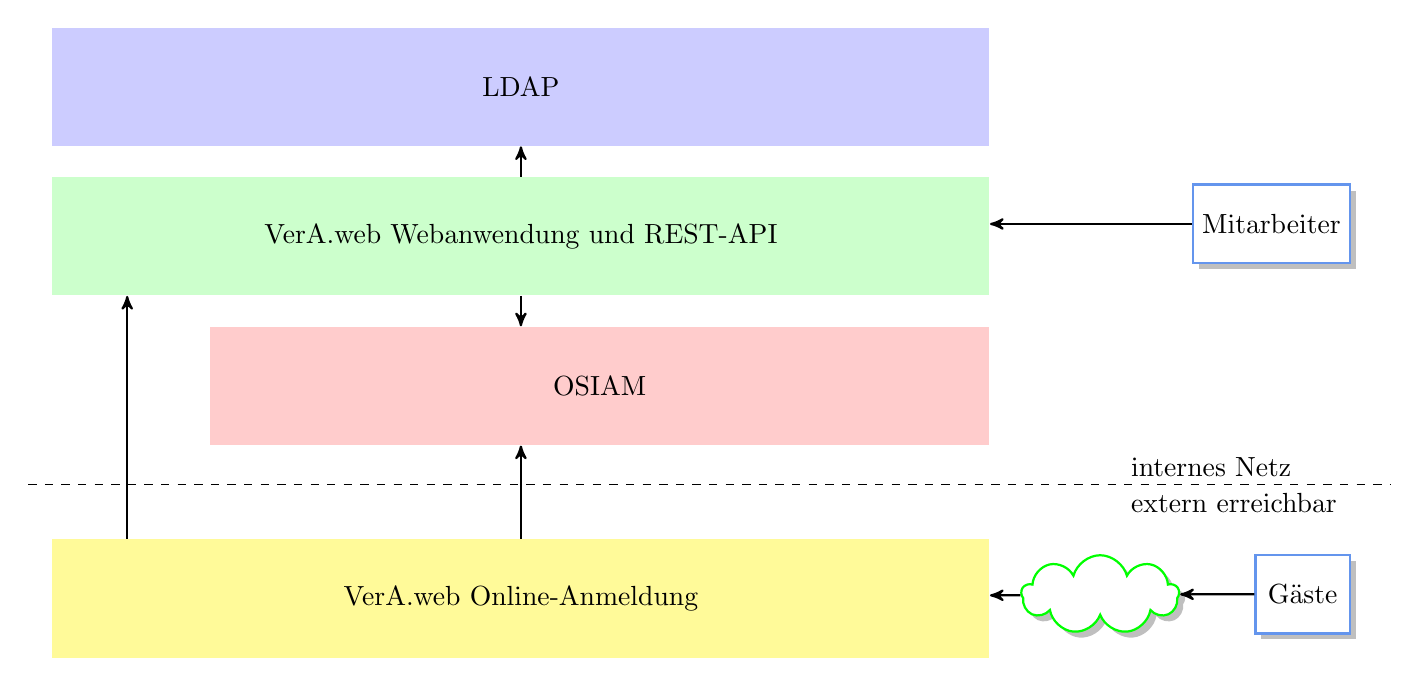
\begin{tikzpicture}[
  >=stealth',
  people/.style={thick,text=black,fill=white,drop shadow,minimum height=10mm,above left,rectangle,draw=CornflowerBlue,minimum width=12mm},
  acloud/.style={thick,text=black,fill=white,drop shadow,cloud,cloud puffs=9,draw=green,above right,minimum width=20mm,minimum height=10mm},
 ]

% \draw (0mm,0mm) -- (0mm,120mm) -- (173mm,120mm) -- (173mm,0mm) -- (0mm,0mm);

  \node[above right,rectangle,fill=blue!20,minimum width=119mm,minimum height=15mm] (ldap) at (3mm,75mm) {LDAP};
  \node[above right,rectangle,fill=green!20,minimum width=119mm,minimum height=15mm] (web) at (3mm,56mm) {VerA.web Webanwendung und REST-API};
  \node[above right,rectangle,fill=yellow!40,minimum width=119mm,minimum height=15mm] (oa) at (3mm,10mm) {VerA.web Online-Anmeldung};
  \node[above right,rectangle,fill=red!20,minimum width=99mm,minimum height=15mm] (osiam) at (23mm,37mm) {OSIAM};

  \node[people]   (sb)     at (168mm,60mm) {Mitarbeiter};
  \node[people]   (guests) at (168mm,13mm) {Gäste};
  \node[acloud]   (inet)   at (130mm,15mm) {};

  \draw[thick,->] (web) -- (ldap);
  \draw[thick,->] (sb.west) -- (sb-|web.east);
  \draw[thick,->] (web.south) -- (web|-osiam.north);
  \draw[thick,->] (guests) -- (inet);
  \draw[thick,->] (inet) -- (oa);
  \draw[thick,->] ([xshift=-5cm]oa.north) -- ([xshift=-5cm]oa|-web.south);
  \draw[thick,->] (oa.north) -- (oa|-osiam.south);

  \node[above right,inner sep=0pt] at (140mm,33mm) {internes Netz};
  \node[below right,inner sep=0pt] at (140mm,31mm) {extern erreichbar};
  \draw[dashed]   (0mm,32mm) -- (173mm,32mm);

\end{tikzpicture}
\end{minipage}

\vspace{10mm}

Falls Sie VerA.web ohne die optionale Online-Anmeldung installieren
gilt das folgende vereinfachte Diagramm:\keinumbruch

\begin{minipage}{\linewidth}
\vspace{5mm}
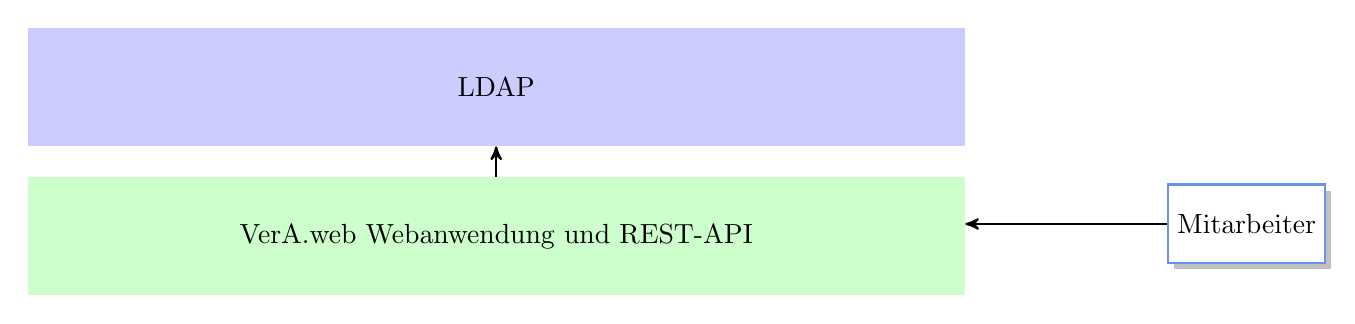
\begin{tikzpicture}[
  >=stealth',
  people/.style={thick,text=black,fill=white,drop shadow,minimum height=10mm,above left,rectangle,draw=CornflowerBlue,minimum width=12mm},
 ]

  \node[above right,rectangle,fill=blue!20,minimum width=119mm,minimum height=15mm] (ldap) at (3mm,23mm) {LDAP};
  \node[above right,rectangle,fill=green!20,minimum width=119mm,minimum height=15mm] (web) at (3mm,4mm) {VerA.web Webanwendung und REST-API};

  \node[people]   (sb)     at (168mm,8mm) {Mitarbeiter};

  \draw[thick,->] (web) -- (ldap);
  \draw[thick,->] (sb.west) -- (sb-|web.east);

\end{tikzpicture}
\end{minipage}

\vspace{5mm}

Auch im folgenden gilt die jeweils vereinfachte Darstellung,
die aus Platzgründen nicht jedes Mal neu abgespalten wird.

\subsection{Die Rolle der REST-API}\label{subsec:intro-restapi}

Die Aufrufe der REST-API werden durch HTTP Basic Authentication mit einem
(Maschinen‑)Benutzernamen und Paßwort gesichert, welche bei den aufrufenden
Anwendungen (der Veranstaltungsmanagementsoftware und, sofern vorhanden, der
Online-Anmeldung) hinterlegt wird; die REST-API wird niemals direkt durch
einen Menschen bedient. Es wird standardmäßig der Benutzer \texttt{veraweb}
mit dem Paßwort \texttt{veraweb} verwendet; eine Änderung der Zugangsdaten
ist \emph{dringend empfohlen}, um die Betriebssicherheit zu gewährleisten;
an den entsprechenden Stellen in dieser Anleitung finden Sie Hinweise hierzu.

\subsection{Detailübersicht}\label{subsec:intro-overview-coarse}

In der nächsten Graphik werden die zu einer vollen Installation (mit allen
optionalen Komponenten und deren Abhängigkeiten) von VerA.web gehörenden
Komponenten mit mehr Detailtiefe aufgeschlüsselt:\keinumbruch

\begin{minipage}{\linewidth}

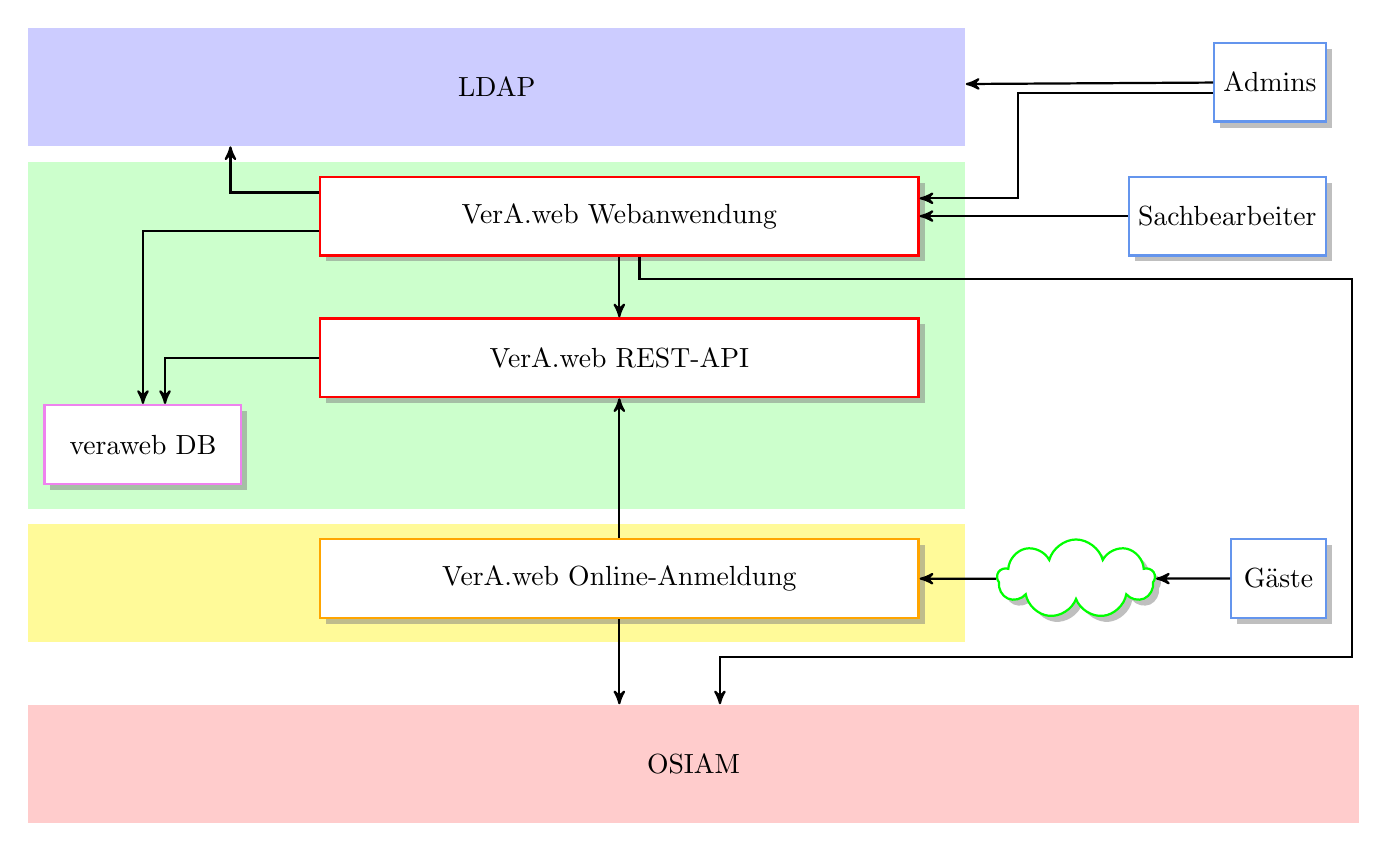
\begin{tikzpicture}[
  >=stealth',
  microsvc/.style={thick,text=black,fill=white,drop shadow,minimum height=10mm,above right,rectangle,draw=Orange,minimum width=76mm},
  webapp/.style={thick,text=black,fill=white,drop shadow,minimum height=10mm,above right,rectangle,draw=red,minimum width=76mm},
  syssvc/.style={thick,text=black,fill=white,drop shadow,minimum height=10mm,above right,rectangle,draw=Violet,minimum width=25mm},
  scrptr/.style={thick,text=black,fill=white,drop shadow,minimum height=10mm,above right,rectangle,draw=black,minimum width=25mm},
  scrptl/.style={thick,text=black,fill=white,drop shadow,minimum height=10mm,above left,rectangle,draw=black,minimum width=25mm},
  people/.style={thick,text=black,fill=white,drop shadow,minimum height=10mm,above left,rectangle,draw=CornflowerBlue,minimum width=12mm},
  acloud/.style={thick,text=black,fill=white,drop shadow,cloud,cloud puffs=9,draw=green,above right,minimum width=20mm,minimum height=10mm},
 ]

% \draw (0mm,0mm) -- (0mm,120mm) -- (173mm,120mm) -- (173mm,0mm) -- (0mm,0mm);

  \fill[yellow!40] (2mm,33mm) -- (121mm,33mm) -- (121mm,48mm) -- (2mm,48mm);
  \fill[green!20] (2mm,50mm) -- (121mm,50mm) -- (121mm,94mm) -- (2mm,94mm);

  \node[above right,rectangle,fill=blue!20,minimum width=119mm,minimum height=15mm] (ldap) at (2mm,96mm) {LDAP};
  \node[above right,rectangle,fill=red!20,minimum width=169mm,minimum height=15mm] (osiam) at (2mm,10mm) {OSIAM};

  \node[microsvc] (svwoa)  at ( 39mm,36mm) {VerA.web Online-Anmeldung};
  \node[webapp]   (score)  at ( 39mm,82mm) {VerA.web Webanwendung};
  \node[webapp]   (svwor)  at ( 39mm,64mm) {VerA.web REST-API};
  \node[syssvc]   (dbvw)   at (  4mm,53mm) {veraweb DB};
  \node[people]   (admins) at (167mm,99mm) {Admins};
  \node[people]   (sb)     at (167mm,82mm) {Sachbearbeiter};
  \node[people]   (guests) at (167mm,36mm) {Gäste};
  \node[acloud]   (inet)   at (129mm,38mm) {};

  \draw[thick,->] (admins) -- ([yshift=3mm]ldap);
  \draw[thick,->] ([yshift=-6mm]admins) -| +(-32mm,0mm) |- ([yshift=3mm]score);
  \draw[thick,->] ([yshift=3mm]score.west) -| ([xshift=-60mm]ldap);
  \draw[thick,->] (sb) -- (score);
  \draw[thick,->] ([yshift=-3mm]score) -| (dbvw);
  \draw[thick,->] ([xshift=4mm]score) |- ++(89mm,-8mm) |- ++(-20mm,-48mm) -| ([xshift=6mm]osiam);
  \draw[thick,->] (score.south) -- (score|-svwor.north);
  \draw[thick,->] (guests) -- (inet);
  \draw[thick,->] (inet) -- (svwoa);
  \draw[thick,->] (svwoa) -- (svwor);
  \draw[thick,->] (svwor) -| ([xshift=6mm]dbvw);
  \draw[thick,->] (svwoa.south) -- (svwoa|-osiam.north);

\end{tikzpicture}

{\footnotesize Zugang für Gäste via DMZ durch das Internet (Wolke);
 Administratoren und Sachbearbeiter via Intranet/VPN}

\end{minipage}

Auch in dieser Abbildung werden LDAP und OSIAM als Blackbox
dargestellt. Um Verwirrung zu vermeiden muß aber bereits hier
erwähnt werden, daß sowohl der LDAP-Server als auch OSIAM ihre
eigene Datenhaltung betreiben \dash die LDAP-Datenbank für slapd
(der OpenLDAP-Server), und eine separate PostgreSQL-Datenbank
für OSIAM.

\subsection{Apache als Frontend}\label{subsec:intro-apache}

Wir empfehlen üblicherweise, alle Systeme aus Sicherheitsgründen so
aufzusetzen, daß HTTPS-Verbindungen im Apache Webserver terminiert
werden und von diesem an die einzelnen Anwendungsserver (über das
AJP-Protokoll an Tomcat und als HTTP-Proxy an den Microservice der
Online-Anmeldung) weitergereicht werden. Sämtliche SSL/TLS-Keys, ‑Features
und weitere sicherheitsrelevante Einstellungen werden im Apache Webserver
eingerichtet, auch um die Angriffsoberfläche zu reduzieren und besser
getesteten und weiter verbreiteten Code zu verwenden, und weil die
Administration der genannten Features in Apache bekannter und erprobter
ist als in den individuellen Anwendungsservern. Sie \emph{können} die
Dienste auch direkt über HTTP ansprechen oder SSL in Java terminieren,
dies widerspricht jedoch unserem empfohlenen Setup und kann nicht, z.B.
im Rahmen dieser Anleitung, unterstützt werden.

Es wird je eine Installation des Webservers pro VM benötigt, da in
der von uns empfohlenen Installationsmethode die Komponenten auch
untereinander ausschließlich verschlüsselt und sicher über HTTPS
miteinander kommunizieren.

\subsection{Komponentendiagramm}\label{subsec:intro-overview-fine}

In dieser Darstellung schlüsseln wir die verwendeten Komponenten
detailliert auf. In der linken Spalte finden Sie Systemdienste
(LDAP, Mailserver) und PostgreSQL-Datenbanken, in der zweiten
Spalte finden Sie die eigentlichen Dienste, in der dritten Spalte
die zugehörigen Apache-Frontends, und in der vierten Spalte die
Benutzer. In schwarzen Kästen befinden sich jeweils zugehörige
Skripte.

\begin{minipage}{\linewidth}

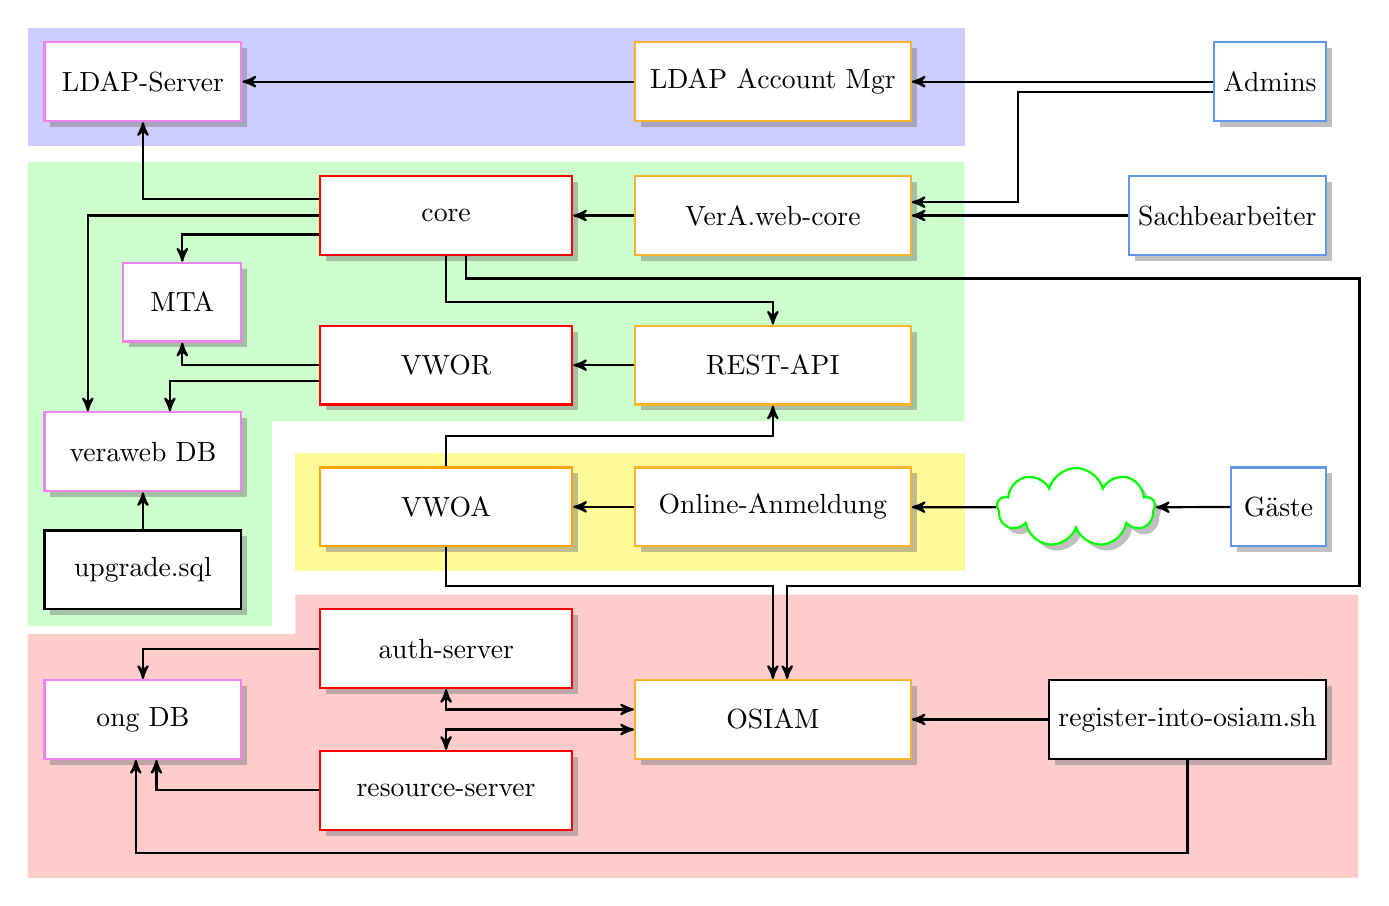
\begin{tikzpicture}[
  >=stealth',
  every node/.style={thick,text=black,fill=white,drop shadow},
  every rectangle node/.style={minimum height=10mm},
  apache/.style={above right,rectangle,draw=Dandelion,minimum width=35mm},
  microsvc/.style={above right,rectangle,draw=Orange,minimum width=32mm},
  webapp/.style={above right,rectangle,draw=red,minimum width=32mm},
  syssvc/.style={above right,rectangle,draw=Violet,minimum width=25mm},
  sysmta/.style={above right,rectangle,draw=Violet,minimum width=15mm},
  scrptr/.style={above right,rectangle,draw=black,minimum width=25mm},
  scrptl/.style={above left,rectangle,draw=black,minimum width=25mm},
  people/.style={above left,rectangle,draw=CornflowerBlue,minimum width=12mm},
  acloud/.style={cloud,cloud puffs=9,draw=green,above right,minimum width=20mm,minimum height=10mm},
 ]

% \draw (0mm,0mm) -- (0mm,120mm) -- (173mm,120mm) -- (173mm,0mm) -- (0mm,0mm);

  \fill[red!20] (2mm,3mm) -- (171mm,3mm) -- (171mm,39mm) -- (36mm,39mm) -- (36mm,34mm) -- (2mm,34mm);
  \fill[yellow!40] (36mm,42mm) -- (121mm,42mm) -- (121mm,57mm) -- (36mm,57mm);
  \fill[green!20] (2mm,35mm) -- (33mm,35mm) -- (33mm,61mm) -- (121mm,61mm) -- (121mm,94mm) -- (2mm,94mm);
  \fill[blue!20] (2mm,96mm) -- (121mm,96mm) -- (121mm,111mm) -- (2mm,111mm);

  \node[apache]   (alam)   at ( 79mm,99mm) {LDAP Account Mgr};
  \node[apache]   (acore)  at ( 79mm,82mm) {VerA.web-core};
  \node[apache]   (avwor)  at ( 79mm,63mm) {REST-API};
  \node[apache]   (avwoa)  at ( 79mm,45mm) {Online-Anmeldung};
  \node[apache]   (aosiam) at ( 79mm,18mm) {OSIAM};
  \node[microsvc] (svwoa)  at ( 39mm,45mm) {VWOA};
  \node[webapp]   (score)  at ( 39mm,82mm) {core};
  \node[webapp]   (svwor)  at ( 39mm,63mm) {VWOR};
  \node[webapp]   (sauth)  at ( 39mm,27mm) {auth-server};
  \node[webapp]   (srsrc)  at ( 39mm, 9mm) {resource-server};
  \node[syssvc]   (ldap)   at (  4mm,99mm) {LDAP-Server};
  \node[syssvc]   (dbvw)   at (  4mm,52mm) {veraweb DB};
  \node[syssvc]   (dbong)  at (  4mm,18mm) {ong DB};
  \node[sysmta]   (mta)    at ( 14mm,71mm) {MTA};
  \node[scrptr]   (usql)   at (  4mm,37mm) {upgrade.sql};
  \node[scrptl]   (riosh)  at (167mm,18mm) {register-into-osiam.sh};
  \node[people]   (admins) at (167mm,99mm) {Admins};
  \node[people]   (sb)     at (167mm,82mm) {Sachbearbeiter};
  \node[people]   (guests) at (167mm,45mm) {Gäste};
  \node[acloud]   (inet)   at (129mm,47mm) {};

  \draw[thick,->] (admins) -- ([yshift=3mm]alam);
  \draw[thick,->] (alam) -- (ldap);
  \draw[thick,->] ([yshift=-6mm]admins) -| +(-32mm,0mm) |- ([yshift=3mm]acore);
  \draw[thick,->] (acore) -- (score);
  \draw[thick,->] ([yshift=5mm]score) -| (ldap);
  \draw[thick,->] (sb) -- (acore);
  \draw[thick,->] (score) -| ([xshift=-7mm]dbvw.north);
  \draw[thick,->] ([yshift=-5mm]score) -| (mta);
  \draw[thick,->] (svwor) -| (mta);
  \draw[thick,->] ([xshift=4mm]score) |- ++(112mm,-8mm) |- ++(-20mm,-39mm) -| ([xshift=6mm]aosiam);
  \draw[thick,->] (score) |- +(25mm,-11mm) -| (avwor);
  \draw[thick,->] (guests) -- (inet);
  \draw[thick,->] (inet) -- (avwoa);
  \draw[thick,->] (avwoa) -- (svwoa);
  \draw[thick,->] (svwoa) |- +(25mm,9mm) -| (avwor);
  \draw[thick,->] (avwor) -- (svwor);
  \draw[thick,->] ([yshift=-4mm]svwor) -| ([xshift=6mm]dbvw);
  \draw[thick,->] (usql) -- (dbvw);
  \draw[thick,<->] ([yshift=3mm]aosiam) -| (sauth);
  \draw[thick,<->] ([yshift=-3mm]aosiam) -| (srsrc);
  \draw[thick,->] (sauth) -| (dbong);
  \draw[thick,->] (srsrc) -| ([xshift=3mm]dbong);
  \draw[thick,->] (riosh) -- +(0mm,-17mm) -| ([xshift=-3mm]dbong);
  \draw[thick,->] (riosh) -- (aosiam);
  \draw[thick,->] (svwoa) |- +(20mm,-10mm) -| (aosiam);

\end{tikzpicture}

\vspace{0.3cm}

\begin{tabu} to \linewidth {rllll}
\rowfont\bfseries\multicolumn{5}{c}{Legende}\\[0.2cm]
 Erste Spalte: & \tikz \node[thick,rectangle,draw=black] {}; Skript &
		 \multicolumn{3}{l}{%
			\tikz \node[thick,rectangle,draw=Violet] {};
			Systemdienst (LDAP, Mailserver,
			PostgreSQL-Datenbank)}\\
Zweite Spalte: & \multicolumn{2}{l}{%
			\tikz \node[thick,rectangle,draw=red] {};
			Webservice (WAR) in Tomcat} &
		 \multicolumn{2}{l}{%
			\tikz \node[thick,rectangle,draw=Orange] {};
			Microservice (JAR)}\\
Dritte Spalte: & \multicolumn{4}{l}{%
			\tikz \node[thick,rectangle,draw=Dandelion] {};
			 Apache Webserver (SSL, mod\_jk oder mod\_proxy\_http)}\\
Vierte Spalte: & \multicolumn{2}{l}{%
			\tikz \node[thick,rectangle,draw=CornflowerBlue] {};
			 Nutzergruppe (per Webbrowser)} &
		 \multicolumn{2}{l}{%
			\tikz \node[thick,rectangle,draw=black] {};
			Skript (Installation/Upgrade)}\\
 Schattierung: & \tikz \node[rectangle,fill=red!30] {}; OSIAM &
		 \tikz \node[rectangle,fill=yellow!60] {}; Online-Anmeldung &
		 \tikz \node[rectangle,fill=green!30] {}; VerA.web core &
		 \tikz \node[rectangle,fill=blue!30] {}; LDAP\\
\multicolumn{5}{l}{\footnotesize
		   Zugang für Gäste via DMZ durch das Internet (Wolke);
		   Administratoren und Sachbearbeiter via Intranet/VPN}\\
\end{tabu}

\end{minipage}

Die WAR‑ und JAR-Dateien aus der zweiten Spalte finden Sie im
nächsten Abschnitt als individuelle Einträge (bzw. bei OSIAM
im entsprechenden Kapitel direkt als Download). Die schwarz
umrahmten Skripte befinden sich im \texttt{files}-Tarball.

\subsubsection{Die OSIAM-Distribution}\label{subsubsec:intro-distro-ong}

Falls Sie während des Aufsetzens von VerA.web eine eigene Installation
von OSIAM einrichten möchten benötigen Sie hierfür auf dem System, auf
dem OSIAM installiert werden soll, Internetzugang, da die notwendigen
Installationspakete (vgl. Kapitel \ref{subsubsec:setup-osiam-download} und
\ref{sec:upgrade-osiam}) „live“ über HTTPS heruntergeladen werden. Nach
erfolgtem Download der Installationspakete während einer Erstinstallation
oder eines Upgrades von OSIAM ist dieser Zugriff selbstverständlich nicht
mehr nötig.

OSIAM ist \emph{nicht} Teil des Veranstaltungsmanagements VerA.web sondern
eine separate Software, die durch VerA.web lediglich verwendet wird, daher
ist OSIAM ebensowenig Teil der VerA.web-Distribution wie zum Beispiel ein
Mailserver oder ein LDAP-Server.

\subsection{Die VerA.web-Distribution}\label{subsec:intro-distro}

Zur Installation bzw. Upgrade müssen Sie folgende Dateien („die
VerA.web-Distribution“) von tarent beziehen:\keinumbruch

\begin{itemize}
 \item{\texttt{veraweb-core-\vwiaverssw{}-files.tgz}}
 \item{\texttt{veraweb-core-\vwiaverssw{}.war}}
 \item{\texttt{rest-api-\vwiaverssw{}.war}}
 \item{\texttt{online-anmeldung-\vwiaverssw{}.jar} (falls gewünscht)}
\end{itemize}

Bitte wenden Sie sich hierzu an unseren Produktvertrieb.

\subsection{Installationsvorgehen}\label{subsec:intro-install}

Installation und Upgrade von VerA.web funktionieren, indem
zunächst Teile der Distribution (siehe oben) auf den Server
kopiert werden, und alle weiteren Schritte dann auf dem System
stattfinden. Die Beispiele sind so gehalten, daß die gesamte
Installation als normaler Benutzer oder \texttt{root} auf dem
jeweiligen
Server durchgeführt werden kann, und privilegierte Operationen
mit Hilfe des Programms \texttt{sudo} durchgeführt werden.

Die weiteren Schritte, die auf dem Server durchzuführen sind,
involvieren:\keinumbruch

\begin{itemize}
 \item{Entpacken der \texttt{files}-Archive}
 \item{Wechseln in ein spezifisches Unterverzeichnis \dash
  alle weiteren Schritte nehmen an, daß dieses Unterverzeichnis
  Ihr aktuelles Arbeitsverzeichnis ist; sollten Sie zwischendurch
  das Verzeichnis wechseln müssen, wechseln Sie einfach zurück,
  bevor Sie den jeweils nächsten Schritt angehen.}
 \item{Anpassen von (Konfigurations‑)Dateien}
 \item{Installation von Dateien und Neustart von Diensten}
 \item{Löschen der ausgepackten Dateien und Installationsarchive}
\end{itemize}

Bei einem Upgrade möchten Sie ggfs. vorher eine Sicherung erstellen.

\subsection{Exkurs: Dienste verwalten mit DJB daemontools}\label{subsec:intro-svc}

Die VerA.web Online-Anmeldung wird als sogenannter Microservice
ausgeführt, im Gegensatz zu den anderen Komponenten, die als
Webarchive in einem Java-Applikationsserver laufen. Ein Microservice
ist hier im wesentlichen ein Java-Archiv (\texttt{*.jar}), das einen
„\texttt{main}“-Einsprungspunkt hat (ähnlich einem C-Programm) und ab
da selbständig lauffähig ist und seinen eigenen Server mitbringt. Er
wird also zum Beispiel von Hand gestartet, indem man einfach dem JRE
sagt „führ mal diesen Code aus“, und schreibt seine Logs auf die
Standardausgabe.

Dies paßt natürlich nicht ins Dienstekonzept von normalen Distributionen,
die für alle Dienste Initskripte mitliefern, mithilfe derer sie gestartet,
gestoppt, ihr Status geprüft, usw. werden können und im Hintergrund laufen.
Als Abhilfe nutzen wir die sogenannten dæmontools von DJB (Professor Daniel
J. Bernstein), die exakt dem Zweck dienen, von Hand gestartete und im
Vordergrund laufende Prozesse in Dienste zu überführen. Als hilfreichen
Nebeneffekt starten die dæmontools einen abgestürzten Dienst automatisch neu.

Dies bedingt natürlich neuer Tools. In Debian haben wir Initskripte in
\texttt{/etc/init.d} \dash zum Beispiel \texttt{/etc/init.d/ssh} \dash
und in manchen neueren Installationen systemd-Units \dash zum Beispiel
\texttt{/lib/systemd/system/ssh.service} \dash welche alle Informationen
enthalten, die einen Dienst ausmachen. Über den Basisnamen, in unserem
Beispiel \texttt{ssh}, kann man den Dienst steuern: \texttt{sudo service
ssh start}, oder stop, oder status.

In DJB dæmontools werden die Informationen zu Diensten, und manchmal auch
die Logs und/oder die Programme selber, als Verzeichnisse unterhalb von
\texttt{/service}\Hair\footnote{in Debian \texttt{/etc/service}, um dem
Dateisystemhierarchiestandard zu genügen, aber ein Symlink, der von
\texttt{/service} nach \texttt{/etc/service} zeigt, ist schnell gesetzt
und Teil unserer Installationsanleitung} abgelegt. So befinden sich die
Informationen der VerA.web Online-Anmeldung unter \texttt{/service/vwoa/}.

Die Nutzung des Verzeichnisses \texttt{/service} ist ein Standard und
Konsens, und nur Dienste, die dort abgelegt werden, werden beim Systemstart
automatisch gestartet, aber grundsätzlich verwenden die dæmontools immer
den vollen Pfad, und so könnte man auch andere Verzeichnisse verwenden.
Aber unser Ziel hier ist ja, ein rebootfestes System einzurichten.

Beginnen wir mit \texttt{sudo svstat /service/vwoa/} \dash dieser Befehl
zeigt uns an, ob der Service läuft (\texttt{up}) oder nicht (\texttt{down});
falls er läuft, welche Prozeß-ID (\texttt{pid}) er besitzt (dies ist für
Sie nicht weiter relevant); wie lange er bereits in diesem Zustand ist,
und, falls der aktuelle Zustand nicht der Standardzustand\Hair\footnote
{wenn Sie eine Datei \texttt{/service/vwoa/down} anlegen wird der Dienst
nicht mehr automatisch gestartet; Sie können ihn dann immer noch manuell
mit \texttt{svc} starten oder den Standardzustand wieder auf \texttt{up}
stellen, indem Sie die Datei \texttt{down} entfernen und rebooten} ist,
ebendies.

Für die eigentliche Verwaltung eines Dienstes gibt es den Befehl
\texttt{svc}. So wird ein Dienst, der \texttt{down} ist, mit dem Befehl
\texttt{sudo svc -u /service/vwoa} gestartet (das \texttt{u} steht für
„\emph{u}p“, also „hochgefahren“).

Wenn der Dienst nicht richtig konfiguriert ist und gar nicht erst hochkommt
wird er danach trotzdem immer wieder neugestartet; Sie sehen das in der
Ausgabe von \texttt{svstat} daran, daß der Dienst zwar \texttt{up} ist,
aber mit einer sehr kleinen Sekundenzahl, die immer wieder auf 0 zurückkehrt.

Sie können einen Dienst, der \texttt{down} ist, auch mit dem Befehl
\texttt{sudo svc -o /service/vwoa} hochfahren \dash das \texttt{o} steht
hier für „\emph{o}nce“, also „einmalig“. Der Dienst wird gestartet; wenn
er läuft bleibt er laufen (bis er sich selber beendet oder abstürzt), und
wenn er nicht startet ist er danach wieder \texttt{down}. Wenn der Dienst
sauber läuft können Sie das Feature des automatischen Neustarts durch ein
einfaches \texttt{sudo svc -u /service/vwoa} auch aktivieren, während er
durch \texttt{svc -o} gestartet wurde.

Um einen Dienst neuzustarten nutzen Sie \texttt{sudo svc -t /service/vwoa}
\dash das \texttt{t} steht für „\emph{t}erminate“, also „beenden“. Ein wenig
seltsam, bis man sich erinnert, daß beendete Dienste automatisch neugestartet
werden (außer sie wurden mit \texttt{svc -o} gestartet), diese Aktion ist
also vielmehr ein Stoppen, auf das implizit der automatische Neustart folgt.

Wenn Sie einen Dienst nun wirklich stoppen wollen benutzen Sie den Befehl
\texttt{sudo svc -d /service/vwoa} \dash \texttt{d} wie „\emph{d}own“, also
„heruntergefahren“. Beachten Sie aber, daß der Dienst beim nächsten Reboot
automatisch wieder gestartet wird, solange keine Datei (kann auch leer sein)
\texttt{/service/vwoa/down} existiert.

\texttt{man svc} zeigt noch einige weitere Optionen, aber die hier erwähnten
sind die, die ein Systemadministrator im normalen Betrieb benötigt.

\subsection{Exkurs: Wechsel von systemd nach sysvinit}\label{subsec:intro-sysvinit}

Eine Standardinstallation (kein Upgrade) von Debian 8 „jessie“ oder neuer
benutzt \texttt{systemd} als Init-System. Wir haben unsere Software und
insbesondere die Integration der Online-Anmeldung jedoch ausschließlich
mit \texttt{sysvinit}, das Unix-Administratoren vertrauter ist, getestet.

\begin{minipage}{\linewidth}
Zum Wechsel führen Sie folgenden Befehl aus:

\begin{lstdump}{sysvinit installieren}
sudo apt-get install sysvinit-core
\end{lstdump}

Danach rebooten Sie das System. Prüfen Sie dann, welches \texttt{init} läuft:

\begin{lstdump}{init herausfinden}
sudo ls -l /proc/1/exe
\end{lstdump}

Wenn hinter dem „Pfeil“ \texttt{->} in der Ausgabe der Text
\texttt{/lib/systemd/systemd} steht war der Vorgang nicht
erfolgreich; bei \texttt{/sbin/init} stimmt alles, und Sie
können, falls Sie möchten (dies ist nicht zur Benutzung von
VerA.web notwendig), nun \texttt{systemd} ganz entfernen:

\begin{lstdump}{systemd entfernen}
sudo apt-get purge --auto-remove systemd
\end{lstdump}
\end{minipage}

Einer Nutzung von VerA.web unter \texttt{systemd} steht
nichts Grundsätzliches im Wege; es sprengt lediglich den
aktuellen Rahmen dieser Anleitung und erschwert die
Nutzung von daemontools (siehe voriges Kapitel), welches
zum Aufsetzen der Online-Anmeldung benutzt wird.

\section{Systemvoraussetzungen}\label{sec:requirements}

In der Angabe für den benötigten Festplattenplatz ist die
Grundinstallation des Betriebssystems (ohne Auslagerungsdatei)
einkalkuliert.

Die Systemvoraussetzungen unterscheiden sich je nachdem wie Sie die
Komponenten auf individuelle VMs verteilen. Im folgenden werden im
wesentlichen die Werte für zwei verschiedene Szenarien angegeben:
core und OSIAM auf separaten Systemen (oder keine Online-Anmeldung)
oder zusammen auf einem System. Die Online-Anmeldung selbst wird
als separates System geführt; sie kann auch mit dem core-System
zusammengelegt werden, dies erhöht die Anforderungen an dieses nur
minimal.

\begin{tabular}{| r || l | l | l |}\hline
                          & Minimum                & empfohlen     & Maximum\\\hline\hline
 Anzahl Prozessoren je VM & 1                      & 1             & 1\Hair\textsuperscript{\ref{fn:req-tst-notmore}}\\\hline
 Betriebssystem           & Debian 8 („jessie“)    & 9 („stretch“) & unstable\Hair\textsuperscript{\ref{fn:req-nolimit}}\\\hline
 Java™-Laufzeitumgebung   & OpenJDK 8 JRE headless & wie Minimum   & OpenJDK 8\Hair\textsuperscript{\ref{fn:req-nonewer}}\\\hline
 Applikationsserver       & Tomcat 8               & wie Minimum   & Tomcat 8\Hair\textsuperscript{\ref{fn:req-notmore}}\\\hline
 Webserver                & Apache 2.2             & Apache 2.4    & Apache 2.4\Hair\textsuperscript{\ref{fn:req-notmore}}\\\hline
 Datenbank                & PostgreSQL 9.1         & aktuelle 9.x  & PostgreSQL 9.6\Hair\textsuperscript{\ref{fn:req-notmore}}\\\hline
%XXX TODO: PostgreSQL 10+ testen
 OSIAM (alleine) Arbeitsspeicher   &  960 MiB      & 1536 MiB      & 2048 MiB\Hair\textsuperscript{\ref{fn:req-tst-notmore}}\\\hline
 OSIAM (alleine) Festplattengröße  &    2 GB       &    4 GB       &    8 GB\Hair\textsuperscript{\ref{fn:req-tst-notmore}}\\\hline
 core (alleine) Arbeitsspeicher    &  512 MiB      & 1024 MiB      & 2048 MiB\Hair\textsuperscript{\ref{fn:req-tst-notmore}}\\\hline
 core (alleine) Festplattengröße   &    2 GB       &    8 GB       &   20 GB\Hair\textsuperscript{\ref{fn:req-tst-notmore}}\\\hline
 core + OSIAM Arbeitsspeicher      & 1024 MiB      & 2048 MiB      & 4096 MiB\Hair\textsuperscript{\ref{fn:req-tst-notmore}}\\\hline
 core + OSIAM Festplattengröße     &    3 GB       &   10 GB       &   20 GB\Hair\textsuperscript{\ref{fn:req-tst-notmore}}\\\hline
 Online-Anmeldung Arbeitsspeicher  &  512 MiB      &  768 MiB      & 1024 MiB\Hair\textsuperscript{\ref{fn:req-tst-notmore}}\\\hline
 Online-Anmeldung Festplattengröße &    ½ GB       &    3 GB       &    8 GB\Hair\textsuperscript{\ref{fn:req-tst-notmore}}\\\hline
\end{tabular}

Bitte beachten Sie bei der Dimensionierung der Maschinen und der
Netzwerkanbindung, daß das Veranstaltungsmanagement (core) nur
durch Ihre Mitarbeiter bedient wird, während die Online-Anmeldung
üblicherweise offen im Internet steht und entsprechender Last
ausgesetzt sein \emph{kann}.

\hyperfootnotetext{\label{fn:req-tst-notmore}%
 wir haben keine größere Konfiguration getestet; eine praktische
 Obergrenze anzugeben ist jedoch unrealistisch}%
\hyperfootnotetext{\label{fn:req-nolimit}%
 keine praktische Begrenzung}%
\hyperfootnotetext{\label{fn:req-nonewer}%
 neuere Versionen funktionieren \emph{nicht}!}%
\hyperfootnotetext{\label{fn:req-notmore}%
 neuere Versionen wurden nicht getestet oder existierten zum
 Testzeitpunkt nicht}%

\subsection{LDAP-Verzeichnisdienst}\label{subsec:req-ldap}

Sie benötigen ein LDAP-Verzeichnis, in dem Sie die Zugänge (user
accounts) für die Sachbearbeiter, die VerA.web benutzen sollen,
sowie Administratorenzugänge pflegen.

VerA.web hat keine eigene Benutzerverwaltung sondern fragt beim
Login eines Nutzers das LDAP-Verzeichnis ab, ob die Kombination
aus Benutzernamen und Paßwort gültig ist. Nur die Zuordnung von
Benutzern (identifiziert durch den Unix-Benutzernamen bzw. die
\texttt{uid}) zu Benutzerrechten (z.B. Administrator oder Lesen
eingeschränkt) und Mandanten wird durch VerA.web gespeichert;
Näheres finden Sie in Kapitel 6.2 (Administration > Benutzer)
im \href%
{https://evolvis.org/plugins/scmgit/cgi-bin/gitweb.cgi?p=veraweb/veraweb.git;a=blob_plain;f=vwor/src/main/webapp/doc/Benutzerhandbuch.pdf;hb=HEAD#6.2 Benutzer}%
{VerA.web-Benutzerhandbuch}. Einige weitere LDAP-Attribute wie
\texttt{givenName} und \texttt{sn} (Vor‑ und Zuname) werden
ebenfalls verwendet, sowie \texttt{mail} als Absendeadresse beim
Versand von eMails.

Für eine kleine Site ist es möglich, den LDAP-Server (Debian-Pakete
\texttt{slapd} (OpenLDAP-Server) und \texttt{ldap-utils} sowie, als
einfach bedienbare Oberfläche, \texttt{ldap-account-manager}) auf
demselben Server wie die interne Veranstaltungs- und Adreßverwaltung
laufenzulassen; dies erhöht die Systemvoraussetzungen nicht nennenswert.
Alle Informationen hierzu finden Sie in Kapitel \ref{sec:setup-lam}.

\subsection{Interne Veranstaltungs- und Adreßverwaltung}\label{subsec:req-core}

Zum Betrieb von VerA.web core empfehlen wir eine eigenständige VM
(OSIAM kann auf dem System mitinstalliert werden, wenn es nur für
VerA.web verwendet wird) mit der stabilen Debian-Version 9 („stretch“)
als Betriebssystem. Zwar \emph{kann} die Software auch mit einer
anderen Debian-basierten Distribution (z.B. Ubuntu) oder einer
anderen Java/Tomcat-Umgebung (z.B. Solaris) betrieben werden,
allerdings geht diese Installationsanleitung von der empfohlenen
Systemumgebung aus. Eine graphische Oberfläche auf dem Server wird
zum Betrieb nicht benötigt.

Falls Sie abweichende Konfigurationen benutzen müssen Sie ggfs.
Pfade (z.B. \texttt{/usr/ucb/install} statt einfach \texttt{install}),
Befehle (z.B. \texttt{zcat … | tar -xf -} statt \texttt{tar -xzf …}),
u.ä. an die modifizierte Umgebung anpassen.

In dieser Anleitung sowie den Systemvoraussetzungen wird weiterhin
angenommen, daß der notwendige Datenbankserver (PostgreSQL) auf
derselben VM wie die interne Veranstaltungs- und Adreßverwaltung läuft;
falls nicht ändern Sie bitte an den relevanten Stellen den Hostnamen,
ggfs. Port, und Datenbanknamen in den Konfigurationsdateien.
Der PostgreSQL-Datenbankserver für OSIAM \emph{muß} hingegen aus Gründen
der Einfachheit auf demselben System wie der OSIAM-Anwendungsserver laufen.

Desweiteren benötigen Sie den Applikationsserver Tomcat 8 mit einer
Java™-Laufzeitumgebung (OpenJDK) ab Version 8, ohne GUI (headless JRE),
sowie den Webserver Apache 2 mit \texttt{mod\_proxy\_http} (nur bei
Verwendung der optionalen Online-Anmeldung), \texttt{mod\_jk} und SSL.

⚠ \emph{Achtung:} Java™ 7 oder älter sowie Tomcat 7 oder älter werden
nicht unterstützt und führen während der Installation zu Fehlern!

\subsubsection{Mailserver (MTA)}\label{subsubsec:req-core-mta}

Auf dem Server für VerA.web core und REST-API \emph{muß} ein
Mailserver (z.B. \texttt{postfix} oder \texttt{sendmail} aus Debian)
installiert sein, der lokale Verbindungen auf Port 25 entgegennimmt
und die eingehenden Nachrichten, ggfs. über einen als Smarthost
eingestellten anderen Mailserver, zustellt.

\subsection{Online-Anmeldung}\label{subseq:req-oa}

Zum Betrieb der Online-Anmeldung empfehlen wir ebenfalls eine
eigenständige VM; sie kann allerdings auch auf demselben System
wie der VerA.web core eingerichtet werden. Auch hier wird eine
Installation von Debian 9 „stretch“ ohne graphische Oberfläche
und mit \texttt{sysvinit} vorausgesetzt.

Die Online-Anmeldung hat relativ bescheidene Voraussetzungen
und kann bereits mit 512 MiB Arbeitsspeicher und 1½ GB Festplatte
betrieben werden; die Werte steigen je nach Auslastung entsprechend.

Auch hier benötigen Sie den Apache Webserver und die Java™ 8
Laufzeitumgebung, allerdings keinen Tomcat-Applikationsserver, da
die Online-Anmeldung als sogenannter Microservice implementiert wurde.

\subsection{Bevor Sie beginnen}\label{subsec:req-prereq}

Im Verlauf der Installation werden Sie mindestens einen Useraccount
in VerA.web als Administrator anlegen. Hierfür informieren Sie sich
bitte vorab über die LDAP-Kürzel (Unix-Loginnamen, üblicherweise das
Attribut \texttt{uid}) des oder der Benutzer, der/die initial als
VerA.web-Administratoren dienen sollen.

Plazieren Sie bitte auf jeder VM das zugehörige SSL-Zertifikat als
\texttt{/etc/ssl/vwserver.cer}, den privaten Schlüssel als
\texttt{/etc/ssl/private/vwserver.key}, und, sofern vorhanden, die
Zertifikatskette als \texttt{/etc/ssl/vwchain.cer}. Setzen Sie die
Rechte entsprechend:\keinumbruch

\begin{minipage}{\linewidth}
\begin{lstdump}{SSL-Zertifikate}
sudo chown 0:ssl-cert /etc/ssl/vw*.cer /etc/ssl/private/vwserver.key
sudo chmod 644 /etc/ssl/vw*.cer
sudo chmod 640 /etc/ssl/private/vwserver.key
\end{lstdump}
\end{minipage}

Unsere Software wird ausschließlich auf normalen Linux-Systemen ohne
SELinux getestet. Sollten Sie eine Distribution mit SELinux einsetzen
müssen Sie SELinux deaktivieren, zum Beispiel kurzzeitig (bis spätestens
zum nächsten Neustart) mit dem Befehl \texttt{sudo setenforce 0}, oder,
z.B. auf RHEL und CentOS, permanent, indem Sie in der Konfigurationsdatei
\texttt{/etc/sysconfig/selinux} die Einstellung \texttt{SELINUX=disabled}
setzen und das System neustarten.

\section{Installation OpenLDAP und LDAP-Account-Manager}\label{sec:setup-lam}

Falls Sie bereits über einen \nameref{subsec:req-ldap} verfügen
überspringen Sie dieses Kapitel bitte und lesen Sie direkt in
Kapitel \nameref{sec:setup-osiam} weiter.

Diese Installation wird üblicherweise auf dem Server durchgeführt,
auf dem Sie später auch VerA.web-core installieren möchten.

\subsection{Installation OpenLDAP-Server}\label{subsec:setup-lam-slapd}

\begin{minipage}{\linewidth}
Installieren Sie zunächst die nötigen Pakete:

\begin{lstdump}{Install LDAP}
sudo apt-get install slapd ldap-utils ldap-account-manager php-xml php-zip
\end{lstdump}

Vergeben Sie ein Administratorpaßwort für das LDAP und merken
Sie sich es gut!
\end{minipage}

In der Datei \texttt{/etc/ldap/slapd.d/cn=config/olcDatabase=\{1\}mdb.ldif}
finden Sie jetzt einen Eintrag \texttt{olcSuffix}. Notieren Sie sich den
Teil hinter dem Doppelpunkt (und Leerzeichen); dies ist Ihr sogenannter
„Base DN“. In dieser Dokumentation wird \texttt{dc=lan,dc=tarent,dc=de} als
Beispiel verwendet.

Führen Sie das folgende kleine Skript aus oder nehmen Sie die Änderungen,
die es durchführt, manuell vor: \texttt{/etc/ldap/ldap.conf} bearbeiten,
indem eine Zeile eingefügt wird, die mit dem Wort \texttt{BASE} in Versalien
beginnt und dann hinter einem Leerzeichen (ohne Doppelpunkt, diesmal) den
Base-DN enthält.\keinumbruch

\begin{minipage}{\linewidth}
\begin{lstdump}{LDAP-Clientkonfiguration}
cfg='/etc/ldap/slapd.d/cn=config/olcDatabase={1}mdb.ldif'
basedn=$(sudo sed -n '/^olcSuffix: */s///p' "$cfg")
echo "Der Base-DN ist: $basedn"
sudo sh -c "echo 'BASE $basedn' >>/etc/ldap/ldap.conf"
\end{lstdump}
\end{minipage}

Danach können Sie mit dem Befehl \texttt{ldapsearch -x} bereits die in
Ihrem neuen LDAP-Verzeichnis enthaltenen Einträge sehen; dies ist initial
lediglich der Wurzelknoten \texttt{dc=lan,dc=tarent,dc=de} sowie der
LDAP-Administrator \texttt{cn=admin,dc=lan,dc=tarent,dc=de}.

\subsection{Konfiguration LDAP-Account-Manager}\label{subsec:setup-lam-cfg}

Nun müssen Sie den LDAP-Account-Manager „lam“ \dash eine Weboberfläche,
die zum vereinfachten Anlegen von Benutzern im LDAP dienen kann \dash
einrichten. Benutzen Sie zu diesem Zweck einen Webbrowser, in dem Sie
das Verzeichnis \texttt{/lam/} auf dem neuen Server aufrufen, also zum
Beispiel \texttt{http://veraweb.lan.tarent.de/lam/} \dash leider läßt
die Einrichtung sich nicht sinnvoll über Konfigurationsdateiänderungen
automatisieren sondern muß manuell mit einem Webbrowser durchgeführt
werden.

Dort klicken Sie zunächst oben rechts auf:
\inlinebild[LAM configuration]{lam-tools}

Unterhalb von \inlinebild[Edit general settings]{lam-tools} finden
Sie, nachdem Sie sich mit dem Master-Paßwort „lam“ authentifiziert
haben, ganz unten auf der Seite die Möglichkeit, ebendieses zu ändern.

Nach dem Speichern wählen Sie wieder:
\inlinebild[LAM configuration]{lam-tools}

Nun finden Sie unter \inlinebild[Edit server profiles]{lam-profiles}
einige weitere Einstellungen. Geben Sie zunächst im dritten Feld
(Tree suffix) Ihren Base DN ein, und unten bei „List of valid users“
unterhalb von \inlinebild[Security settings]{lam-security} den DN
des LDAP-Administrators\Hair\footnote{hier
\texttt{cn=admin,dc=lan,dc=tarent,dc=de} \dash zu sehen mit
\texttt{ldapsearch -x} \dash vgl. Kapitel \ref{subsec:setup-lam-slapd}}.

\strut Sie brauchen an dieser Stelle noch nicht zu speichern. Wählen Sie
oben den Registerreiter \inlinebild[Account types]{lam-gear} aus. Stellen
Sie sicher, daß unter „Active account types“ nur \inlinebild[Users]{lam-user}
und \inlinebild[Groups]{lam-group} gelistet sind, indem Sie neben ggfs.%
\Hair\footnote{\label{fn:vor9}in Debian 9 „stretch“ entspricht dies der
Voreinstellung} weiteren Einträgen rechts das Lösch-Icon \inlinebild{lam-del}
anklicken, um die weitere Verwaltung zu vereinfachen. Ändern Sie dann den
„LDAP suffix“ für \inlinebild[Users]{lam-user} in \texttt{ou=Users} gefolgt
von einem Komma und Ihrem Base DN (\texttt{ou=Users,dc=lan,dc=tarent,dc=de}
in unserem Beispiel), und den „LDAP suffix“ für \inlinebild[Groups]{lam-group}
\strut in \texttt{ou=Group} gefolgt von einem Komma und Ihrem Base DN, also
z.B: \texttt{ou=Group,dc=lan,dc=tarent,dc=de}\strut

\strut Fahren Sie im Registerreiter \inlinebild[Modules]{lam-modules} fort,
indem Sie wieder sicherstellen, daß nur die Module \texttt{inetOrgPerson},
\texttt{posixAccount} und \texttt{shadowAccount} (Users) bzw.\strut
\texttt{posixGroup} (Groups) aktiv sind\Hair\textsuperscript{\ref{fn:vor9}}.
Unter \inlinebild[Module settings]{lam-modules} können Sie, falls\strut
gewünscht, einzelne Felder aus der Anzeige ausblenden, um die spätere
Benutzung weiter zu vereinfachen.\strut

Jetzt können Sie mit \inlinebild[Save]{lam-save} speichern. Dann können\strut
Sie sich auf der nun erscheinenden regulären Loginmaske mit dem Paßwort\strut
des LDAP-Administrators anmelden. Beim ersten Login erscheint eine\strut
Abfrage „The following suffixes are missing in LDAP. LAM can create them
for you.“, welche Sie mit „Create“ bestätigen. Jetzt müssen Sie noch\strut
unter \inlinebild[Groups]{lam-group} eine Gruppe erstellen, der später
alle User standardmäßig zugeordnet werden; klicken Sie hierzu auf\strut
\inlinebild[New group]{lam-add} und geben als „Group name“ einfach\strut
„ldapusers“ an und klicken oben links auf \inlinebild[Save]{lam-save}.

Damit ist die Ersteinrichtung des LDAP-Account-Managers abgeschlossen.

\subsection{LDAP-Nutzer anlegen}\label{subsec:setup-lam-adduser}

Um einen Benutzer im LDAP anzulegen müssen Sie sich ggfs. (außer direkt
nach der Ersteinrichtung) wieder mit dem Paßwort des LDAP-Administrators
anmelden; sonst wählen Sie den Registerreiter \inlinebild[Users]{lam-user}
einfach direkt aus. Klicken Sie dann auf \inlinebild[New user]{lam-add}.

In der folgenden Maske müssen Sie mindestens den „Last Name“ ausfüllen;
die „Email address“ ist zwar keine Pflicht, aber sinnvoll.
Klicken Sie dann links auf \inlinebild[Unix]{lam-tux} und tragen im Feld
„User name“ ein geeignetes Kürzel (⚠ nur Kleinbuchstaben und Zahlen) ein;
mit diesem Kürzel kann sich später der Nutzer bei VerA.web anmelden. Nun
wählen Sie noch \inlinebild[Set password]{lam-key}, tragen das gewünschte
Paßwort für den neu anzulegenden User (in beide Felder) ein, klicken im
Dialog auf „Ok“ und dann oben links wieder auf \inlinebild[Save]{lam-save}.

Jetzt erscheint die Meldung „Account was created successfully.“ in einem
blauen Kasten; damit ist dieser Nutzer angelegt und kann in VerA.web core
freigeschaltet werden, entweder, bei der Erstinstallation, über die
Datenbank (siehe Kapitel \ref{manual:db-user}), oder, später, über die
Weboberfläche (siehe Benutzerhandbuch).

\section{Installation OSIAM-System}\label{sec:setup-osiam}

Dieser Abschnitt gliedert sich in zwei Teile: die generelle Installation
von OSIAM, sofern Sie noch keine laufende OSIAM-Installation haben, und
die Registration der VerA.web Online-Anmeldung beim OSIAM-Server.

Kopieren Sie jedoch bitte zunächst die Datei
\texttt{veraweb-core-\vwiaverssw{}-files.tgz}
auf den OSIAM-Server.

\begin{minipage}{\linewidth}
Entpacken Sie das \texttt{files}-Archiv und wechseln in das
Unterverzeichnis mit den OSIAM-Dateien:

\begin{lstdump}{Entpacken OSIAM}
tar -xzf veraweb-core-〈\lstdumpesc{\vwiaverssw}〉-files.tgz
cd veraweb-core-〈\lstdumpesc{\vwiaverssw}〉/osiam
chmod go-rwx .
\end{lstdump}
\end{minipage}

Alle weiteren Schritte in diesem Kapitel nehmen an, daß dieses
Unterverzeichnis Ihr aktuelles Arbeitsverzeichnis ist.

Der \texttt{chmod}-Aufruf dient dazu, anderen auf demselben System
eingeloggten Nutzern den Zugriff auf die Konfigurationsdateien zu
verweigern während Sie sie bearbeiten, da sie später Paßwörter
enthalten werden.

\subsection{OSIAM-Server Schnellinstallation}\label{subsec:setup-osiam-fast}

VerA.web benötigt aktuell OSIAM auth-server und resource-server in
der Version \vwiaversosiam{} und ist \emph{nur} mit dieser Version
sowie auth-server und resource-server 2.3 aus der OSIAM-Distribution
2.4 (der in vorherigen Fassungen dieser Anwendung empfohlenen und in
den Docker-Images noch verwendeten Version) getestet worden.\keinumbruch

⚠ \emph{Achtung:} Die Version von OSIAM muß die in der jeweils
benutzten VerA.web-Version dokumentierte sein!

Falls Sie bereits eine lauffähige OSIAM-Installation besitzen stellen
Sie bitte sicher, daß auf die vorhandene Installation über HTTPS
zugegriffen werden kann; danach können Sie direkt im nächsten Abschnitt
(\nameref{subsec:setup-osiam-register}) weiterlesen.

\subsubsection{System vorbereiten}\label{subsubsec:setup-osiam-prepare}

\begin{minipage}{\linewidth}
Sofern Sie noch nicht über eine OSIAM-Installation besitzen, bereiten
Sie bitte zunächst das System vor, indem Sie einige Pakete installieren
und sicherstellen, daß keine ältere Java-Version installiert ist bzw.
versehentlich verwendet wird:

\begin{lstdump}{Pakete OSIAM}
sudo apt-get install curl apache2 postgresql openjdk-8-jre-headless \
    tomcat8 libtcnative-1 libservlet3.1-java libapache2-mod-jk
sudo a2dismod mpm_event
sudo a2enmod mpm_prefork
java -version
### sollte etwa ausgeben:
# openjdk version "1.8.0_162"
# OpenJDK Runtime Environment (build 1.8.0_162-8u162-b12-1~deb9u1-b12)
# OpenJDK 64-Bit Server VM (build 25.162-b12, mixed mode)
\end{lstdump}
\end{minipage}

\begin{minipage}{\linewidth}
Kopieren Sie außerdem die Datei \texttt{postgresql-jdbc4.jar} aus
dem „files“-Tarball nach \texttt{/var/lib/tomcat8/lib/} (hierbei
ggfs. bereits existierende überschreiben):

\begin{lstdump}{JDBC OSIAM}
sudo cp ../postgresql-jdbc4.jar /var/lib/tomcat8/lib/
\end{lstdump}
\end{minipage}

Jetzt sind der Datenbankserver, die Java™-Laufzeitumgebung (in der
Version für Server und Webanwendungen), der Tomcat-Applikationsserver,
der Webserver sowie Hilfsprogramme installiert.

\subsubsection{Datenbank}\label{subsubsec:setup-osiam-db}

\begin{minipage}{\linewidth}
Legen Sie den Datenbankbenutzer und die Datenbank an:

\begin{lstdump}{DB erstellen OSIAM}
# createuser fragt nach einem zu vergebenden Paßwort
sudo -u postgres createuser -D -P -R -S ong
sudo -u postgres createdb -E UTF-8 -O ong -T template0 ong
\end{lstdump}

Falls Sie hierbei ein anderes Paßwort als \texttt{ong} für
den Datenbanknutzer vergeben müssen Sie jetzt die Angaben
in den Dateien \texttt{auth-server.properties} und
\texttt{resource-server.properties} entsprechend anpassen.
\end{minipage}

Das Datenbankschema wird durch OSIAM selbst automatisch verwaltet.

\subsubsection{Applikationsserver}\label{subsubsec:setup-osiam-tomcat}

\begin{minipage}{\linewidth}
In den Dateien \texttt{auth-server.properties} und
\texttt{resource-server.properties} ersetzen Sie bitte an allen
Stellen \texttt{HOSTNAME-OSIAM} durch den vollen Hostnamen des
OSIAM-Servers. Danach installieren Sie diese:

\begin{lstdump}{/etc/osiam fuellen}
sudo mkdir -p /etc/osiam
sudo chown 0:tomcat8 /etc/osiam
sudo chmod 2750 /etc/osiam
sudo install -c -o 0 -g tomcat8 -m 640 *.properties /etc/osiam/
sudo mkdir -p /etc/osiam/auth-server/templates/web
\end{lstdump}
\end{minipage}

Fügen Sie bitte am Ende der Datei \texttt{/etc/default/tomcat8}
einige Zeilen ein, um weitere JVM-Startoptionen zu setzen.

\begin{minipage}{\linewidth}
Diese Option setzen Sie bitte in jedem Fall, um eine korrekte
Kodierung von Dateien, Logs und internen Abläufen zu gewährleisten:

\begin{lstdump}{Tomcat Encoding setzen}
JAVA_OPTS="${JAVA_OPTS} -Dfile.encoding=UTF-8"
\end{lstdump}
\end{minipage}

\begin{minipage}{\linewidth}
Diese (Linux-spezifische) Option spart u.a. beim Starten Zeit,
indem sie eine nichtblockierende Quelle für Zufallszahlen auswählt:

\begin{lstdump}{Tomcat /dev/urandom}
JAVA_OPTS="${JAVA_OPTS} -Djava.security.egd=file:/dev/./urandom"
\end{lstdump}
\end{minipage}

\begin{minipage}{\linewidth}
Fügen Sie eine der beiden folgenden Zeilen hinzu:

\begin{lstdump}{Tomcat Speicher}
JAVA_OPTS="${JAVA_OPTS} -Xmx512m"               # bei weniger als 1280 MiB RAM
JAVA_OPTS="${JAVA_OPTS} -Xms512m -Xmx1024m"     # andernfalls
\end{lstdump}
\end{minipage}

\begin{minipage}{\linewidth}
Hängen Sie an die \texttt{/etc/tomcat8/logging.properties} folgende
Zeilen an:

\begin{lstdump}[breaklines=false]{Tomcat Logging}
java.util.logging.SimpleFormatter.format=%1$tF %1$tT.%1$tL %4$7s (%2$s) [%3$s] %5$s%6$s%n
org.apache.juli.OneLineFormatter.timeFormat=yyyy-MM-dd HH:mm:ss
java.util.logging.ConsoleHandler.formatter=java.util.logging.SimpleFormatter
\end{lstdump}
\end{minipage}

\begin{minipage}{\linewidth}
Nun bearbeiten Sie die Datei \texttt{/etc/tomcat8/server.xml}, um Tomcat
von HTTP auf AJP umzustellen. Suchen Sie zunächst folgenden Abschnitt
(eine einfache Suche nach „8080“ findet ihn) und kommentieren ihn aus,
indem Sie davor \texttt{<!‑‑} und dahinter \texttt{‑‑>} schreiben:

\begin{lstdump}[language=XML]{Tomcat HTTP-Connector}
<Connector port="8080" protocol="HTTP/1.1"
           connectionTimeout="20000"
           URIEncoding="UTF-8"
           redirectPort="8443" />
\end{lstdump}
\end{minipage}

\begin{minipage}{\linewidth}
Dann suchen Sie folgenden auskommentierten Abschnitt (ca. 50 Zeilen weiter):

\begin{lstdump}[language=XML]{Tomcat AJP-Connector orig}
<Connector port="8009" protocol="AJP/1.3" redirectPort="8443" />
\end{lstdump}

Entfernen Sie hier die Kommentarzeichen und fügen Sie ein weiteres Attribut
hinzu, um Zugriffe nur vom lokalen System (durch den Webserver) zuzulassen:

\begin{lstdump}[language=XML]{Tomcat AJP-Connector wanted}
<Connector address="127.0.0.1" port="8009" protocol="AJP/1.3" redirectPort="8443" />
\end{lstdump}
\end{minipage}

\begin{minipage}{\linewidth}
Suchen Sie bitte in der Datei \texttt{/etc/tomcat8/catalina.properties}
die Zeile, die mit \texttt{shared.loader=} beginnt, und hängen Sie am
Ende der Zeile \texttt{,/etc/osiam} an; das könnte dann wie folgt aussehen:

\begin{lstdump}{Tomcat OSIAM shared.loader}
shared.loader="${catalina.base}/shared/classes","${catalina.base}/shared/*.jar","${catalina.home}/shared/classes","${catalina.home}/shared/*.jar",/etc/osiam
\end{lstdump}
\end{minipage}

Nun starten Sie den Anwendungsserver neu, um die geänderten
Einstellungen wirksam zu machen. Beachten Sie dabei, daß der
Tomcat-Dienst ggfs. noch einige Sekunden weiterläuft, nachdem
der Stop-Befehl abgeschickt wurde; im Zweifelsfalle prüfen Sie
explizit, ob noch \texttt{java}-Prozesse laufen.\keinumbruch

\begin{minipage}{\linewidth}
\begin{lstdump}{Tomcat restart}
sudo service tomcat8 stop
ps ax | grep java               # darf keinesfalls irgendeinen tomcat anzeigen
sudo service tomcat8 start
\end{lstdump}
\end{minipage}

\subsubsection{Download von OSIAM}\label{subsubsec:setup-osiam-download}

\begin{minipage}{\linewidth}
Jetzt laden Sie die OSIAM-Anwendungen herunter und installieren Sie sie:

\begin{lstdump}{OSIAM herunterladen}
curl -L --proto-redir -all,https -o osiam-auth-server.war \
    https://github.com/osiam/osiam/releases/download/v〈\lstdumpesc{\vwiaversosiam}〉/auth-server-〈\lstdumpesc{\vwiaversosiam}〉.war
curl -L --proto-redir -all,https -o osiam-resource-server.war \
    https://github.com/osiam/osiam/releases/download/v〈\lstdumpesc{\vwiaversosiam}〉/resource-server-〈\lstdumpesc{\vwiaversosiam}〉.war
sudo install -c -o 0 -g 0 -m 644 *.war /var/lib/tomcat8/webapps/
\end{lstdump}
\end{minipage}

Warten Sie einige Zeit, bis beide Artefakte deployt wurden; in
\texttt{/var/log/tomcat8/catalina.out} befinden sich die Logs,
unter anderem mit Erfolgsmeldungen im Stile von {\ttfamily
2018-04-05 17:00:44.919    INFO
(org.apache.catalina.startup.HostConfig deployWAR)
[org.apache.catalina.startup.HostConfig] Deployment of web application archive
/var/lib/tomcat8/webapps/osiam-auth-server.war has finished in 47,122 ms}
(eine separate solche Zeile pro Applikationsarchiv).

\subsubsection{Webserver}\label{subsubsec:setup-osiam-apache}

\begin{minipage}{\linewidth}
Jetzt richten Sie den Webserver ein:

\begin{lstdump}{Apache OSIAM}
sudo a2enmod jk
sudo a2enmod ssl
sudo a2ensite default-ssl
\end{lstdump}
\end{minipage}

\begin{minipage}{\linewidth}
In der vhost-Konfiguration \texttt{/etc/apache2/sites-enabled/default-ssl.conf}
fügen Sie nun, relativ weit oben (z.B. hinter der Einstellung
\texttt{DocumentRoot}), folgende Zeilen ein:

\begin{lstdump}{AJP workers OSIAM}
JkMount /osiam-auth-server* ajp13_worker
JkMount /osiam-resource-server* ajp13_worker
\end{lstdump}
\end{minipage}

\begin{minipage}{\linewidth}
Einige Zeilen weiter unten ersetzen Sie bitte die bestehenden
Angaben durch die folgenden:

\begin{lstdump}{SSL OSIAM}
SSLCertificateFile /etc/ssl/vwserver.cer
SSLCertificateKeyFile /etc/ssl/private/vwserver.key
SSLCertificateChainFile /etc/ssl/vwchain.cer
\end{lstdump}

⚠ \emph{Achtung:} Die letzte Zeile ist standardmäßig auskommentiert;
entfernen Sie beim Anpassen das Kommentarzeichen \texttt{\#}. Falls
Ihnen Ihre Zertifizierungsstelle keine Zertifikatskette bereitgestellt
hat lassen Sie die letzte Zeile einfach weg.
\end{minipage}

Schützen Sie bitte das System, sodaß Zugriffe auf den Server (genauer,
die Pfade \texttt{/osiam-auth-server} und \texttt{/osiam-resource-server})
über HTTPS nur vom OSIAM-Server selber, dem core/REST-API-System und der
Online-Anmeldung möglich sind, z.B. durch Apache-Direktiven oder Firewalling.

\begin{minipage}{\linewidth}
Nun starten Sie den Webserver neu:

\begin{lstdump}{Apache restart OSIAM}
sudo service apache2 stop
sudo service apache2 start
\end{lstdump}
\end{minipage}

\subsubsection{Funktionstest}\label{subsubsec:setup-osiam-check}

\begin{minipage}{\linewidth}
Nach einem erfolgreichen Start können Sie prüfen, ob sich der
Dienst\Hair\textsuperscript{\ref{fn:osiamsvcchk}} ansprechen läßt:

\begin{lstdump}{OSIAM ansprechen}
curl https://$(hostname -f)/osiam-resource-server/ServiceProviderConfigs; echo
\end{lstdump}

Sie sollten hier eine Ausgabe im JSON-Format sehen, die erwähnt,
daß OAuth 2 verwendet wird.
\end{minipage}

Im Abschnitt \nameref{sec:links} finden Sie einen Link auf die
offizielle OSIAM-Installationsanleitung mit weitergehenden
Informationen, u.a. wie man den Standardzugang ändert.

\subsection{Registrierung von VerA.web mit OSIAM}\label{subsec:setup-osiam-register}

\begin{minipage}{\linewidth}
Zunächst müssen einige benötigte Hilfsprogramme installiert werden:

\begin{lstdump}{Pakete register-into-osiam}
sudo apt-get install curl mksh
\end{lstdump}
\end{minipage}

In der Datei \texttt{register-veraweb-into-osiam.sh} finden
Sie nun einige ggfs. zu ändernde Stellen rund um Zeile 30:
\keinumbruch

\begin{itemize}
 \item{\texttt{dbname}: der Datenbankname von OSIAM}
 \item{\texttt{serverauth}: der OSIAM-Standardzugang,
  falls nicht geändert}
 \item{\texttt{vwsecret}: das Paßwort, mit dem sich
  hinterher VerA.web bei OSIAM identifizieren wird}
\end{itemize}

\begin{minipage}{\linewidth}
Nun rufen Sie dieses Skript bitte auf:

\begin{lstdump}{register VW into OSIAM}
sudo mksh register-veraweb-into-osiam.sh
\end{lstdump}
\end{minipage}

Das Skript fügt zunächst die VerA.web-spezifischen Daten
zum SCIM-Schema hinzu (und benötigt daher Datenbankzugriff,
weshalb die Datenbank für die vereinfachte Installation
auf demselben Server laufen muß wie OSIAM selbst) und
registriert danach über die REST-Schnittstelle von OSIAM
VerA.web als Client.

\begin{minipage}{\linewidth}
Nach erfolgreichem Abschluß können Sie nun die
Installationsdateien löschen:

\begin{lstdump}{Aufraeumen OSIAM}
cd ../..
rm -rf online-anmeldung-〈\lstdumpesc{\vwiaverssw}〉*
\end{lstdump}
\end{minipage}

\section{Installation internes VerA.web-System}\label{sec:setup-int}

\ifoa
Kopieren Sie bitte zunächst die „\texttt{files}-Dateien“
\texttt{veraweb-core-\vwiaverssw{}-files.tgz} und\linebreak[1]
\texttt{online-anmeldung-\vwiaverssw{}-files.tgz}
\else% !oa
Kopieren Sie bitte zunächst die Datei
\texttt{veraweb-core-\vwiaverssw{}-files.tgz}
\fi% !oa
sowie die
Installationsarchive \texttt{veraweb-core-\vwiaverssw{}.war}
und \texttt{rest-api-\vwiaverssw{}.war} auf den core-Server.

\begin{minipage}{\linewidth}
Benennen Sie die Applikationsdateien in später leicher zu
verwendende Namen um, entpacken Sie das Zusatzarchiv und
wechseln Sie in das Unterverzeichnis mit den core-Dateien:

\ifoa
\begin{lstdump}{Entpacken}
mv veraweb-core-〈\lstdumpesc{\vwiaverssw}〉.war veraweb.war
mv rest-api-〈\lstdumpesc{\vwiaverssw}〉.war vwor.war
tar -xzf veraweb-core-〈\lstdumpesc{\vwiaverssw}〉-files.tgz
cd veraweb-core-〈\lstdumpesc{\vwiaverssw}〉
tar -xzf ../online-anmeldung-〈\lstdumpesc{\vwiaverssw}〉-files.tgz
mv online-anmeldung-〈\lstdumpesc{\vwiaverssw}〉/core/* .
chmod go-rwx .
\end{lstdump}
\else% !oa
\begin{lstdump}{Entpacken}
mv veraweb-core-〈\lstdumpesc{\vwiaverssw}〉.war veraweb.war
mv rest-api-〈\lstdumpesc{\vwiaverssw}〉.war vwor.war
tar -xzf veraweb-core-〈\lstdumpesc{\vwiaverssw}〉-files.tgz
cd veraweb-core-〈\lstdumpesc{\vwiaverssw}〉
chmod go-rwx .
\end{lstdump}
\fi% !oa
\end{minipage}

Alle weiteren Schritte in diesem Kapitel nehmen an, daß dieses
Unterverzeichnis Ihr aktuelles Arbeitsverzeichnis ist.

Der \texttt{chmod}-Aufruf dient dazu, anderen auf demselben System
eingeloggten Nutzern den Zugriff auf die Konfigurationsdateien zu
verweigern während Sie sie bearbeiten, da sie später Paßwörter
enthalten werden.

Die meisten enthaltenen Dateien werden im Verlauf der Einrichtung
verwendet; alle übrigen dienen als Beispiele, Vorlagen oder Hilfen
bei der Anpassung; zusätzlich ist das Benutzerhandbuch, welches
später in der Anwendung auch als Online-Hilfe verfügbar ist, als
\texttt{Benutzerhandbuch.pdf} mitgeliefert, sodaß Sie dieses bereits
vorab Ihren Sachbearbeitern zukommen lassen können.

\begin{minipage}{\linewidth}
Installieren Sie einige Pakete und stellen Sie sicher, daß keine
ältere Java-Version installiert ist bzw. versehentlich verwendet wird:

%XXX TODO: libservlet3.1-java nötig?

\begin{lstdump}{Pakete core/jessie}
### Debian 8 „jessie“ / Java 8
sudo apt-get install openjdk-8-jre-headless/jessie-backports
sudo apt-get install postgresql tomcat8 \
    apache2 libapache2-mod-jk curl
sudo a2dismod mpm_event
sudo a2enmod mpm_prefork
sudo apt-get purge openjdk-7-jre-headless \
    gcj-4.8-jre-headless gcj-4.9-jre-headless
java -version
### sollte etwa ausgeben:
# openjdk version "1.8.0_66-internal"
# OpenJDK Runtime Environment (build 1.8.0_66-internal-b17)
# OpenJDK 64-Bit Server VM (build 25.66-b17, mixed mode)
\end{lstdump}
\end{minipage}

\begin{minipage}{\linewidth}
Kopieren Sie außerdem die Datei \texttt{postgresql-jdbc4.jar} aus
dem „files“-Tarball nach \texttt{/var/lib/tomcat8/lib/} (hierbei
ggfs. bereits existierende überschreiben):

\begin{lstdump}{JDBC core}
sudo cp ../postgresql-jdbc4.jar /var/lib/tomcat8/lib/
\end{lstdump}
\end{minipage}

Jetzt sind der Datenbankserver, die Java™-Laufzeitumgebung (in der
Version für Server und Webanwendungen), der Tomcat-Applikationsserver,
der Webserver sowie Hilfsprogramme installiert.

\subsection{Datenbank VerA.web-core}\label{subsec:setup-core-db}

Im folgenden Abschnitt wird die Datenbank für VerA.web mit dem
Datenbankschema sowie den Stammdaten und Fachadministratorenzugängen
eingerichtet.

\begin{minipage}{\linewidth}
Legen Sie zunächst den Datenbankbenutzer und die Datenbank an:

\begin{lstdump}{DB erstellen}
# createuser fragt nach einem zu vergebenden Paßwort
sudo -u postgres createuser -D -P -R -S veraweb
sudo -u postgres createdb -E UTF-8 -O veraweb -T template0 veraweb
\end{lstdump}
\end{minipage}

Falls Sie eine Datenbank auf einem anderen Server verwenden, lassen
Sie den dortigen DBA bitte folgendes anlegen: eine Rolle mit
Login-Berechtigung (hier: Benutzer „veraweb“, Paßwort „veraweb“)
und eine Datenbank (hier: Name „veraweb“) in der Kodierung UTF-8,
die der o.a. Rolle gehört.

Falls Sie als Datenbankpaßwort \emph{nicht} \texttt{veraweb} benutzen oder
anderweitig von den Standardvorgaben (lokale PostgreSQL, Standardport 5432,
Datenbankname \texttt{veraweb}, Datenbankbenutzer \texttt{veraweb}) müssen
Sie noch die Werte für \texttt{serverName}, \texttt{portNumber},
\texttt{databaseName}, \texttt{user} und/oder \texttt{password} in der
Datei \texttt{config\_database\_pools.xml} anpassen.

Nun können Sie das Datenbankschema anlegen und die Stammdaten importieren.
Bei letzteren haben Sie die Möglichkeit, statt der vorgegebenen Stammdaten
lediglich einen Minimalsatz zu laden (\texttt{stammdaten-colours.sql} statt
\texttt{stammdaten-full.sql}).

\begin{minipage}{\linewidth}
Loggen Sie sich zunächst auf der Datenbank ein:

\begin{lstdump}{DB Login}
psql -U veraweb -h 127.0.0.1 -W veraweb
\end{lstdump}
\end{minipage}

Falls Sie andere Werte für Datenbankserver, Port, Benutzer oder Datenbankname
verwenden müssen Sie diese hier selbstverständlich anpassen.

\begin{minipage}{\linewidth}
Dann setzen Sie im PostgreSQL-Client folgende Kommandos ab:

\begin{lstdump}{DB Schema Init Beginn}
\i schema.sql
SELECT serv_verawebschema(1);
\i stammdaten-full.sql
\end{lstdump}
\end{minipage}

\begin{minipage}{\linewidth}
Nun müssen Sie diejenigen LDAP-Benutzer, die initial als Administratoren
agieren sollen, der Software bekanntgeben. Setzen Sie hierzu für jeden
LDAP-Benutzer einen SQL-Befehl entsprechend dem folgenden ab, wobei Sie
statt \texttt{vnnnnn} das LDAP-Kürzel (Unix-Username, \texttt{uid}) des
jeweiligen Benutzers einseitzen:

\begin{lstdump}[language=SQL]{DB Admin-User anlegen}
INSERT INTO veraweb.tuser (fk_orgunit, username, role)
    VALUES (NULL, 'vnnnnn', 5);
\end{lstdump}\label{manual:db-user}
\end{minipage}

\begin{minipage}{\linewidth}
Schließlich müssen einige Sequenzen initialisiert und das Datenbankschema
auf die jeweils aktuelle Version aktualisiert werden; danach können Sie
den \texttt{psql}-Client wieder verlassen:

\begin{lstdump}{DB Schema Init Ende}
SELECT veraweb.serv_build_sequences();
\i upgrade.sql
\q
\end{lstdump}
\end{minipage}

\subsection{Konfiguration VerA.web-core und REST-API}\label{subsec:setup-core-files}

Passen Sie in der \texttt{veraweb.properties} bitte den Hostnamen
in der \texttt{vwor.endpoint}-Eigenschaft an (ersetzen Sie
\texttt{HOSTNAME-REST} durch den FQDN des Servers, über den die
REST-API erreichbar ist, üblicherweise also den Hostnamen vom
core-System) und tragen Sie die Zugangsdaten für die REST-API
(siehe \nameref{manual:restpw}) als \texttt{vwor.auth.user}
und \texttt{vwor.auth.password} ein.
\ifoa
Desweiteren ersetzen Sie bitte \texttt{HOSTNAME-OSIAM} und
\texttt{HOSTNAME-OA} an allen Stellen durch die Hostnamen
des OSIAM- bzw. des Online-Anmeldungssystems. Schließlich
tragen Sie für \texttt{osiam.client.secret} denselben Wert
ein, den Sie bei der \nameref{subsec:setup-osiam-register}
als \texttt{vwsecret} gesetzt haben.
\fi% oa

\begin{minipage}{\linewidth}
Legen Sie ein neues Verzeichnis an, in dem Sie die hochgeladenen
Bilddateien speichern wollen (wir empfehlen ein Unterverzeichnis,
sodaß es später möglich ist, weitere Strukturen aufzubauen), und
machen Sie es für den Tomcat-Nutzer schreibbar:

\begin{lstdump}{Uploaded anlegen}
sudo mkdir -p /var/lib/veraweb/uploaded
sudo chgrp tomcat8 /var/lib/veraweb/uploaded
sudo chmod 2770 /var/lib/veraweb/uploaded
\end{lstdump}

Falls Sie ein anderes Verzeichnis als das obige verwenden passen
Sie bitte nun die Eigenschaft \texttt{filesLocation} in der Datei
\texttt{vwor.properties} an; bitte achten Sie darauf, daß der
Pfad \emph{unbedingt} mit einem Schrägstrich („/“) enden muß!
\end{minipage}

\begin{minipage}{\linewidth}
Passen Sie weiterhin in der \texttt{vwor.properties} die Eigenschaft
\texttt{mail.smtp.from} an; tragen Sie hier eine Adresse ein, die beim
Versenden von Verteilernachrichten von VerA.web und Bestätigungsnachrichten der Online-Anmeldung
als Absenderadresse verwendet wird.

Der Parameter \texttt{mail.smtp.from} setzt die Standard-Absenderadresse.
Mit den Parametern \texttt{mail.smtp.from.ID} können für die IDs der einzelnen
Mandaten spezielle Absenderadressen gesetzt werden.

\begin{lstdump}{Adresse für einzelne Mandanten setzen}
# address verification
mail.smtp.from=noreply@example.com
# to use specific addresses for individual organisational units set
# property mail.smtp.from.{id} like the following two lines are showing
#mail.smtp.from.1=noreply@example-mandant1.com
#mail.smtp.from.5=noreply-mandant5@example.com
\end{lstdump}

\ifoa

Die \texttt{subject}- und
\texttt{content}-Parameter enthalten den Nachrichtenbetreff und
-inhalt; diese können Sie bei Bedarf anpassen; stellen Sie dabei
sicher, daß der Platzhalter \texttt{\$\{link\}} erhalten bleibt.

\fi% oa

\end{minipage}

\subsection{LDAP-Anbindung VerA.web-core}\label{subsec:setup-core-ldap}

Bearbeiten Sie die Datei \texttt{config\_ldap\_access.xml}, indem Sie
dort die nötigen Angaben eintragen, um Ihren LDAP-Verzeichnisdienst
benutzen zu können. Dies sind insbesondere die folgenden Parameter:\keinumbruch

\begin{itemize}
 \item{\texttt{ldapurl}: LDAP-Server, zum Beispiel:
  \texttt{ldaps://dc.lan.tarent.de:7636}}
 \item{\texttt{ldapbasedn}: Basis-DN des Verzeichnisses}
 \item{\texttt{ldaprelative}: LDAP-Zweig, in dem sich Benutzerkonten
  befinden; Standardwert: \texttt{ou=Users}}
 \item{\texttt{ldapuser} und \texttt{ldappwd}: falls nötig, ein
  Benutzer, mit dem sich die Software im LDAP authentifizieren kann,
  sofern die Zugriffe nicht anonym möglich sind}
 \item{\texttt{ldapuserobjectclass}: Objektklasse, die Benutzerkonten
  innehaben; Standardwert: \texttt{person}}
\end{itemize}

\subsection{Applikationsserver VerA.web-core und REST-API}\label{subsec:setup-core-tomcat}

\begin{minipage}{\linewidth}
Legen Sie ein neues Verzeichnis \texttt{/etc/veraweb} mit einem
Unterverzeichnis \texttt{l10n} an und kopieren Sie die
Konfigurationsdateien dorthin:

\begin{lstdump}{/etc/veraweb fuellen}
sudo mkdir -p /etc/veraweb/l10n
sudo chown 0:tomcat8 /etc/veraweb
sudo chmod 2750 /etc/veraweb
sudo install -c -o 0 -g tomcat8 -m 640 config_*.xml /etc/veraweb/
sudo install -c -o 0 -g tomcat8 -m 640 *.properties /etc/veraweb/
\end{lstdump}
\end{minipage}

Im Verzeichnis \texttt{/etc/veraweb/l10n} können Anpassungen an
den Übersetzungen abgelegt werden. %Das entsprechende Vorgehen wird
%in \nameref{sec:l10n} beschrieben.

Fügen Sie bitte am Ende der Datei \texttt{/etc/default/tomcat8}
einige Zeilen ein, um weitere JVM-Startoptionen zu setzen.

\begin{minipage}{\linewidth}
Diese Option setzen Sie bitte in jedem Fall, um eine korrekte
Kodierung von Dateien, Logs und internen Abläufen zu gewährleisten:

\begin{lstdump}{Tomcat Encoding setzen}
JAVA_OPTS="${JAVA_OPTS} -Dfile.encoding=UTF-8"
\end{lstdump}
\end{minipage}

\begin{minipage}{\linewidth}
Diese (Linux-spezifische) Option spart u.a. beim Starten Zeit,
indem sie eine nichtblockierende Quelle für Zufallszahlen auswählt:

\begin{lstdump}{Tomcat /dev/urandom}
JAVA_OPTS="${JAVA_OPTS} -Djava.security.egd=file:/dev/./urandom"
\end{lstdump}
\end{minipage}

\begin{minipage}{\linewidth}
Hängen Sie an die \texttt{/etc/tomcat8/logging.properties} folgende
Zeilen an:

\begin{lstdump}[breaklines=false]{Tomcat Logging}
java.util.logging.SimpleFormatter.format=%1$tF %1$tT.%1$tL %4$7s (%2$s) [%3$s] %5$s%6$s%n
org.apache.juli.OneLineFormatter.timeFormat=yyyy-MM-dd HH:mm:ss
java.util.logging.ConsoleHandler.formatter=java.util.logging.SimpleFormatter
\end{lstdump}
\end{minipage}

\begin{minipage}{\linewidth}
Nun bearbeiten Sie die Datei \texttt{/etc/tomcat8/server.xml}, um Tomcat
von HTTP auf AJP umzustellen. Suchen Sie zunächst folgenden Abschnitt
(eine einfache Suche nach „8080“ findet ihn) und kommentieren ihn aus,
indem Sie davor \texttt{<!‑‑} und dahinter \texttt{‑‑>} schreiben:

\begin{lstdump}[language=XML]{Tomcat HTTP-Connector}
<Connector port="8080" protocol="HTTP/1.1"
           connectionTimeout="20000"
           URIEncoding="UTF-8"
           redirectPort="8443" />
\end{lstdump}
\end{minipage}

\begin{minipage}{\linewidth}
Dann suchen Sie folgenden auskommentierten Abschnitt (ca. 50 Zeilen weiter):

\begin{lstdump}[language=XML]{Tomcat AJP-Connector orig}
<Connector port="8009" protocol="AJP/1.3" redirectPort="8443" />
\end{lstdump}

Entfernen Sie hier die Kommentarzeichen und fügen Sie ein weiteres Attribut
hinzu, um Zugriffe nur vom lokalen System (durch den Webserver) zuzulassen:

\begin{lstdump}[language=XML]{Tomcat AJP-Connector wanted}
<Connector address="127.0.0.1" port="8009" protocol="AJP/1.3" redirectPort="8443" />
\end{lstdump}
\end{minipage}

\begin{minipage}{\linewidth}
Fügen Sie bitte am Ende der Datei \texttt{/etc/tomcat8/context.xml} vor
das schließende \texttt{</Context>}-Tag folgendes Tag ein, um die
  \nameref{subsec:setup-core-db}
für die REST-API verfügbar zu machen:

\begin{lstdump}[language=XML]{Tomcat VWOR JDBC}
<Resource name="jdbc/vwonlinereg" auth="Container" type="javax.sql.DataSource"
 driverClassName="org.postgresql.Driver" username="veraweb" password="veraweb"
 url="jdbc:postgresql://localhost:5432/veraweb" maxTotal="8" maxIdle="4" />
\end{lstdump}

Ersetzen Sie jeweils für „veraweb“ den Benutzernamen, das Paßwort und den
Datenbanknamen, die Sie verwendet haben, falls Sie von den Standardvorgaben
  in Kapitel \ref{subsec:setup-core-db}
abgewichen sind.
\end{minipage}

\begin{minipage}{\linewidth}
Fügen Sie bitte am Ende der Datei \texttt{/etc/tomcat8/tomcat-users.xml} vor
das schließende \texttt{</tomcat-users>}-Tag folgende Tags ein, setzen dabei
aber die von Ihnen gewählten Zugangsdaten der REST-API gemäß Kapitel
\ref{subsec:intro-restapi} ein:

\begin{lstdump}[language=XML]{Tomcat VWOR Auth}
<role rolename="veraweb" />
<user roles="veraweb" username="veraweb" password="veraweb" />
\end{lstdump}
\label{manual:restpw}
\end{minipage}

Nun starten Sie den Anwendungsserver neu, um die geänderten
Einstellungen wirksam zu machen. Beachten Sie dabei, daß der
Tomcat-Dienst ggfs. noch einige Sekunden weiterläuft, nachdem
der Stop-Befehl abgeschickt wurde; im Zweifelsfalle prüfen Sie
explizit, ob noch \texttt{java}-Prozesse laufen.\keinumbruch

\begin{minipage}{\linewidth}
\begin{lstdump}{Tomcat restart}
sudo service tomcat8 stop
ps ax | grep java               # darf keinesfalls irgendeinen tomcat anzeigen
sudo service tomcat8 start
\end{lstdump}
\end{minipage}

\begin{minipage}{\linewidth}
Deployen Sie die VerA.web-Anwendung und die REST-API in den Applikationsserver:

\begin{lstdump}{Tomcat deploy}
sudo install -c -o 0 -g 0 -m 644 ../veraweb.war /var/lib/tomcat8/webapps/
sudo install -c -o 0 -g 0 -m 644 ../vwor.war /var/lib/tomcat8/webapps/
\end{lstdump}
\end{minipage}

Warten Sie ca. ½ Minute, bis beide Artefakte deployt wurden; in
\texttt{/var/log/tomcat8/catalina.out} befinden sich die Logs,
unter anderem mit Erfolgsmeldungen im Stile von {\ttfamily
INFO: Deployment of web application archive
/var/lib/tomcat8/webapps/veraweb.war has finished in 2,151 ms}
(eine separate solche Zeile pro Applikationsarchiv).
\ifoa
Falls OSIAM (oder andere Webanwendungen) auf demselben System
installiert werden kann der Startvorgang deutlich länger dauern.
\fi% oa

\subsection{Webserver VerA.web-core und REST-API}\label{subsec:setup-core-apache}

\begin{minipage}{\linewidth}
Jetzt richten Sie den Webserver ein:

\begin{lstdump}{Apache core}
sudo a2enmod jk
sudo a2enmod ssl
sudo a2ensite default-ssl
\end{lstdump}
\end{minipage}

\begin{minipage}{\linewidth}
In der vhost-Konfiguration \texttt{/etc/apache2/sites-enabled/default-ssl.conf}
fügen Sie nun, relativ weit oben (z.B. hinter der Einstellung
\texttt{DocumentRoot}), folgende Zeilen ein:

\begin{lstdump}{AJP workers core}
JkMount /veraweb* ajp13_worker
JkMount /vwor* ajp13_worker
\end{lstdump}
\end{minipage}

\begin{minipage}{\linewidth}
Desweiteren richten wir üblicherweise eine Weiterleitung von der
Startseite des Servers auf die VerA.web-Anwendung ein, an derselben Stelle:

\begin{lstdump}{redirect core}
RedirectMatch 301 ^/*$ https://HOSTNAME-CORE/veraweb/
\end{lstdump}
\end{minipage}

Ersetzen Sie wie üblich \texttt{HOSTNAME-CORE} durch den vollen
Hostnamen (mit Domainteil) \dash den sogenannten FQDN \dash des
core-Systems.

\begin{minipage}{\linewidth}
Einige Zeilen weiter unten ersetzen Sie bitte die bestehenden
Angaben durch die folgenden:

\begin{lstdump}{SSL core}
SSLCertificateFile /etc/ssl/vwserver.cer
SSLCertificateKeyFile /etc/ssl/private/vwserver.key
SSLCertificateChainFile /etc/ssl/vwchain.cer
\end{lstdump}

⚠ \emph{Achtung:} Die letzte Zeile ist standardmäßig auskommentiert;
entfernen Sie beim Anpassen das Kommentarzeichen \texttt{\#}. Falls
Ihnen Ihre Zertifizierungsstelle keine Zertifikatskette bereitgestellt
hat lassen Sie die letzte Zeile einfach weg.
\end{minipage}

Der Zugriff auf den Pfad \texttt{/vwor} wird durch die REST-API bereits
mit dem Paßwort, das Sie in Kapitel \ref{manual:restpw} vergeben haben,
abgesichert; schützen Sie ggfs. das gesamte System, z.B. durch Firewalling
oder Apache-Direktiven, sodaß Zugriffe nur durch das core/REST-API-System
selber, die Online-Anmeldung, und autorisierte Personen (Administratoren
und Sachbearbeiter) möglich sind.

\begin{minipage}{\linewidth}
In der vhost-Konfiguration \texttt{/etc/apache2/sites-enabled/000-default.conf}
fügen Sie nun, relativ weit oben (z.B. hinter der Einstellung
\texttt{DocumentRoot}), eine Weiterleitung von HTTP auf HTTPS ein:

\begin{lstdump}{redirect http}
RedirectMatch 301 . https://HOSTNAME-CORE/
\end{lstdump}
\end{minipage}

\begin{minipage}{\linewidth}
Nun starten Sie den Webserver neu:

\begin{lstdump}{Apache restart core}
sudo service apache2 stop
sudo service apache2 start
\end{lstdump}
\end{minipage}

\subsection{Funktionstest}\label{subsec:setup-core-check}

\begin{minipage}{\linewidth}
Nun können Sie die Lauffähigkeit der REST-API z.B. mit cURL prüfen;
ersetzen Sie hierbei \texttt{veraweb:veraweb@} durch die in Kapitel
\ref{manual:restpw} vergebenen Zugangsdaten für die REST-API (im
Format {\itshape Benutzername + Doppelpunkt + Paßwort + Klammeraffe}):

\begin{lstdump}{REST-API check}
curl https://veraweb:veraweb@$(hostname -f)/vwor/rest/available/; echo
\end{lstdump}

Dieser Befehl gibt \texttt{OK} aus, wenn die REST-API läuft und
Benutzername und Paßwort korrekt sind.
\end{minipage}

Jetzt können Sie über einen Webbrowser auf das Veranstaltungsmanagement
zugreifen und sich einloggen. Falls hierbei Fehler auftauchen prüfen Sie
bitte den LDAP-Zugriff und die Logs\Hair\textsuperscript{\ref{fn:tomcatlogs}}.

\begin{minipage}{\linewidth}
Die heruntergeladenen und entpackten Dateien benötigen Sie nun nicht
mehr; diese können nun entfernt werden:

\ifoa
\begin{lstdump}{Aufraeumen}
cd ..
rm -rf online-anmeldung-〈\lstdumpesc{\vwiaverssw}〉*
rm -rf veraweb-core-〈\lstdumpesc{\vwiaverssw}〉* veraweb.war vwor.war
\end{lstdump}
\else% !oa
\begin{lstdump}{Aufraeumen}
cd ..
rm -rf veraweb-core-〈\lstdumpesc{\vwiaverssw}〉* veraweb.war vwor.war
\end{lstdump}
\fi% !oa
\end{minipage}

\ifoa

\section{Installation Online-Anmeldung}\label{sec:setup-oa}

\begin{minipage}{\linewidth}
Kopieren Sie bitte zunächst \texttt{online-anmeldung-\vwiaverssw{}-files.tgz}
und \texttt{online-anmeldung-\vwiaverssw{}.jar}
auf den Server, auf dem Sie die Online-Anmeldung installieren möchten,
entpacken Sie diese Datei und wechseln in das Unterverzeichnis mit den
relevanten Dateien:

\begin{lstdump}{Entpacken OA}
tar -xzf online-anmeldung-〈\lstdumpesc{\vwiaverssw}〉-files.tgz
cd online-anmeldung-〈\lstdumpesc{\vwiaverssw}〉/vwoa
chmod go-rwx ..
\end{lstdump}
\end{minipage}

Alle weiteren Schritte in diesem Kapitel nehmen an, daß dieses
Unterverzeichnis Ihr aktuelles Arbeitsverzeichnis ist.

Der \texttt{chmod}-Aufruf dient dazu, anderen auf demselben System
eingeloggten Nutzern den Zugriff auf die Konfigurationsdateien zu
verweigern während Sie sie bearbeiten, da sie später Paßwörter
enthalten werden.

\subsection{System vorbereiten}\label{subsec:setup-oa-prep}

\begin{minipage}{\linewidth}
Installieren Sie nun die benötigten Pakete und stellen Sie sicher, daß keine
ältere Java-Version installiert ist bzw. versehentlich verwendet wird:

\begin{lstdump}{Pakete OA/jessie}
### Debian 8 „jessie“ / Java 8
sudo apt-get install openjdk-8-jre-headless/jessie-backports
sudo apt-get install adduser apache2 daemontools-run
sudo a2dismod mpm_event
sudo a2enmod mpm_prefork
sudo apt-get purge openjdk-7-jre-headless \
    gcj-4.8-jre-headless gcj-4.9-jre-headless
java -version
### sollte etwa ausgeben:
# openjdk version "1.8.0_66-internal"
# OpenJDK Runtime Environment (build 1.8.0_66-internal-b17)
# OpenJDK 64-Bit Server VM (build 25.66-b17, mixed mode)
\end{lstdump}
\end{minipage}

\begin{minipage}{\linewidth}
Richten Sie das Standardverzeichnis für die DJB dæmontools
ein und legen Sie einen Benutzeraccount an, unter dem die
Online-Anmeldung ausgeführt werden kann:

\begin{lstdump}{Prereqs OA}
sudo adduser --system --home /etc/service/vwoa --shell /bin/sh \
    --no-create-home --gecos 'VerA.web Online-Anmeldung' --group \
    --disabled-password --disabled-login vwoa
sudo ln -sf etc/service /service
\end{lstdump}
\end{minipage}

\subsection{Microservice installieren}\label{subsec:setup-oa-svc}

Bearbeiten Sie jetzt die \texttt{config.jsn}, indem Sie wieder
\texttt{HOSTNAME-OA},
\texttt{HOSTNAME-OSIAM} und \texttt{HOSTNAME-REST} durch die
entsprechenden Hostnamen ersetzen; für \texttt{clientSecret}
tragen Sie denselben Wert ein, den Sie bei der
\nameref{subsec:setup-osiam-register} als \texttt{vwsecret}
gesetzt haben; unterhalb von \texttt{restauth} tragen Sie die
von Ihnen gewählten Zugangsdaten der REST-API gemäß Kapitel
\ref{manual:restpw} ein.

\begin{minipage}{\linewidth}
Nun richten Sie den Dienst für die Online-Anmeldung ein und
löschen danach die Installationsdateien:

\begin{lstdump}{OA service}
mv ../../online-anmeldung-〈\lstdumpesc{\vwiaverssw}〉.jar vwoa.jar
sudo chown -R 0:0 .
sudo chgrp vwoa config.jsn
sudo chmod 644 *
sudo chmod 755 . run
sudo chmod 640 config.jsn
cd ..
sudo mv vwoa /service/vwoa
cd ..
rm -rf online-anmeldung-〈\lstdumpesc{\vwiaverssw}〉*
\end{lstdump}
\end{minipage}

Danach können Sie mit \texttt{sudo svstat /service/vwoa} festellen,
daß der Dienst vor wenigen Sekunden gestartet wurde; siehe
auch die Anleitung in Kapitel \nameref{subsec:intro-svc}.
Unterhalb von \texttt{/var/log/vwoa/vwoa.log} finden Sie die
Logdateien der Online-Anmeldung.

\subsection{Webserver}\label{subsec:setup-oa-apache}

\begin{minipage}{\linewidth}
Jetzt richten Sie den Webserver ein:

\begin{lstdump}{Apache core}
sudo a2enmod proxy_http
sudo a2enmod ssl
sudo a2ensite default-ssl
\end{lstdump}
\end{minipage}

\begin{minipage}{\linewidth}
In der vhost-Konfiguration \texttt{/etc/apache2/sites-enabled/default-ssl.conf}
fügen Sie nun, relativ weit oben (z.B. hinter der Einstellung
\texttt{DocumentRoot}), folgende Zeilen ein:

\begin{lstdump}{AJP workers core}
ProxyPass /vwor-app/ http://localhost:8081/
ProxyPassReverse /vwor-app/ http://localhost:8081/
\end{lstdump}
\end{minipage}

\begin{minipage}{\linewidth}
Desweiteren richten wir üblicherweise eine Weiterleitung von der
Startseite des Servers auf die VerA.web Online-Anmeldung ein, an
derselben Stelle, aber nur, falls sie sich nicht den Server mit
der Kernanwendung teilt:

\begin{lstdump}{redirect core}
RedirectMatch 301 ^/*$ https://HOSTNAME-OA/vwor-app/
\end{lstdump}
\end{minipage}

Ersetzen Sie wie üblich \texttt{HOSTNAME-OA} durch den vollen
Hostnamen (mit Domainteil) \dash den sogenannten FQDN \dash der
Online-Anmeldung.

\begin{minipage}{\linewidth}
Einige Zeilen weiter unten ersetzen Sie bitte die bestehenden
Angaben durch die folgenden:

\begin{lstdump}{SSL core}
SSLCertificateFile /etc/ssl/vwserver.cer
SSLCertificateKeyFile /etc/ssl/private/vwserver.key
SSLCertificateChainFile /etc/ssl/vwchain.cer
\end{lstdump}

⚠ \emph{Achtung:} Die letzte Zeile ist standardmäßig auskommentiert;
entfernen Sie beim Anpassen das Kommentarzeichen \texttt{\#}. Falls
Ihnen Ihre Zertifizierungsstelle keine Zertifikatskette bereitgestellt
hat lassen Sie die letzte Zeile einfach weg.
\end{minipage}

Der Zugriff auf die Online-Anmeldung muß für Ihre Gäste aus dem Internet
möglich sein, sowohl bei der Delegationsanmeldung als auch insbesondere
bei der Anmeldung zu offenen Veranstaltungen.

\begin{minipage}{\linewidth}
In der vhost-Konfiguration \texttt{/etc/apache2/sites-enabled/000-default.conf}
fügen Sie nun, relativ weit oben (z.B. hinter der Einstellung
\texttt{DocumentRoot}), eine Weiterleitung von HTTP auf HTTPS ein:

\begin{lstdump}{redirect http}
RedirectMatch 301 . https://HOSTNAME-OA/
\end{lstdump}
\end{minipage}

Falls sich die Online-Anmeldung den Server mit dem core-System teilt ist
diese Anpassung natürlich hinfällig, da bereits erledigt.

\begin{minipage}{\linewidth}
Nun starten Sie den Webserver neu:

\begin{lstdump}{Apache restart core}
sudo service apache2 stop
sudo service apache2 start
\end{lstdump}
\end{minipage}

\subsection{Funktionstest}\label{subsec:setup-oa-check}

Jetzt können Sie \dash z.B. unter der URL
\texttt{https://veraweb.lan.tarent.de/vwor-app/} \dash mit einem
Webbrowser testen, ob die Online-Anmeldung verfügbar ist, ansonsten
prüfen Sie die Logs\Hair\textsuperscript{\ref{fn:vwoalogs}}.

\fi% oa

Damit ist die Installation abgeschlossen.
Sie können nun im Kapitel \nameref{sec:test} fortfahren.

% Seitenumbruch zwischen Installation und Upgrade forçieren
\newpage

\ifoa

\section{Upgrade OSIAM-System}\label{sec:upgrade-osiam}

VerA.web benötigt aktuell OSIAM auth-server und resource-server in
der Version \vwiaversosiam{} und ist \emph{nur} mit dieser Version
sowie auth-server und resource-server 2.3 aus der OSIAM-Distribution
2.4 (der in vorherigen Fassungen dieser Anwendung empfohlenen und in
den Docker-Images noch verwendeten Version) getestet worden.\keinumbruch

⚠ \emph{Achtung:} Die Version von OSIAM muß die in der jeweils
benutzten VerA.web-Version dokumentierte sein!

Dieses Kapitel beschreibt, wie ein für VerA.web installiertes,
ansonsten minimales, OSIAM auf die neue Version aktualisiert
werden kann. Falls Sie weitere OSIAM-Komponenten (wie z.B.
das \texttt{addon-administration}) installiert haben, OSIAM
anders installiert oder die Installation manuell in einem
über diese Anleitung hinausgehenden Umfang angepaßt haben
folgen Sie bitte den offiziellen Anleitungen, die auf der
Seite \href{http://osiam.org/}{osiam.org} publiziert werden.

\begin{minipage}{\linewidth}
Für ein Upgrade einer minimalen OSIAM-Installation müssen Sie
lediglich, während der Tomcat-Anwendungsserver heruntergefahren
ist, die Webapplikationsarchive durch die neuen Versionen tauschen:

\begin{lstdump}{OSIAM Upgrade}
sudo service tomcat8 stop
ps ax | grep java               # darf keinesfalls irgendeinen tomcat anzeigen
cd /var/lib/tomcat8/webapps
rm -rf osiam-auth-server osiam-resource-server
curl -L --proto-redir -all,https -o osiam-auth-server.war \
    https://github.com/osiam/osiam/releases/download/v〈\lstdumpesc{\vwiaversosiam}〉/auth-server-〈\lstdumpesc{\vwiaversosiam}〉.war
curl -L --proto-redir -all,https -o osiam-resource-server.war \
    https://github.com/osiam/osiam/releases/download/v〈\lstdumpesc{\vwiaversosiam}〉/resource-server-〈\lstdumpesc{\vwiaversosiam}〉.war
cd -
sudo service tomcat8 start
\end{lstdump}
\end{minipage}

Prüfen Sie ggfs. die Logausgaben\Hair\textsuperscript{\ref{fn:tomcatlogs}}
und Verfügbarkeit\Hair\footnote{\label{fn:osiamcheck}mit:
\texttt{curl https://\$(hostname -f)/osiam-resource-server/ServiceProviderConfigs; echo}%
} des OSIAM-Dienstes\Hair\footnote{\label{fn:osiamsvcchk}nur der
Resource-Server; der Auth-Server bietet aktuell keine einfache Prüfmethode an}.

\fi% oa

\section{Upgrade internes VerA.web-System}\label{sec:upgrade-int}

Im folgenden wird beschrieben, wie Sie die Installation von
VerA.web-core auf den neuesten Stand bringen.
Hierbei wird davon ausgegangen, daß VerA.web gemäß
  dem Abschnitt \nameref{sec:setup-int} der vorliegenden Anleitung,
  oder einer ähnlich aufgebauten Anleitung einer Vorgängerversion,
auf einem Debian 8 „jessie“-System eingerichtet
wurde. Installationen gemäß früherer Anleitungen der tarent solutions,
die abweichende Verfahren z.B. in der Webserverkonfiguration benutzten,
werden ebenfalls unterstützt, benötigen aber ggfs. Anpassungen.

Falls Sie weitergehende Anpassungen, z.B. an den Velocity-Templates
für die Webseiten, vorgenommen haben müssen Sie die Änderungen
manuell nachpflegen.

Diese Anleitung behandelt Upgrades von VerA.web 1.5.1.4 und neuer;
falls Sie eine ältere Version (mindestens jedoch 1.3.15) installiert
haben wenden Sie sich bitte an unseren Support \dash siehe Kapitel
\nameref{sec:outro} und den folgenden Absatz.

Für weitergehenden Installationssupport, insbesondere bei Systemen,
die nicht nach dieser oder einer ähnlichen Anleitung installiert
wurden, kontaktieren Sie bitte unseren Produktvertrieb oder, falls
Sie bereits einen bestehenden Wartungsvertrag haben, unser Service-
und Wartungsteam.

\subsection{Bevor Sie beginnen}\label{subsec:upgrade-core-pre}

Es empfiehlt sich, eine Sicherung von \texttt{/etc/veraweb} und
\texttt{/var/lib/tomcat8/webapps} zu erstellen.

\begin{minipage}{\linewidth}
Bevor Sie mit dem eigentlichen Upgrade des VerA.web-core-Systems beginnen
fahren Sie bitte den dort laufenden Tomcat-Applikationsserver herunter:

\begin{lstdump}{Tomcat undeploy}
sudo service tomcat8 stop
ps ax | grep java               # darf keinesfalls irgendeinen tomcat anzeigen
\end{lstdump}

Beachten Sie dabei, daß der Tomcat-Dienst ggfs. noch einige Sekunden
weiterläuft, nachdem der Stop-Befehl abgeschickt wurde; im Zweifelsfalle
prüfen Sie explizit, ob noch \texttt{java}-Prozesse laufen.
\end{minipage}

\subsection{Dateien VerA.web-core}\label{subsec:upgrade-core-files}

\ifoa
Kopieren Sie bitte zunächst die „\texttt{files}-Dateien“
\texttt{veraweb-core-\vwiaverssw{}-files.tgz} und\linebreak[1]
\texttt{online-anmeldung-\vwiaverssw{}-files.tgz}
\else% !oa
Kopieren Sie bitte zunächst die Datei
\texttt{veraweb-core-\vwiaverssw{}-files.tgz}
\fi% !oa
sowie die
Installationsarchive \texttt{veraweb-core-\vwiaverssw{}.war}
und \texttt{rest-api-\vwiaverssw{}.war} auf den core-Server.

\begin{minipage}{\linewidth}
Benennen Sie die Applikationsdateien in später leicher zu
verwendende Namen um, entpacken Sie das Zusatzarchiv und
wechseln Sie in das Unterverzeichnis mit den core-Dateien:

\ifoa
\begin{lstdump}{Entpacken}
mv veraweb-core-〈\lstdumpesc{\vwiaverssw}〉.war veraweb.war
mv rest-api-〈\lstdumpesc{\vwiaverssw}〉.war vwor.war
tar -xzf veraweb-core-〈\lstdumpesc{\vwiaverssw}〉-files.tgz
cd veraweb-core-〈\lstdumpesc{\vwiaverssw}〉
tar -xzf ../online-anmeldung-〈\lstdumpesc{\vwiaverssw}〉-files.tgz
mv online-anmeldung-〈\lstdumpesc{\vwiaverssw}〉/core/* .
chmod go-rwx .
\end{lstdump}
\else% !oa
\begin{lstdump}{Entpacken}
mv veraweb-core-〈\lstdumpesc{\vwiaverssw}〉.war veraweb.war
mv rest-api-〈\lstdumpesc{\vwiaverssw}〉.war vwor.war
tar -xzf veraweb-core-〈\lstdumpesc{\vwiaverssw}〉-files.tgz
cd veraweb-core-〈\lstdumpesc{\vwiaverssw}〉
chmod go-rwx .
\end{lstdump}
\fi% !oa
\end{minipage}

Alle weiteren Schritte in diesem Kapitel nehmen an, daß dieses
Unterverzeichnis Ihr aktuelles Arbeitsverzeichnis ist.

Der \texttt{chmod}-Aufruf dient dazu, anderen auf demselben System
eingeloggten Nutzern den Zugriff auf die Konfigurationsdateien zu
verweigern während Sie sie bearbeiten, da sie später Paßwörter
enthalten werden.

\subsection{Upgrade von Versionen vor 1.6.32}\label{subsec:upgrade-1632}

Die neu hinzugekommene Komponente REST-API muß konfiguriert werden.

Passen Sie in der \texttt{veraweb.properties} bitte den Hostnamen
in der \texttt{vwor.endpoint}-Eigenschaft an (ersetzen Sie
\texttt{HOSTNAME-REST} durch den FQDN des Servers, über den die
REST-API erreichbar ist, üblicherweise also den Hostnamen vom
core-System) und tragen Sie von Ihnen gewählte Zugangsdaten für
die REST-API (siehe Kapitel \ref{subsec:intro-restapi}) als
\texttt{vwor.auth.user} und \texttt{vwor.auth.password} ein.
\ifoa
Desweiteren ersetzen Sie bitte \texttt{HOSTNAME-OSIAM} und
\texttt{HOSTNAME-OA} an allen Stellen durch die Hostnamen
des OSIAM- bzw. des Online-Anmeldungssystems. Schließlich
tragen Sie für \texttt{osiam.client.secret} denselben Wert
ein, den Sie bei der
  \nameref{subsec:setup-osiam-register}
als \texttt{vwsecret} gesetzt hatten.
\fi% oa

\begin{minipage}{\linewidth}
Legen Sie ein neues Verzeichnis an, in dem Sie die hochgeladenen
Bilddateien speichern wollen (wir empfehlen ein Unterverzeichnis,
sodaß es später möglich ist, weitere Strukturen aufzubauen), und
machen Sie es für den Tomcat-Nutzer schreibbar:

\begin{lstdump}{Uploaded anlegen}
sudo mkdir -p /var/lib/veraweb/uploaded
sudo chgrp tomcat8 /var/lib/veraweb/uploaded
sudo chmod 2770 /var/lib/veraweb/uploaded
\end{lstdump}

Falls Sie ein anderes Verzeichnis als das obige verwenden passen
Sie bitte die Eigenschaft \texttt{filesLocation} in der Datei
\texttt{vwor.properties} an; bitte achten Sie darauf, daß der
Pfad \emph{unbedingt} mit einem Schrägstrich („/“) enden muß!
\end{minipage}

\begin{minipage}{\linewidth}
Passen Sie weiterhin in der \texttt{vwor.properties} die Eigenschaft
\texttt{mail.smtp.from} an; tragen Sie hier eine Adresse ein, die beim
Versenden von Verteilernachrichten von VerA.web und Bestätigungsnachrichten der Online-Anmeldung
als Absenderadresse verwendet wird.

Der Parameter \texttt{mail.smtp.from} setzt die Standard-Absenderadresse.
Mit den Parametern \texttt{mail.smtp.from.ID} können für die IDs der einzelnen
Mandaten spezielle Absenderadressen gesetzt werden.

\begin{lstdump}{Adresse für einzelne Mandanten setzen}
# address verification
mail.smtp.from=noreply@example.com
# to use specific addresses for individual organisational units set
# property mail.smtp.from.{id} like the following two lines are showing
#mail.smtp.from.1=noreply@example-mandant1.com
#mail.smtp.from.5=noreply-mandant5@example.com
\end{lstdump}

\ifoa

Die \texttt{subject}- und
\texttt{content}-Parameter enthalten den Nachrichtenbetreff und
-inhalt; diese können Sie bei Bedarf anpassen; stellen Sie dabei
sicher, daß der Platzhalter \texttt{\$\{link\}} erhalten bleibt.

\fi% oa

\end{minipage}

\begin{minipage}{\linewidth}
Installieren Sie nun die Konfigurationsdateien für die REST-API:

\begin{lstdump}{/etc/veraweb/*.properties}
sudo install -c -o 0 -g tomcat8 -m 640 *.properties /etc/veraweb/
\end{lstdump}
\end{minipage}

\begin{minipage}{\linewidth}
Fügen Sie folgende Zeile der Apache-vhost-Konfiguration hinzu:

\begin{lstdump}{AJP Worker VWOR}
JkMount /vwor* ajp13_worker
\end{lstdump}
\end{minipage}

Starten Sie den Webserver neu, um die Änderungen wirksam zu machen.

Fügen Sie bitte am Ende der Datei \texttt{/etc/default/tomcat8}
einige Zeilen ein, um weitere JVM-Startoptionen zu setzen, die
in alten Installationen ggfs. noch nicht gesetzt waren.

\begin{minipage}{\linewidth}
Diese Option setzen Sie bitte in jedem Fall, um eine korrekte
Kodierung von Dateien, Logs und internen Abläufen zu gewährleisten:

\begin{lstdump}{Tomcat Encoding setzen}
JAVA_OPTS="${JAVA_OPTS} -Dfile.encoding=UTF-8"
\end{lstdump}
\end{minipage}

\begin{minipage}{\linewidth}
Diese (Linux-spezifische) Option spart u.a. beim Starten Zeit,
indem sie eine nichtblockierende Quelle für Zufallszahlen auswählt:

\begin{lstdump}{Tomcat /dev/urandom}
JAVA_OPTS="${JAVA_OPTS} -Djava.security.egd=file:/dev/./urandom"
\end{lstdump}
\end{minipage}

\begin{minipage}{\linewidth}
Hängen Sie an die \texttt{/etc/tomcat8/logging.properties} folgende
Zeilen an:

\begin{lstdump}[breaklines=false]{Tomcat Logging}
java.util.logging.SimpleFormatter.format=%1$tF %1$tT.%1$tL %4$7s (%2$s) [%3$s] %5$s%6$s%n
org.apache.juli.OneLineFormatter.timeFormat=yyyy-MM-dd HH:mm:ss
java.util.logging.ConsoleHandler.formatter=java.util.logging.SimpleFormatter
\end{lstdump}
\end{minipage}

Nun muß noch die Konfiguration von Tomcat für die neu hinzugekommene
REST-API vorgenommen werden.

\begin{minipage}{\linewidth}
Fügen Sie bitte am Ende der Datei\texttt{/etc/tomcat8/context.xml} vor
das schließende \texttt{</Context>}-Tag folgendes Tag ein, um die
  \nameref{subsec:setup-core-db}
für die REST-API verfügbar zu machen:

\begin{lstdump}[language=XML]{Tomcat VWOR JDBC}
<Resource name="jdbc/vwonlinereg" auth="Container" type="javax.sql.DataSource"
 driverClassName="org.postgresql.Driver" username="veraweb" password="veraweb"
 url="jdbc:postgresql://localhost:5432/veraweb" maxTotal="8" maxIdle="4" />
\end{lstdump}

Ersetzen Sie jeweils für „veraweb“ den Benutzernamen, das Paßwort und den
Datenbanknamen, die Sie verwendet haben, falls Sie von den Standardvorgaben
  in Kapitel \ref{subsec:setup-core-db}
abgewichen sind.
\end{minipage}

\begin{minipage}{\linewidth}
Fügen Sie bitte am Ende der Datei \texttt{/etc/tomcat8/tomcat-users.xml} vor
das schließende \texttt{</tomcat-users>}-Tag folgende Tags ein, setzen dabei
aber die von Ihnen am Anfang dieses Unterkapitels gewählten Zugangsdaten der
REST-API ein:

\begin{lstdump}[language=XML]{Tomcat VWOR Auth}
<role rolename="veraweb" />
<user roles="veraweb" username="veraweb" password="veraweb" />
\end{lstdump}
\end{minipage}

\subsection{Upgrade von Versionen vor 1.8.1}\label{subsec:upgrade-181}

Passen Sie bitte die mitgelieferte \texttt{vwor.properties} so an,
daß sie der \texttt{/etc/veraweb/vwor.properties} für die
dort bereits enthaltenen Einträge entspricht. Dann passen Sie noch
die neuen Einträge an:

\begin{minipage}{\linewidth}
Passen Sie in der \texttt{vwor.properties} die Eigenschaft
\texttt{mail.smtp.from} an; tragen Sie hier eine Adresse ein, die beim
Versenden von Verteilernachrichten von VerA.web und Bestätigungsnachrichten der Online-Anmeldung
als Absenderadresse verwendet wird.

Der Parameter \texttt{mail.smtp.from} setzt die Standard-Absenderadresse.
Mit den Parametern \texttt{mail.smtp.from.ID} können für die IDs der einzelnen
Mandaten spezielle Absenderadressen gesetzt werden.

\begin{lstdump}{Adresse für einzelne Mandanten setzen}
# address verification
mail.smtp.from=noreply@example.com
# to use specific addresses for individual organisational units set
# property mail.smtp.from.{id} like the following two lines are showing
#mail.smtp.from.1=noreply@example-mandant1.com
#mail.smtp.from.5=noreply-mandant5@example.com
\end{lstdump}

\ifoa

Die \texttt{subject}- und
\texttt{content}-Parameter enthalten den Nachrichtenbetreff und
-inhalt; diese können Sie bei Bedarf anpassen; stellen Sie dabei
sicher, daß der Platzhalter \texttt{\$\{link\}} erhalten bleibt.

\fi% oa

\end{minipage}

\begin{minipage}{\linewidth}
Installieren Sie nun die angepaßte Konfigurationsdatei:

\begin{lstdump}{/etc/veraweb/*.properties}
sudo install -c -o 0 -g tomcat8 -m 640 vwor.properties /etc/veraweb/
\end{lstdump}
\end{minipage}

\subsection{Upgrade von Versionen vor 1.8.27}\label{subsec:upgrade-1827}

\begin{minipage}{\linewidth}
In der Version 1.8 wurden die Übersetzungsdateien des Core in die
\texttt{war}-Datei integriert. Wenn keine Anpassungen an diesen Dateien
gemacht wurden, müssen diese entfernt werden.

\begin{lstdump}{Sprachdateien entfernen}
sudo rm -f /etc/veraweb/l10n/*
\end{lstdump}
\end{minipage}

\iffalse
Wenn Anpassungen gemacht wurden, müssen diese entsprechend angepasst
werden, wie es in \nameref{sec:l10n} beschrieben ist.
\fi

\subsection{Upgrade von Tomcat 7 auf Tomcat 8}

Übertragen Sie alle Änderungen an den Konfigurationsdateien
unterhalb von \texttt{/etc/tomcat7/} auf ihre Äquivalente
unterhalb von \texttt{/etc/tomcat8/} sowie von
\texttt{/etc/default/tomcat7} nach \texttt{/etc/default/tomcat8}
\dash es ist am besten, wenn Sie einfach die diesbezüglichen
Schritte der Installationsanleitung für Tomcat 8 nochmals
durchgehen und die alten Konfigurationsdateien nur als Referenz
betrachten.

Außerdem müssen die WARs nach \texttt{/var/lib/tomcat8/webapps/}
umgezogen werden, während die Tomcat-Applikationsserver nicht laufen.

\ifoa% oa

\subsection{Ausbau einer bestehenden Basisinstallation um die Online-Anmeldung}

Richten Sie zunächst die Systeme für OSIAM und die Online-Anmeldung
äquivalent zu einer Neuinstallation \dash wie in den Kapiteln
\nameref{sec:setup-osiam} und \nameref{sec:setup-oa} beschrieben
\dash ein. Dann können Sie VerA.web-core um die Funktionalität der
Online-Anmeldung ergänzen:

Passen Sie in der \texttt{veraweb.properties} bitte den Hostnamen
in der \texttt{vwor.endpoint}-Eigenschaft an (ersetzen Sie
\texttt{HOSTNAME-REST} durch den FQDN des Servers, über den die
REST-API erreichbar ist, üblicherweise also den Hostnamen vom
core-System) und tragen Sie die Zugangsdaten für die REST-API
(siehe \nameref{manual:restpw}) als \texttt{vwor.auth.user}
und \texttt{vwor.auth.password} ein.
Desweiteren ersetzen Sie bitte \texttt{HOSTNAME-OSIAM} und
\texttt{HOSTNAME-OA} an allen Stellen durch die Hostnamen
des OSIAM- bzw. des Online-Anmeldungssystems. Schließlich
tragen Sie für \texttt{osiam.client.secret} denselben Wert
ein, den Sie bei der \nameref{subsec:setup-osiam-register}
als \texttt{vwsecret} gesetzt haben.

\begin{minipage}{\linewidth}
Schließlich installieren Sie die neuen Konfigurationsdateien:

\begin{lstdump}{core add OA}
sudo install -c -o 0 -g tomcat8 -m 640 config_vwoa.xml /etc/veraweb/
sudo install -c -o 0 -g tomcat8 -m 640 veraweb.properties /etc/veraweb/
\end{lstdump}
\end{minipage}

\fi% oa

\subsection{Datenbank VerA.web-core}\label{subsec:upgrade-core-db}

\begin{minipage}{\linewidth}
Loggen Sie sich auf der Datenbank ein und starten Sie das Upgrade-SQL:

\begin{lstdump}{DB-Upgrade}
psql -U veraweb -h 127.0.0.1 -W veraweb <upgrade.sql
\end{lstdump}

Falls Sie andere Werte für Datenbankserver, Port, Benutzer oder Datenbankname
verwenden müssen Sie diese hier selbstverständlich anpassen.
\end{minipage}

\subsection{Applikationsserver VerA.web-core}\label{subsec:upgrade-core-tomcat}

⚠ \emph{Achtung:} Falls Sie zwischendurch den Applikationsserver
Tomcat wieder gestartet hatten fahren Sie ihn bitte (siehe Kapitel
\ref{subsec:upgrade-core-pre}) für den nächsten Schritt zunächst
wieder herunter.

\begin{minipage}{\linewidth}
Löschen Sie die alten und deployen die neuen Fassungen der
VerA.web-Kernanwendung und der REST-API und starten den
Tomcat-Applikationsserver wieder:

\begin{lstdump}{Tomcat deploy}
sudo rm -rf /var/lib/tomcat8/webapps/veraweb*
sudo rm -rf /var/lib/tomcat8/webapps/vwor*
sudo install -c -o 0 -g 0 -m 644 ../veraweb.war /var/lib/tomcat8/webapps/
sudo install -c -o 0 -g 0 -m 644 ../vwor.war /var/lib/tomcat8/webapps/
sudo service tomcat8 start
\end{lstdump}
\end{minipage}

\begin{minipage}{\linewidth}
Die heruntergeladenen und entpackten Dateien benötigen Sie nun nicht
mehr; diese können nun entfernt werden:

\begin{lstdump}{Aufraeumen}
cd ..
rm -rf veraweb-core-〈\lstdumpesc{\vwiaverssw}〉* veraweb.war vwor.war
\end{lstdump}
\end{minipage}

Prüfen Sie ggfs. die Logausgaben\Hair\footnote{\label{fn:tomcatlogs}in
\texttt{/var/log/tomcat8/catalina.out}}, ob die REST-API verfügbar
ist\Hair\footnote{\label{fn:vworcheck}mit:
\texttt{curl https://veraweb:veraweb@\$(hostname -f)/vwor/rest/available/; echo}%
\dash ersetzen Sie in dieser Kommandozeile den Teil \texttt{veraweb:veraweb@}
durch die in Kapitel \ref{manual:restpw} vergebenen Zugangsdaten für die
REST-API (im Format {\itshape Benutzername + Doppelpunkt + Paßwort +
Klammeraffe})}, und, über die Weboberfläche, die Verfügbarkeit von
VerA.web-core.

\ifoa

\section{Upgrade Online-Anmeldung}\label{sec:upgrade-oa}

Im folgenden wird beschrieben, wie Sie die Installation der
VerA.web-Online-Anmeldung auf den neuesten Stand bringen.
Hierbei wird davon ausgegangen, daß diese gemäß
  dem Abschnitt \nameref{sec:setup-oa} der vorliegenden Anleitung,
  mindestens Version 1.7.4,
auf einem Debian 8 „jessie“-System eingerichtet wurde.
Falls Sie eine ältere Installation der Online-Anmeldung besitzen
empfehlen wir Ihnen stattdessen eine Neuinstallation, da die
Installationsmethode seinerzeit noch nicht ausgereift war.

\subsection{Upgrade von Versionen vor 1.8.1}\label{subsec:upgrade-oa-181}

In der mitgelieferten \texttt{config.jsn} befindet sich eine neue
Zeile \texttt{onlineRegistrationEndpoint}. Ändern Sie dort den Text
\texttt{HOSTNAME-OA} in den vollen Hostnamen (FQDN) der Online-Anmeldung
und fügen Sie diese Zeile an der entsprechenden Stelle in Ihrer
\texttt{/service/vwoa/config.jsn} ein.

\subsection{Softwareaktualisierung}\label{subsec:upgrade-oa-software}

\begin{minipage}{\linewidth}
Kopieren Sie bitte die Datei \texttt{online-anmeldung-\vwiaverssw{}.jar}
auf den Server, auf dem die Online-Anmeldung betrieben wird, und führen
Sie dort folgende Befehle aus:

\begin{lstdump}{Upgrade OA}
sudo install -c -o 0 -g 0 -m 644 online-anmeldung-〈\lstdumpesc{\vwiaverssw}〉.jar /service/vwoa/vwoa.jar
sudo svc -t /service/vwoa
rm -f online-anmeldung-〈\lstdumpesc{\vwiaverssw}〉.jar
\end{lstdump}
\end{minipage}

Mit dem Befehl \texttt{sudo svstat /service/vwoa} sollten Sie
danach festellen können, daß der Dienst vor wenigen Sekunden
neugestartet wurde, aber nicht in eine Endlos-Neustartschleife
läuft (also die Sekunden weiterhin hochgezählt werden; siehe
auch Kapitel \ref{subsec:intro-svc}). Prüfen Sie ggfs. die
Logausgaben\Hair\footnote{\label{fn:vwoalogs}in
\texttt{/var/log/vwoa/vwoa.log}} und die Verfügbarkeit des
Dienstes über die Weboberfläche.

⚠ \emph{Achtung:} Damit die neue Version der Anwendung auch
benutzt wird müssen Sie im Webbrowser den Cache leeren; in
der Regel reicht es, ihn zu beenden und neuzustarten, ggfs.
auch (z.B. bei Mozilla™ Firefox™) die \inlinekasten{F5}-Taste
zu drücken.

\fi% oa

Damit ist das Upgrade abgeschlossen.
Sie können nun mit dem Kapitel \nameref{sec:test} fortfahren.

\section{Integrationstest}\label{sec:test}

Der Integrationstest dient zum Test der Kommunikation sowohl der
verschiedenen Komponenten von VerA.web untereinander als auch der
Zugreifbarkeit durch den Benutzer (z.B. Einloggen möglich); er ist auch
ein sinnvoller Übergabepunkt von der technischen Systemadministration
an die fachliche Administration des Veranstaltungsmanagements. Er wird
üblicherweise nur nach Änderungen an der Netzwerkstruktur sowie wenn
Komponenten hinzugekommen sind oder verändert wurden durchgeführt.

\ifoa
\subsection{VerA.web core und REST-API}
\fi% oa

Öffnen Sie die Startseite des VerA.web Veranstaltungsmanagements mit
einem Webbrowser\Hair\footnote{falls diese nicht erscheint prüfen Sie
bitte das korrekte Deployment\Hair\textsuperscript{\ref{fn:tomcatlogs}}
der \texttt{veraweb.war} und daß das Apache-Webfrontend läuft und die
Anfragen\Hair\textsuperscript{\ref{fn:apachelogs}} an Tomcat durchreicht}.
Loggen Sie sich mit Ihrem Administratorzugang ein\Hair\footnote{falls
Sie sich nicht einloggen können prüfen Sie bitte die LDAP-Einstellungen
und die Kommunikation zwischen VerA.web und dem LDAP-Server}.

% man kann keine Fußnoten in Fußnoten definieren, grml…
\hyperfootnotetext{\label{fn:apachelogs}in \texttt{/var/log/apache2/}}%

Wählen Sie oben \inlinekasten{Verwaltung} / \inlinekasten{Info}. Hier
finden Sie Informationen zur laufenden VerA.web-Version, ob die
Online-Anmeldung im VerA.web-core installiert und aktiviert wurde,
ob die REST-API verfügbar ist, und die installierte Version des
Datenbankschemas, einige Zeichensatz-/Lokalisierungsinformationen sowie
mit welchem Benutzerzugang Sie eingeloggt sind, welche eMail-Adresse
dieser hat (was für das Versenden von eMails als Absenderadresse
verwendet wird), welchem Mandant dieser zugeordnet ist und welche
Gruppen (Rechte) er hat.

Wählen Sie oben \inlinekasten{Personen} / \inlinekasten{Neue Person}
und legen Sie eine Testperson an, indem Sie einen Vor- und Nachnamen
eingeben, auf \inlinekasten{Dublettenprüfung durchführen} und
\inlinekasten{Person speichern} klicken.

Wählen Sie oben \inlinekasten{Veranstaltungen} / \inlinekasten{Neue
Veranstaltung} und legen Sie eine Testveranstaltung an, indem Sie eine
Kurzbezeichnung („Testkonferenz“) und einen (in der Zukunft liegenden)
Beginn eingeben und auf \inlinekasten{Veranstaltung speichern} klicken.

Klicken Sie dann rechts auf \inlinekasten{Zur Gästeverwaltung} und auf
\inlinekasten{Gast hinzufügen}, dann unten auf \inlinekasten{Suchen}
und wählen Sie die Testperson aus, indem Sie den Haken in der Spalte
\inlinekasten{H} (erste Spalte) setzen und direkt über der Tabelle auf
\inlinekasten{Hinzufügen} klicken.

Es erscheint wieder die Gästeverwaltung der Testkonferenz. Klicken Sie
in der Tabelle auf die Zeile der Testperson, wählen den Registerreiter
\inlinekasten{Hauptperson} aus und klicken links unter dem Platzhalter
für das Bild auf \inlinekasten{Kontaktfoto hochladen}. Wählen Sie eine
Datei\Hair\footnote{\label{fn:testpic}z.B. \texttt{testpic.jpg} aus dem
„files“-Archiv \texttt{veraweb-core-\vwiaverssw{}-files.tgz}} und bestätigen
Sie, dann klicken Sie ganz unten rechts auf \inlinekasten{Speichern}.
Danach sollte das Bild beim erneuten Öffnen der Gästedetails für
die Hauptperson zu sehen sein\Hair\footnote{falls das Bild nicht
zu sehen ist funktioniert die \texttt{vwor.war} (REST-API) nicht
korrekt\Hair\textsuperscript{\ref{fn:tomcatlogs}}}.

\ifoa
\subsection{Online-Anmeldung mit Delegationsanmeldung}

Wählen Sie oben \inlinekasten{Personen} / \inlinekasten{Neue Person}
und legen Sie eine Testfirma an, indem Sie einen Haken bei „Ist Firma“
setzen und unter „Firma/Institution“ z.B. „Testfirma“ eingeben, im
Reiter „Anschriften“ eine eMail-Adresse eingeben, unten
rechts auf \inlinekasten{Dublettenprüfung durchführen} und danach auf
\inlinekasten{Person speichern} klicken.

Wählen Sie oben \inlinekasten{Veranstaltungen} /
\inlinekasten{Veranstaltungsübersicht}, klicken Sie auf die Zeile mit
der Testkonferenz, dann rechts auf \inlinekasten{Zur Gästeverwaltung}
und auf \inlinekasten{Gast hinzufügen}, machen diesmal einen Haken bei
„Ist Firma“, klicken unten rechts auf \inlinekasten{Suchen} und wählen
die Testfirma aus, indem Sie den Haken in der Spalte \inlinekasten{D}
(vierte Spalte) setzen und direkt über der Tabelle auf
\inlinekasten{Hinzufügen} klicken.

Wählen Sie nun den Reiter Export und starten dort einen CSV-Export
durch einen Klick auf \inlinekasten{Gästeliste komplett}.
Speichern Sie die CSV-Datei und öffnen Sie sie mit einer Tabellenkalkulation.

Die CSV-Datei enthält neben den Spaltenüberschriften eine Zeile pro Gast.
Die Firma sollte als zuletzt hinzugefügter Gast ganz oben stehen.
Öffnen Sie den Link aus der viertletzten Spalte
„delegationLink“ in einem neuen Browser-Tab
(dieser verweist direkt auf die Online-Anmeldung\Hair\footnote{falls
diese nicht erscheint prüfen Sie, daß das Apache-Webfrontend läuft und
Anfragen\Hair\textsuperscript{\ref{fn:apachelogs}} an den Microservice
durchreicht und dessen Logs\Hair\textsuperscript{\ref{fn:vwoalogs}}})
und loggen Sie sich dort mit den Daten aus den Spalten „delegationUser“
und „delegationPassword“ ein\Hair\footnote{\label{fn:inttst-osiam}falls Sie sich
dort nicht einloggen können oder keine Veranstaltungsdetails sehen
prüfen Sie, ob OSIAM\Hair\textsuperscript{\ref{fn:tomcatlogs}}, ggfs.
samt Apache-Frontend\Hair\textsuperscript{\ref{fn:apachelogs}}, korrekt
eingerichtet ist und die Kommunikation zwischen VerA.web-core und der
REST-API sowie der Online-Anmeldung und OSIAM funktioniert}. Dann können
Sie einen Delegierten anmelden, indem Sie Stammdaten (Geschlecht, Name)
eingeben und ein Kontaktfoto\Hair\textsuperscript{\ref{fn:testpic}}
hochladen und auf \inlinekasten{Speichern} klicken.
Unter „Bereits angemeldet:“ sollte nun Ihr Eintrag zu sehen sein.

Klicken Sie dann in der Online-Anmeldung auf \inlinekasten{Abmelden}
oben rechts.

Zurück in der VerA.web-Hauptanwendung wählen Sie die Testkonferenz
wieder aus der \inlinekasten{Veranstaltungsübersicht} aus und gehen
erneut \inlinekasten{Zur Gästeverwaltung}. Der von Ihnen eben angemeldete
Delegierte taucht nun in der Liste auf; wenn Sie auf die Zeile klicken
finden Sie im Registerreiter „Hauptperson“ das ausgewählte Kontaktfoto.

\subsection{Online-Anmeldung zu einer offenen Veranstaltung}

Wählen Sie oben \inlinekasten{Veranstaltungen} / \inlinekasten{Neue
Veranstaltung} und legen Sie eine Testveranstaltung an, indem Sie eine
Kurzbezeichnung („Testflohmarkt“) und einen (in der Zukunft liegenden)
Beginn eingeben, ein Häkchen bei „Offene Veranstaltung“ setzen, und
auf \inlinekasten{Veranstaltung speichern} klicken.

Öffnen Sie nun die Startseite (\texttt{https://HOSTNAME-OA/vwor-app/})
der Online-Anmeldung im Browser. Unter „Veranstaltungen“ sehen Sie
den Testflohmarkt\Hair\textsuperscript{\ref{fn:inttst-osiam}} und
einen Button \inlinekasten{Zur Veranstaltung anmelden}, den Sie bitte
betätigen. Dann klicken Sie unten auf den Link „Konto erstellen“.
Geben Sie Daten eines fiktiven Gastes (aber eine gültige eMail-Adresse
auf die Sie zugriff haben) ein und bestätigen Sie; daraufhin
erscheint\Hair\textsuperscript{\ref{fn:inttst-osiam}} eine grüne Box
„Benutzerdaten wurden gespeichert. Bitte bestätigen Sie ihren Account,
Sie haben eine E-Mail erhalten.“ und wieder die Loginmaske, auf der
Sie sich nun mit dem gerade angegebenen Benutzernamen und Paßwort
anmelden können, sobald Sie den Bestätigungslink in der Ihnen nun
zugesandten eMail geklickt haben. Nun können Sie einen Vermerk eintragen
und dem Testflohmarkt \inlinekasten{Verbindlich zusagen}.

Zurück in VerA.web-core gehen Sie \inlinekasten{Zur Gästeverwaltung}
und finden den gerade angelegten Benutzer in der Gästeliste.

\fi% oa

\ifoa
\section{Konfiguration der Online-Anmeldung}\label{sec:conf-oa}

Das Verhalten der Online-Anmeldung lässt sich nach der Installation
noch weiter anpassen. Die nachfolgenden Abschnitte erläutern die
Möglichkeiten und beschreiben die Durchführung.

\subsection{Deaktivierung der Online-Anmeldung}\label{sec:deactivate-oa}

Die Online-Anmeldung kann nach einer erfolgreichen Installation
wieder komplett oder für einzelne Mandanten deaktiviert werden.
Hierzu müssen zwei Parameter in der Datei \texttt{config\_vwoa.xml}
gesetzt werden.

\subsubsection{Deaktivierung der Online-Anmeldung für die ganze Installation}

\begin{minipage}{\linewidth}
Bearbeiten Sie die Datei \texttt{/etc/veraweb/config\_vwoa.xml},
indem Sie die folgenden zwei Parameter hinzufügen oder ggfs. anpassen.

\begin{lstdump}[language=XML]{OA komplett}
<?xml version="1.0" encoding="utf-8"?>
<!--!DOCTYPE tcModuleConfig SYSTEM "../tcModuleConfig.dtd"-->

<!--
	OCTOPUS config_vwoa.xml

	disable Online-Anmeldung by default in core
	blacklist for single mandants by default empty
-->
<tcModuleConfig>
	<params>
		<!-- wird die Online-Anmeldung auch ausgeführt -->
		<param name="online-registration.activated" value="false"/>
		<param name="mandanten-online-registration.deactivated" value=""/>
	</params>
</tcModuleConfig>
\end{lstdump}
\end{minipage}

Nach der Deaktivierung verhält sich die VerA.web-Installation wie eine
Installation ohne Online-Anmeldung.

\subsubsection{Deaktivierung der Online-Anmeldung für einzelne Mandanten}

Um die Online-Anmeldung nur für einzelne Mandanten zu deaktivieren,
werden die IDs dieser Mandanten benötigt. Eine Übersicht über alle
Mandanten finden Sie als Benutzer mit Administratorenrechten auf der
Weboberfläche unter dem Menüpunkt \inlinekasten{Administration} /
\inlinekasten{Mandanten}.

\begin{minipage}{\linewidth}
Bearbeiten Sie die Datei \texttt{/etc/veraweb/config\_vwoa.xml}
indem Sie die folgenden zwei Parameter hinzufügen oder ggfs. anpassen.

Tragen Sie jedoch anstelle von "MANDANTEN" die einzelnen IDs der zu
deaktivierenden Mandanten, als kommagetrennte Liste, ein.

\begin{lstdump}[language=XML]{OA einzelnd}
<?xml version="1.0" encoding="utf-8"?>
<!--!DOCTYPE tcModuleConfig SYSTEM "../tcModuleConfig.dtd"-->

<!--
	OCTOPUS config_vwoa.xml

	enable Online-Anmeldung
-->
<tcModuleConfig>
	<params>
		<!-- wird die Online-Anmeldung auch ausgeführt -->
		<param name="online-registration.activated" value="true"/>
		<param name="mandanten-online-registration.deactivated" value=""/>
	</params>
</tcModuleConfig>
\end{lstdump}

Mögliche Beispielskonfigurationen:
\begin{lstdump}[language=XML]{OA Beispiel}
        <param name="mandanten-online-registration.deactivated" value=""/>
        <param name="mandanten-online-registration.deactivated" value="3"/>
        <param name="mandanten-online-registration.deactivated" value="3,4"/>
        <param name="mandanten-online-registration.deactivated" value="3, 4, 5"/>
\end{lstdump}
\end{minipage}

Nach der Deaktivierung der einzelnen Mandanten ist die Online-Anmeldung noch
aktiv, nur werden bei den Veranstaltungen deaktivierter Mandanten die Links
zur Online-Anmeldung nicht mehr angezeigt.

\subsection{Setzen des Impressums der Online-Anmeldung}\label{sec:imprint-oa}

Um ein benutzerdefiniertes Impressum für die Online-Anmeldung zu hinterlegen,
muss die Datei \texttt{/etc/veraweb/vwor.properties} erweitert werden.

Mit den Einträgen imprint.<language\_key>.heading.<sorting\_number>=<heading>
und imprint.<language\_key>.content.<sorting\_number>=<content>
lassen sich einzelne Abschnitte zum Impressum hinzufügen.

Um das Impressum mehrsprachig zur Verfügung zu stellen, sollte ein Eintrag je
einmal für den Sprachschlüssel (<language\_key>) „de\_DE“ und „en\_EN“ existieren.

Durch das Nummerieren der Abschnitte kann die vorgesehene Reihenfolge erzeugt werden.
Umlaute wie ä, ö, ü, Ä, Ö, Ü, ß,~… müssen auch dementsprechend nach Unicode kodiert
werden (\texttt{ä} wird zu \texttt{\textbackslash{}u00E4}).

Um nur einen Textblock ohne Überschrift zu generieren kann nur der Eintrag
für die Inhalt angegeben werden (imprint.<language\_key>.content.<sorting\_number>=<content>)

Sollte es mehrere Einträge ohne Sortiernummer oder mit doppelter Nummer geben,
ist keine spezielle Reihenfolge gewährleistet. Auch sollten die Nummern mit
führenden Nullen beginnen, damit sie korrekt sortiert werden.

\begin{minipage}{\linewidth}
\begin{lstdump}{/etc/veraweb/vwor.properties}
...
imprint.de_DE.heading.01=\u00DCberschrift
imprint.de_DE.content.01=Text des ersten Abschnitts
imprint.de_DE.heading.02=Titel
imprint.de_DE.content.02=Text des zweiten Abschnitts

imprint.en_EN.content.00=Just text without headline.
\end{lstdump}
\end{minipage}

\fi% oa

\iffalse% nach der Auslieferung zu diskutieren
\section{Anpassung der Sprachdateien}\label{sec:l10n}

Seit Version 1.8.27 ist das Anpassen der Sprachdateien vereinfacht.
Die Standardübersetzungen sind jetzt fest in der \texttt{war}-Datei
des Cores enthalten. Individuelle Anpassungen können in
externen Dateien vorgenommen werden.

Dazu schaut man sich die original Übersetzungsdateien im Verzeichnis
\texttt{l10n} des \texttt{veraweb-core-\vwiaverssw{}-files.tgz}-Archives
an. Die Datei mit den englischen Texten heißt beispielsweise
\texttt{en\_EN.resource}. Darin sucht man sich den Text, den man
anpassen will, z.B. \texttt{MENU\_PERSONS=people}. Der Teil vor dem
\texttt{=} entspricht dabei dem Schlüssel, über den die Software den
Text sucht und der hintere Teil ist der ensprechende Text. Es darf
immer nur ein Text pro Zeile stehen.

Nun legt man eine Datei \texttt{en\_EN.resource} im Verzeichnis
\texttt{/etc/veraweb/l10n} an und fügt die eigene Anpassung dort ein.
Passend zu unserem Beispiel könnte der Inhalt der Datei so aussehen:

\begin{lstdumpx}
MENU_PERSONS=People
\end{lstdumpx}

Tiefgreifendere Änderungen können über den Service- und Wartungsvertrag
erledigt werden.
\fi

\section{Weitere Fragen}\label{sec:outro}

Wenn Sie einen Service- und Wartungsvertrag mit uns abgeschlossen
haben, können Sie bei Fragen und Unklarheiten jederzeit gerne das
Service- und Wartungsteam kontaktieren.

Dazu erstellen Sie im Ticket-System OTRS ein neues Ticket. Den
genauen Ablauf dafür, Ihre OTRS-Zugangsdaten und einen Leitfaden
für die Erstellung eines Tickets finden Sie im Dokument
„OTRS\_Supportablauf\_Kundenname“, das Sie zu Beginn des
Wartungsvertrages von uns erhalten haben. Sollte Ihnen dieses
nicht mehr vorliegen, können Sie jederzeit über
\href{mailto:wartung@tarent.de}{wartung@tarent.de} eine Kopie
davon anfordern.

Falls Sie noch keinen Service- und Wartungsvertrag mit uns abgeschlossen
haben, kontaktieren Sie bitte unseren Produktvertrieb.

\section{Weitere Ressourcen und Links}\label{sec:links}

\subsection{Weblinks}\label{subsec:links-web}

\begin{itemize}
 \item{\href{https://www.tarent.de/de/angebot/produkte/veraweb}{https://www.tarent.de/de/angebot/produkte/veraweb}
  \dash VerA.web Produktwebseite}
 \item{\href{https://www.tarent.de/de/angebot/service-wartung-hosting}{https://www.tarent.de/de/angebot/service-wartung-hosting}
  \dash Angebote von \scalerel*{\tarentlogo}{B} zu\\
  Service, Wartung und Hosting}
 \item{\href{https://evolvis.org/plugins/scmgit/cgi-bin/gitweb.cgi?p=veraweb/veraweb.git;a=blob_plain;f=vwor/src/main/webapp/doc/Benutzerhandbuch.pdf;hb=HEAD}{Benutzerhandbuch}
  (aktuelle Version, online)}
\ifoa
 \item{\href{https://github.com/osiam/osiam/blob/v2.5/docs/detailed-reference-installation.md}{https://github.com/osiam/osiam/blob/v2.5/docs/detailed-reference-installation.md}
  \dash Detaillierte OSIAM-Referenzinstallationsanleitung}
\fi% oa
\end{itemize}

\subsection{Absicherung}\label{subsec:links-sec}

Auf einer Installation von VerA.web core und REST-API befinden sich
Paßwörter, personenbezogene oder andere sicherheitsrelevante Daten
u.a. an folgenden Stellen:\keinumbruch

\begin{itemize}
 \item{im LDAP-Verzeichnis}
 \item{auf dem LDAP-Server in \texttt{/etc/ldap/slapd.d},
  \texttt{/var/lib/ldap} und ggfs. \texttt{/var/lib/slapd},
  sowie \texttt{/etc/ldap-account-manager} und
  \texttt{/var/lib/ldap-account-manager}}
 \item{in der PostgreSQL-Datenbank \texttt{veraweb}}
 \item{\texttt{/etc/tomcat8/context.xml}}
 \item{\texttt{/etc/tomcat8/tomcat-users.xml}}
 \item{\texttt{/etc/veraweb/config\_*.xml}}
 \item{\texttt{/etc/veraweb/veraweb.properties}}
 \item{in Logdateien unterhalb von \texttt{/var/log/apache2/}
  und \texttt{/var/log/tomcat8/}}
 \item{Bilddateien in \texttt{/var/lib/veraweb/uploaded/}}
\end{itemize}

VerA.web core und die REST-API laufen als Webarchive im
Tomcat-Applikationsserver und somit mit dessen Rechten,
d.h. als Unix-Nutzer \texttt{tomcat8}.

\ifoa

Die Online-Anmeldung läuft als separater Unix-Nutzer \texttt{vwoa}
und hält folgende sicherheitsrelevanten Daten vor:\keinumbruch

\begin{itemize}
 \item{\texttt{/etc/service/vwoa/config.jsn}}
 \item{in Logdateien unterhalb von \texttt{/var/log/apache2/}
  und \texttt{/var/log/vwoa/}}
\end{itemize}

OSIAM ist eine „Blackbox“, daher kann keine genaue Aussage hierüber getroffen
werden, zudem dies versionsabhängig ist; die aktuelle Version von OSIAM läuft
auch im \texttt{tomcat8}, und bekannte Stellen sind hier:\keinumbruch

\begin{itemize}
 \item{in der PostgreSQL-Datenbank \texttt{ong}}
 \item{\texttt{/etc/osiam/auth-server.properties}}
 \item{\texttt{/etc/osiam/resource-server.properties}}
 \item{in Logdateien unterhalb von \texttt{/var/log/apache2/}
  und \texttt{/var/log/tomcat8/}}
\end{itemize}

\fi% oa

\section{Anhang: Referenzkonfigurationen}\label{sec:refcfg}

%XXX TODO: update (tomcat8, possibly on stretch)
⚠ Dieser Abschnitt wurde noch nicht auf Tomcat 8 aktualisiert!

In diesem Kapitel finden Sie Beispiele für Konfigurationsdateien
auf einer Testinstallation von VerA.web auf Debian 8 „jessie“.
Hierbei wurden an allen Stellen die Standardpaßwörter gewählt;
diese Beispiele sind strikt als nicht-normative Dokumentation
zu verstehen.

% Ab hier keine minipages mehr um die Listings herum!
\lstset{
	backgroundcolor=\color{black!7},
	frame=none,
	moredelim=[is][\color{ForestGreen}]{〔}{〕},
	moredelim=*[is][\color{RedOrange}]{「}{」},
}

{\color{RedOrange} Geänderte Textabschnitte} sind orange,
{\color{ForestGreen} Paßwörter} grün hervorgehoben. ⚠ Dies
betrifft oft nur Teile einer Zeile (einzelne Worte oder
Kommandozeilenoptionen)!

\ifoa

\subsection{/etc/apache2/sites-enabled/000-default.conf}\label{subsec:refcfg-apache-default}

Diese Datei ist quasi identisch, nur das Ziel der Weiterleitung
unterscheidet sich, je nach Host. Betrifft: alle

\begin{lstdump}[tabsize=2]{/etc/apache2/sites-enabled/000-default.conf +OA}
<VirtualHost *:80>
	# The ServerName directive sets the request scheme, hostname and port that
	# the server uses to identify itself. This is used when creating
	# redirection URLs. In the context of virtual hosts, the ServerName
	# specifies what hostname must appear in the request's Host: header to
	# match this virtual host. For the default virtual host (this file) this
	# value is not decisive as it is used as a last resort host regardless.
	# However, you must set it for any further virtual host explicitly.
	#ServerName www.example.com

	ServerAdmin webmaster@localhost
	DocumentRoot /var/www/html
「
	### Nur auf der Online-Anmeldung, und nur wenn separat:
	#RedirectMatch 301 . https://vwcore.lan.tarent.de/
	### Ansonsten und auf dem core-System:
	RedirectMatch 301 . https://vwcore.lan.tarent.de/
」
	# Available loglevels: trace8, ..., trace1, debug, info, notice, warn,
	# error, crit, alert, emerg.
	# It is also possible to configure the loglevel for particular
	# modules, e.g.
	#LogLevel info ssl:warn

	ErrorLog ${APACHE_LOG_DIR}/error.log
	CustomLog ${APACHE_LOG_DIR}/access.log combined

	# For most configuration files from conf-available/, which are
	# enabled or disabled at a global level, it is possible to
	# include a line for only one particular virtual host. For example the
	# following line enables the CGI configuration for this host only
	# after it has been globally disabled with "a2disconf".
	#Include conf-available/serve-cgi-bin.conf
</VirtualHost>

# vim: syntax=apache ts=4 sw=4 sts=4 sr noet
\end{lstdump}

\subsection{/etc/apache2/sites-enabled/default-ssl.conf}\label{subsec:refcfg-apache-defssl}

Dieser vhost enthält kommentierte Alternativen für den core,
OSIAM und die Online-Anmeldung. Bitte beachten Sie die
inline-Kommentare genau! Betrifft: alle

\begin{lstdump}[tabsize=2]{/etc/apache2/sites-enabled/default-ssl.conf +OA}
<IfModule mod_ssl.c>
	<VirtualHost _default_:443>
		ServerAdmin webmaster@localhost

		DocumentRoot /var/www/html
「
		### OSIAM
		JkMount /osiam-auth-server* ajp13_worker
		JkMount /osiam-resource-server* ajp13_worker

		### core
		JkMount /veraweb* ajp13_worker
		JkMount /vwor* ajp13_worker
		RedirectMatch 301 ^/*$ https://vwcore.lan.tarent.de/veraweb/

		### Online-Anmeldung
		ProxyPass /vwor-app/ http://localhost:8081/
		ProxyPassReverse /vwor-app/ http://localhost:8081/
		RedirectMatch 301 ^/*$ https://vwoa.lan.tarent.de/vwor-app/
」
		# Available loglevels: trace8, ..., trace1, debug, info, notice, warn,
		# error, crit, alert, emerg.
		# It is also possible to configure the loglevel for particular
		# modules, e.g.
		#LogLevel info ssl:warn

		ErrorLog ${APACHE_LOG_DIR}/error.log
		CustomLog ${APACHE_LOG_DIR}/access.log combined

		# For most configuration files from conf-available/, which are
		# enabled or disabled at a global level, it is possible to
		# include a line for only one particular virtual host. For example the
		# following line enables the CGI configuration for this host only
		# after it has been globally disabled with "a2disconf".
		#Include conf-available/serve-cgi-bin.conf

		#   SSL Engine Switch:
		#   Enable/Disable SSL for this virtual host.
		SSLEngine on

		#   A self-signed (snakeoil) certificate can be created by installing
		#   the ssl-cert package. See
		#   /usr/share/doc/apache2/README.Debian.gz for more info.
		#   If both key and certificate are stored in the same file, only the
		#   SSLCertificateFile directive is needed.
「		SSLCertificateFile /etc/ssl/vwserver.cer
		SSLCertificateKeyFile /etc/ssl/private/vwserver.key
」
		#   Server Certificate Chain:
		#   Point SSLCertificateChainFile at a file containing the
		#   concatenation of PEM encoded CA certificates which form the
		#   certificate chain for the server certificate. Alternatively
		#   the referenced file can be the same as SSLCertificateFile
		#   when the CA certificates are directly appended to the server
		#   certificate for convinience.
「		SSLCertificateChainFile /etc/ssl/vwchain.cer
」
		#   Certificate Authority (CA):
		#   Set the CA certificate verification path where to find CA
		#   certificates for client authentication or alternatively one
		#   huge file containing all of them (file must be PEM encoded)
		#   Note: Inside SSLCACertificatePath you need hash symlinks
		#		 to point to the certificate files. Use the provided
		#		 Makefile to update the hash symlinks after changes.
		#SSLCACertificatePath /etc/ssl/certs/
		#SSLCACertificateFile /etc/apache2/ssl.crt/ca-bundle.crt

		#   Certificate Revocation Lists (CRL):
		#   Set the CA revocation path where to find CA CRLs for client
		#   authentication or alternatively one huge file containing all
		#   of them (file must be PEM encoded)
		#   Note: Inside SSLCARevocationPath you need hash symlinks
		#		 to point to the certificate files. Use the provided
		#		 Makefile to update the hash symlinks after changes.
		#SSLCARevocationPath /etc/apache2/ssl.crl/
		#SSLCARevocationFile /etc/apache2/ssl.crl/ca-bundle.crl

		#   Client Authentication (Type):
		#   Client certificate verification type and depth.  Types are
		#   none, optional, require and optional_no_ca.  Depth is a
		#   number which specifies how deeply to verify the certificate
		#   issuer chain before deciding the certificate is not valid.
		#SSLVerifyClient require
		#SSLVerifyDepth  10

		#   SSL Engine Options:
		#   Set various options for the SSL engine.
		#   o FakeBasicAuth:
		#	 Translate the client X.509 into a Basic Authorisation.  This means that
		#	 the standard Auth/DBMAuth methods can be used for access control.  The
		#	 user name is the `one line' version of the client's X.509 certificate.
		#	 Note that no password is obtained from the user. Every entry in the user
		#	 file needs this password: `xxj31ZMTZzkVA'.
		#   o ExportCertData:
		#	 This exports two additional environment variables: SSL_CLIENT_CERT and
		#	 SSL_SERVER_CERT. These contain the PEM-encoded certificates of the
		#	 server (always existing) and the client (only existing when client
		#	 authentication is used). This can be used to import the certificates
		#	 into CGI scripts.
		#   o StdEnvVars:
		#	 This exports the standard SSL/TLS related `SSL_*' environment variables.
		#	 Per default this exportation is switched off for performance reasons,
		#	 because the extraction step is an expensive operation and is usually
		#	 useless for serving static content. So one usually enables the
		#	 exportation for CGI and SSI requests only.
		#   o OptRenegotiate:
		#	 This enables optimized SSL connection renegotiation handling when SSL
		#	 directives are used in per-directory context.
		#SSLOptions +FakeBasicAuth +ExportCertData +StrictRequire
		<FilesMatch "\.(cgi|shtml|phtml|php)$">
				SSLOptions +StdEnvVars
		</FilesMatch>
		<Directory /usr/lib/cgi-bin>
				SSLOptions +StdEnvVars
		</Directory>

		#   SSL Protocol Adjustments:
		#   The safe and default but still SSL/TLS standard compliant shutdown
		#   approach is that mod_ssl sends the close notify alert but doesn't wait for
		#   the close notify alert from client. When you need a different shutdown
		#   approach you can use one of the following variables:
		#   o ssl-unclean-shutdown:
		#	 This forces an unclean shutdown when the connection is closed, i.e. no
		#	 SSL close notify alert is send or allowed to received.  This violates
		#	 the SSL/TLS standard but is needed for some brain-dead browsers. Use
		#	 this when you receive I/O errors because of the standard approach where
		#	 mod_ssl sends the close notify alert.
		#   o ssl-accurate-shutdown:
		#	 This forces an accurate shutdown when the connection is closed, i.e. a
		#	 SSL close notify alert is send and mod_ssl waits for the close notify
		#	 alert of the client. This is 100% SSL/TLS standard compliant, but in
		#	 practice often causes hanging connections with brain-dead browsers. Use
		#	 this only for browsers where you know that their SSL implementation
		#	 works correctly.
		#   Notice: Most problems of broken clients are also related to the HTTP
		#   keep-alive facility, so you usually additionally want to disable
		#   keep-alive for those clients, too. Use variable "nokeepalive" for this.
		#   Similarly, one has to force some clients to use HTTP/1.0 to workaround
		#   their broken HTTP/1.1 implementation. Use variables "downgrade-1.0" and
		#   "force-response-1.0" for this.
		BrowserMatch "MSIE [2-6]" \
				nokeepalive ssl-unclean-shutdown \
				downgrade-1.0 force-response-1.0
		# MSIE 7 and newer should be able to use keepalive
		BrowserMatch "MSIE [17-9]" ssl-unclean-shutdown

	</VirtualHost>
</IfModule>

# vim: syntax=apache ts=4 sw=4 sts=4 sr noet
\end{lstdump}

\subsection{/etc/default/tomcat7}\label{subsec:refcfg-tcdef}

Dieses Beispiel ermöglicht es, alles auf einer VM zu betreiben;
siehe auch inline-Kommentare. Betrifft: OSIAM, core

\begin{lstdump}{/etc/default/tomcat7 all-in-one}
# Run Tomcat as this user ID. Not setting this or leaving it blank will use the
# default of tomcat7.
TOMCAT7_USER=tomcat7

# Run Tomcat as this group ID. Not setting this or leaving it blank will use
# the default of tomcat7.
TOMCAT7_GROUP=tomcat7

# The home directory of the Java development kit (JDK). You need at least
# JDK version 6. If JAVA_HOME is not set, some common directories for
# OpenJDK, the Oracle JDK, and various Java SE 6+ versions are tried.
#JAVA_HOME=/usr/lib/jvm/openjdk-6-jdk

# You may pass JVM startup parameters to Java here. If unset, the default
# options will be: -Djava.awt.headless=true -Xmx128m -XX:+UseConcMarkSweepGC
#
# Use "-XX:+UseConcMarkSweepGC" to enable the CMS garbage collector (improved
# response time). If you use that option and you run Tomcat on a machine with
# exactly one CPU chip that contains one or two cores, you should also add
# the "-XX:+CMSIncrementalMode" option.
JAVA_OPTS="-Djava.awt.headless=true 「-Xmx512m」 -XX:+UseConcMarkSweepGC"

# To enable remote debugging uncomment the following line.
# You will then be able to use a java debugger on port 8000.
#JAVA_OPTS="${JAVA_OPTS} -Xdebug -Xrunjdwp:transport=dt_socket,address=8000,server=y,suspend=n"

# Java compiler to use for translating JavaServer Pages (JSPs). You can use all
# compilers that are accepted by Ant's build.compiler property.
#JSP_COMPILER=javac

# Use the Java security manager? (yes/no, default: no)
#TOMCAT7_SECURITY=no

# Number of days to keep logfiles in /var/log/tomcat7. Default is 14 days.
#LOGFILE_DAYS=14
# Whether to compress logfiles older than today's
#LOGFILE_COMPRESS=1

# Location of the JVM temporary directory
# WARNING: This directory will be destroyed and recreated at every startup !
#JVM_TMP=/tmp/tomcat7-temp

# If you run Tomcat on port numbers that are all higher than 1023, then you
# do not need authbind.  It is used for binding Tomcat to lower port numbers.
# (yes/no, default: no)
#AUTHBIND=no
「
JAVA_OPTS="${JAVA_OPTS} -Dfile.encoding=UTF-8"
JAVA_OPTS="${JAVA_OPTS} -Djava.security.egd=file:/dev/./urandom"
\end{lstdump}

\else% !oa

\subsection{/etc/apache2/sites-enabled/000-default.conf}\label{subsec:refcfg-apache-default}

\begin{lstdump}[tabsize=2]{/etc/apache2/sites-enabled/000-default.conf}
<VirtualHost *:80>
	# The ServerName directive sets the request scheme, hostname and port that
	# the server uses to identify itself. This is used when creating
	# redirection URLs. In the context of virtual hosts, the ServerName
	# specifies what hostname must appear in the request's Host: header to
	# match this virtual host. For the default virtual host (this file) this
	# value is not decisive as it is used as a last resort host regardless.
	# However, you must set it for any further virtual host explicitly.
	#ServerName www.example.com

	ServerAdmin webmaster@localhost
	DocumentRoot /var/www/html
「
	RedirectMatch 301 . https://vwcore.lan.tarent.de/
」
	# Available loglevels: trace8, ..., trace1, debug, info, notice, warn,
	# error, crit, alert, emerg.
	# It is also possible to configure the loglevel for particular
	# modules, e.g.
	#LogLevel info ssl:warn

	ErrorLog ${APACHE_LOG_DIR}/error.log
	CustomLog ${APACHE_LOG_DIR}/access.log combined

	# For most configuration files from conf-available/, which are
	# enabled or disabled at a global level, it is possible to
	# include a line for only one particular virtual host. For example the
	# following line enables the CGI configuration for this host only
	# after it has been globally disabled with "a2disconf".
	#Include conf-available/serve-cgi-bin.conf
</VirtualHost>

# vim: syntax=apache ts=4 sw=4 sts=4 sr noet
\end{lstdump}

\subsection{/etc/apache2/sites-enabled/default-ssl.conf}\label{subsec:refcfg-apache-defssl}

\begin{lstdump}[tabsize=2]{/etc/apache2/sites-enabled/default-ssl.conf}
<IfModule mod_ssl.c>
	<VirtualHost _default_:443>
		ServerAdmin webmaster@localhost

		DocumentRoot /var/www/html
「
		JkMount /veraweb* ajp13_worker
		JkMount /vwor* ajp13_worker

		RedirectMatch 301 ^/*$ https://vwcore.lan.tarent.de/veraweb/
」
		# Available loglevels: trace8, ..., trace1, debug, info, notice, warn,
		# error, crit, alert, emerg.
		# It is also possible to configure the loglevel for particular
		# modules, e.g.
		#LogLevel info ssl:warn

		ErrorLog ${APACHE_LOG_DIR}/error.log
		CustomLog ${APACHE_LOG_DIR}/access.log combined

		# For most configuration files from conf-available/, which are
		# enabled or disabled at a global level, it is possible to
		# include a line for only one particular virtual host. For example the
		# following line enables the CGI configuration for this host only
		# after it has been globally disabled with "a2disconf".
		#Include conf-available/serve-cgi-bin.conf

		#   SSL Engine Switch:
		#   Enable/Disable SSL for this virtual host.
		SSLEngine on

		#   A self-signed (snakeoil) certificate can be created by installing
		#   the ssl-cert package. See
		#   /usr/share/doc/apache2/README.Debian.gz for more info.
		#   If both key and certificate are stored in the same file, only the
		#   SSLCertificateFile directive is needed.
「		SSLCertificateFile /etc/ssl/vwserver.cer
		SSLCertificateKeyFile /etc/ssl/private/vwserver.key
」
		#   Server Certificate Chain:
		#   Point SSLCertificateChainFile at a file containing the
		#   concatenation of PEM encoded CA certificates which form the
		#   certificate chain for the server certificate. Alternatively
		#   the referenced file can be the same as SSLCertificateFile
		#   when the CA certificates are directly appended to the server
		#   certificate for convinience.
「		SSLCertificateChainFile /etc/ssl/vwchain.cer
」
		#   Certificate Authority (CA):
		#   Set the CA certificate verification path where to find CA
		#   certificates for client authentication or alternatively one
		#   huge file containing all of them (file must be PEM encoded)
		#   Note: Inside SSLCACertificatePath you need hash symlinks
		#		 to point to the certificate files. Use the provided
		#		 Makefile to update the hash symlinks after changes.
		#SSLCACertificatePath /etc/ssl/certs/
		#SSLCACertificateFile /etc/apache2/ssl.crt/ca-bundle.crt

		#   Certificate Revocation Lists (CRL):
		#   Set the CA revocation path where to find CA CRLs for client
		#   authentication or alternatively one huge file containing all
		#   of them (file must be PEM encoded)
		#   Note: Inside SSLCARevocationPath you need hash symlinks
		#		 to point to the certificate files. Use the provided
		#		 Makefile to update the hash symlinks after changes.
		#SSLCARevocationPath /etc/apache2/ssl.crl/
		#SSLCARevocationFile /etc/apache2/ssl.crl/ca-bundle.crl

		#   Client Authentication (Type):
		#   Client certificate verification type and depth.  Types are
		#   none, optional, require and optional_no_ca.  Depth is a
		#   number which specifies how deeply to verify the certificate
		#   issuer chain before deciding the certificate is not valid.
		#SSLVerifyClient require
		#SSLVerifyDepth  10

		#   SSL Engine Options:
		#   Set various options for the SSL engine.
		#   o FakeBasicAuth:
		#	 Translate the client X.509 into a Basic Authorisation.  This means that
		#	 the standard Auth/DBMAuth methods can be used for access control.  The
		#	 user name is the `one line' version of the client's X.509 certificate.
		#	 Note that no password is obtained from the user. Every entry in the user
		#	 file needs this password: `xxj31ZMTZzkVA'.
		#   o ExportCertData:
		#	 This exports two additional environment variables: SSL_CLIENT_CERT and
		#	 SSL_SERVER_CERT. These contain the PEM-encoded certificates of the
		#	 server (always existing) and the client (only existing when client
		#	 authentication is used). This can be used to import the certificates
		#	 into CGI scripts.
		#   o StdEnvVars:
		#	 This exports the standard SSL/TLS related `SSL_*' environment variables.
		#	 Per default this exportation is switched off for performance reasons,
		#	 because the extraction step is an expensive operation and is usually
		#	 useless for serving static content. So one usually enables the
		#	 exportation for CGI and SSI requests only.
		#   o OptRenegotiate:
		#	 This enables optimized SSL connection renegotiation handling when SSL
		#	 directives are used in per-directory context.
		#SSLOptions +FakeBasicAuth +ExportCertData +StrictRequire
		<FilesMatch "\.(cgi|shtml|phtml|php)$">
				SSLOptions +StdEnvVars
		</FilesMatch>
		<Directory /usr/lib/cgi-bin>
				SSLOptions +StdEnvVars
		</Directory>

		#   SSL Protocol Adjustments:
		#   The safe and default but still SSL/TLS standard compliant shutdown
		#   approach is that mod_ssl sends the close notify alert but doesn't wait for
		#   the close notify alert from client. When you need a different shutdown
		#   approach you can use one of the following variables:
		#   o ssl-unclean-shutdown:
		#	 This forces an unclean shutdown when the connection is closed, i.e. no
		#	 SSL close notify alert is send or allowed to received.  This violates
		#	 the SSL/TLS standard but is needed for some brain-dead browsers. Use
		#	 this when you receive I/O errors because of the standard approach where
		#	 mod_ssl sends the close notify alert.
		#   o ssl-accurate-shutdown:
		#	 This forces an accurate shutdown when the connection is closed, i.e. a
		#	 SSL close notify alert is send and mod_ssl waits for the close notify
		#	 alert of the client. This is 100% SSL/TLS standard compliant, but in
		#	 practice often causes hanging connections with brain-dead browsers. Use
		#	 this only for browsers where you know that their SSL implementation
		#	 works correctly.
		#   Notice: Most problems of broken clients are also related to the HTTP
		#   keep-alive facility, so you usually additionally want to disable
		#   keep-alive for those clients, too. Use variable "nokeepalive" for this.
		#   Similarly, one has to force some clients to use HTTP/1.0 to workaround
		#   their broken HTTP/1.1 implementation. Use variables "downgrade-1.0" and
		#   "force-response-1.0" for this.
		BrowserMatch "MSIE [2-6]" \
				nokeepalive ssl-unclean-shutdown \
				downgrade-1.0 force-response-1.0
		# MSIE 7 and newer should be able to use keepalive
		BrowserMatch "MSIE [17-9]" ssl-unclean-shutdown

	</VirtualHost>
</IfModule>

# vim: syntax=apache ts=4 sw=4 sts=4 sr noet
\end{lstdump}

\subsection{/etc/default/tomcat7}\label{subsec:refcfg-tcdef}

\begin{lstdump}{/etc/default/tomcat7}
# Run Tomcat as this user ID. Not setting this or leaving it blank will use the
# default of tomcat7.
TOMCAT7_USER=tomcat7

# Run Tomcat as this group ID. Not setting this or leaving it blank will use
# the default of tomcat7.
TOMCAT7_GROUP=tomcat7

# The home directory of the Java development kit (JDK). You need at least
# JDK version 6. If JAVA_HOME is not set, some common directories for
# OpenJDK, the Oracle JDK, and various Java SE 6+ versions are tried.
#JAVA_HOME=/usr/lib/jvm/openjdk-6-jdk

# You may pass JVM startup parameters to Java here. If unset, the default
# options will be: -Djava.awt.headless=true -Xmx128m -XX:+UseConcMarkSweepGC
#
# Use "-XX:+UseConcMarkSweepGC" to enable the CMS garbage collector (improved
# response time). If you use that option and you run Tomcat on a machine with
# exactly one CPU chip that contains one or two cores, you should also add
# the "-XX:+CMSIncrementalMode" option.
JAVA_OPTS="-Djava.awt.headless=true -Xmx128m -XX:+UseConcMarkSweepGC"

# To enable remote debugging uncomment the following line.
# You will then be able to use a java debugger on port 8000.
#JAVA_OPTS="${JAVA_OPTS} -Xdebug -Xrunjdwp:transport=dt_socket,address=8000,server=y,suspend=n"

# Java compiler to use for translating JavaServer Pages (JSPs). You can use all
# compilers that are accepted by Ant's build.compiler property.
#JSP_COMPILER=javac

# Use the Java security manager? (yes/no, default: no)
#TOMCAT7_SECURITY=no

# Number of days to keep logfiles in /var/log/tomcat7. Default is 14 days.
#LOGFILE_DAYS=14
# Whether to compress logfiles older than today's
#LOGFILE_COMPRESS=1

# Location of the JVM temporary directory
# WARNING: This directory will be destroyed and recreated at every startup !
#JVM_TMP=/tmp/tomcat7-temp

# If you run Tomcat on port numbers that are all higher than 1023, then you
# do not need authbind.  It is used for binding Tomcat to lower port numbers.
# (yes/no, default: no)
#AUTHBIND=no
「
JAVA_OPTS="${JAVA_OPTS} -Dfile.encoding=UTF-8"
JAVA_OPTS="${JAVA_OPTS} -Djava.security.egd=file:/dev/./urandom"」
\end{lstdump}

\fi% !oa
% ↑ shared; ↓ OSIAM/OA-specific
\ifoa

\subsection{/etc/osiam/auth-server.properties}\label{subsec:refcfg-osiam-auth}

Betrifft: OSIAM

\begin{lstdump}{/etc/osiam/auth-server.properties}
# Database properties
org.osiam.auth-server.db.vendor=postgresql
org.osiam.auth-server.db.driver=org.postgresql.Driver
org.osiam.auth-server.db.dialect=org.hibernate.dialect.PostgresPlusDialect
org.osiam.auth-server.db.url=jdbc:postgresql://localhost:5432/ong
org.osiam.auth-server.db.username=ong
org.osiam.auth-server.db.password=〔ong〕

# OSIAM authentication-server configuration
# Home URL (needed for self reference)
org.osiam.auth-server.home=https://「vwosiam.lan.tarent.de」/osiam-auth-server

# OSIAM resource server configuration
org.osiam.resource-server.home=https://「vwosiam.lan.tarent.de」/osiam-resource-server
# ATTENTION: you have to set a random secret for the resource server client!
# It has to be the same as in the properties file of the resource server!
org.osiam.resource-server.client.secret=〔random-client-secret〕

# LDAP config for auth server
org.osiam.auth-server.ldap.enabled=false
org.osiam.auth-server.ldap.server.url=ldap://localhost:33389/dc=springframework,dc=org
org.osiam.auth-server.ldap.dn.patterns=uid={0},ou=people
org.osiam.auth-server.ldap.sync-user-data=true
org.osiam.auth-server.ldap.mapping=userName:uid\
,email:mail\
,name.familyName:sn\
,name.givenName:givenName\
,displayName:displayName\

# lock after n login failures (0 = disabled); timeout in seconds
org.osiam.auth-server.tempLock.count=0
org.osiam.auth-server.tempLock.timeout=30
\end{lstdump}

\subsection{/etc/osiam/resource-server.properties}\label{subsec:refcfg-osiam-rsrc}

Betrifft: OSIAM

\begin{lstdump}{/etc/osiam/resource-server.properties}
# Database properties
org.osiam.resource-server.db.vendor=postgresql
org.osiam.resource-server.db.driver=org.postgresql.Driver
org.osiam.resource-server.db.dialect=org.hibernate.dialect.PostgresPlusDialect
org.osiam.resource-server.db.url=jdbc:postgresql://localhost:5432/ong
org.osiam.resource-server.db.username=ong
org.osiam.resource-server.db.password=〔ong〕

# OSIAM resource server configuration
org.osiam.resource-server.profiling=false

# Home URL (needed for self reference)
org.osiam.resource-server.home=https://「vwosiam.lan.tarent.de」/osiam-resource-server
# ATTENTION: you have to set a random secret for the resource server client!
org.osiam.resource-server.client.secret=〔random-client-secret〕

# OSIAM auth server configuration
org.osiam.auth-server.home=https://「vwosiam.lan.tarent.de」/osiam-auth-server
\end{lstdump}

\subsection{/etc/service/vwoa/config.jsn}\label{subsec:refcfg-oa-cfg}

Betrifft: Online-Anmeldung

\begin{lstdump}{/etc/service/vwoa/config.jsn}
{
  "logging": {
    "appenders": [
      {
        "archivedFileCount": 7,
        "archivedLogFilenamePattern": "/var/log/vwoa/vwoa.log.%d.gz",
        "currentLogFilename": "/var/log/vwoa/vwoa.log",
        "timeZone": "UTC",
        "type": "file"
      }
    ],
    "level": "INFO",
    "loggers": {
      "org.evolvis.veraweb.onlinereg": "DEBUG",
      "org.hibernate.SQL": "ALL"
    }
  },
  "onlineRegistrationEndpoint": "https://「vwoa.lan.tarent.de」/vwor-app/#/",
  "osiam": {
    "clientId": "online-registration",
    "clientSecret": "〔geheim〕",
    "endpoint": "https://「vwosiam.lan.tarent.de」"
  },
  "restauth": {
    "password": "〔veraweb〕",
    "username": "「veraweb」"
  },
  "server": {
    "adminContextPath": "/admin",
    "applicationContextPath": "/",
    "connector": {
      "bindHost": "127.0.0.1",
      "port": 8081,
      "type": "http"
    },
    "requestLog": {
      "appenders": [
        {
          "archive": true,
          "archivedFileCount": 7,
          "archivedLogFilenamePattern": "/var/log/vwoa/vwoa.log.%d.gz",
          "currentLogFilename": "/var/log/vwoa/vwoa.log",
          "threshold": "ALL",
          "type": "file"
        }
      ],
      "timeZone": "UTC"
    },
    "type": "simple"
  },
  "verawebEndpoint": "https://「vwcore.lan.tarent.de」/vwor"
}
\end{lstdump}

\subsection{/etc/tomcat7/catalina.properties}\label{subsec:refcfg-tc-prop}

Betrifft: OSIAM

\begin{lstdump}{/etc/tomcat7/catalina.properties}
# Licensed to the Apache Software Foundation (ASF) under one or more
# contributor license agreements.  See the NOTICE file distributed with
# this work for additional information regarding copyright ownership.
# The ASF licenses this file to You under the Apache License, Version 2.0
# (the "License"); you may not use this file except in compliance with
# the License.  You may obtain a copy of the License at
#
#     http://www.apache.org/licenses/LICENSE-2.0
#
# Unless required by applicable law or agreed to in writing, software
# distributed under the License is distributed on an "AS IS" BASIS,
# WITHOUT WARRANTIES OR CONDITIONS OF ANY KIND, either express or implied.
# See the License for the specific language governing permissions and
# limitations under the License.

#
# List of comma-separated packages that start with or equal this string
# will cause a security exception to be thrown when
# passed to checkPackageAccess unless the
# corresponding RuntimePermission ("accessClassInPackage."+package) has
# been granted.
package.access=sun.,org.apache.catalina.,org.apache.coyote.,org.apache.jasper.,\
org.apache.naming.resources.,org.apache.tomcat.
#
# List of comma-separated packages that start with or equal this string
# will cause a security exception to be thrown when
# passed to checkPackageDefinition unless the
# corresponding RuntimePermission ("defineClassInPackage."+package) has
# been granted.
#
# by default, no packages are restricted for definition, and none of
# the class loaders supplied with the JDK call checkPackageDefinition.
#
package.definition=sun.,java.,org.apache.catalina.,org.apache.coyote.,\
org.apache.jasper.,org.apache.naming.,org.apache.tomcat.

#
#
# List of comma-separated paths defining the contents of the "common"
# classloader. Prefixes should be used to define what is the repository type.
# Path may be relative to the CATALINA_HOME or CATALINA_BASE path or absolute.
# If left as blank,the JVM system loader will be used as Catalina's "common"
# loader.
# Examples:
#     "foo": Add this folder as a class repository
#     "foo/*.jar": Add all the JARs of the specified folder as class
#                  repositories
#     "foo/bar.jar": Add bar.jar as a class repository
common.loader=${catalina.base}/lib,${catalina.base}/lib/*.jar,${catalina.home}/lib,${catalina.home}/lib/*.jar,${catalina.home}/common/classes,${catalina.home}/common/*.jar

#
# List of comma-separated paths defining the contents of the "server"
# classloader. Prefixes should be used to define what is the repository type.
# Path may be relative to the CATALINA_HOME or CATALINA_BASE path or absolute.
# If left as blank, the "common" loader will be used as Catalina's "server"
# loader.
# Examples:
#     "foo": Add this folder as a class repository
#     "foo/*.jar": Add all the JARs of the specified folder as class
#                  repositories
#     "foo/bar.jar": Add bar.jar as a class repository
server.loader=${catalina.home}/server/classes,${catalina.home}/server/*.jar

#
# List of comma-separated paths defining the contents of the "shared"
# classloader. Prefixes should be used to define what is the repository type.
# Path may be relative to the CATALINA_BASE path or absolute. If left as blank,
# the "common" loader will be used as Catalina's "shared" loader.
# Examples:
#     "foo": Add this folder as a class repository
#     "foo/*.jar": Add all the JARs of the specified folder as class
#                  repositories
#     "foo/bar.jar": Add bar.jar as a class repository
# Please note that for single jars, e.g. bar.jar, you need the URL form
# starting with file:.
shared.loader=${catalina.home}/shared/classes,${catalina.home}/shared/*.jar「,/etc/osiam」

# List of JAR files that should not be scanned using the JarScanner
# functionality. This is typically used to scan JARs for configuration
# information. JARs that do not contain such information may be excluded from
# the scan to speed up the scanning process. This is the default list. JARs on
# this list are excluded from all scans. Scan specific lists (to exclude JARs
# from individual scans) follow this. The list must be a comma separated list of
# JAR file names.
# The JARs listed below include:
# - Tomcat Bootstrap JARs
# - Tomcat API JARs
# - Catalina JARs
# - Jasper JARs
# - Tomcat JARs
# - Common non-Tomcat JARs
# - Test JARs (JUnit, Cobertura and dependencies)
tomcat.util.scan.DefaultJarScanner.jarsToSkip=\
bootstrap.jar,commons-daemon.jar,tomcat-juli.jar,\
annotations-api.jar,el-api.jar,jsp-api.jar,servlet-api.jar,websocket-api.jar,\
catalina.jar,catalina-ant.jar,catalina-ha.jar,catalina-tribes.jar,\
jasper.jar,jasper-el.jar,ecj-*.jar,\
tomcat-api.jar,tomcat-util.jar,tomcat-coyote.jar,tomcat-dbcp.jar,\
tomcat-jni.jar,tomcat-spdy.jar,\
tomcat-i18n-en.jar,tomcat-i18n-es.jar,tomcat-i18n-fr.jar,tomcat-i18n-ja.jar,\
tomcat-juli-adapters.jar,catalina-jmx-remote.jar,catalina-ws.jar,\
tomcat-jdbc.jar,\
tools.jar,\
commons-beanutils*.jar,commons-codec*.jar,commons-collections*.jar,\
commons-dbcp*.jar,commons-digester*.jar,commons-fileupload*.jar,\
commons-httpclient*.jar,commons-io*.jar,commons-lang*.jar,commons-logging*.jar,\
commons-math*.jar,commons-pool*.jar,\
jstl.jar,\
geronimo-spec-jaxrpc*.jar,wsdl4j*.jar,\
ant.jar,ant-junit*.jar,aspectj*.jar,jmx.jar,h2*.jar,hibernate*.jar,httpclient*.jar,\
jmx-tools.jar,jta*.jar,log4j.jar,log4j-1*.jar,mail*.jar,slf4j*.jar,\
xercesImpl.jar,xmlParserAPIs.jar,xml-apis.jar,\
junit.jar,junit-*.jar,hamcrest*.jar,org.hamcrest*.jar,ant-launcher.jar,\
cobertura-*.jar,asm-*.jar,dom4j-*.jar,icu4j-*.jar,jaxen-*.jar,jdom-*.jar,\
jetty-*.jar,oro-*.jar,servlet-api-*.jar,tagsoup-*.jar,xmlParserAPIs-*.jar,\
xom-*.jar

# Additional JARs (over and above the default JARs listed above) to skip when
# scanning for Servlet 3.0 pluggability features. These features include web
# fragments, annotations, SCIs and classes that match @HandlesTypes. The list
# must be a comma separated list of JAR file names.
org.apache.catalina.startup.ContextConfig.jarsToSkip=

# Additional JARs (over and above the default JARs listed above) to skip when
# scanning for TLDs. The list must be a comma separated list of JAR file names.
org.apache.catalina.startup.TldConfig.jarsToSkip=tomcat7-websocket.jar

#
# String cache configuration.
tomcat.util.buf.StringCache.byte.enabled=true
#tomcat.util.buf.StringCache.char.enabled=true
#tomcat.util.buf.StringCache.trainThreshold=500000
#tomcat.util.buf.StringCache.cacheSize=5000
\end{lstdump}

\fi% oa

\subsection{/etc/tomcat7/context.xml}\label{subsec:refcfg-tc-ctx}

\ifoa
Betrifft: core
\fi% oa

\begin{lstdump}{/etc/tomcat7/context.xml}
<?xml version='1.0' encoding='utf-8'?>
<!--
  Licensed to the Apache Software Foundation (ASF) under one or more
  contributor license agreements.  See the NOTICE file distributed with
  this work for additional information regarding copyright ownership.
  The ASF licenses this file to You under the Apache License, Version 2.0
  (the "License"); you may not use this file except in compliance with
  the License.  You may obtain a copy of the License at

      http://www.apache.org/licenses/LICENSE-2.0

  Unless required by applicable law or agreed to in writing, software
  distributed under the License is distributed on an "AS IS" BASIS,
  WITHOUT WARRANTIES OR CONDITIONS OF ANY KIND, either express or implied.
  See the License for the specific language governing permissions and
  limitations under the License.
-->
<!-- The contents of this file will be loaded for each web application -->
<Context>

    <!-- Default set of monitored resources -->
    <WatchedResource>WEB-INF/web.xml</WatchedResource>

    <!-- Uncomment this to disable session persistence across Tomcat restarts -->
    <!--
    <Manager pathname="" />
    -->

    <!-- Uncomment this to enable Comet connection tacking (provides events
         on session expiration as well as webapp lifecycle) -->
    <!--
    <Valve className="org.apache.catalina.valves.CometConnectionManagerValve" />
    -->
「
    <Resource name="jdbc/vwonlinereg" auth="Container" type="javax.sql.DataSource"
     driverClassName="org.postgresql.Driver" username="veraweb" password="〔veraweb〕"
     url="jdbc:postgresql://localhost:5432/veraweb" maxTotal="8" maxIdle="4" />」
</Context>\end{lstdump}

\subsection{/etc/tomcat7/server.xml}\label{subsec:refcfg-tc-server}

\ifoa
Betrifft: OSIAM, core
\fi% oa

\begin{lstdump}[basicstyle=\ttfamily\footnotesize]{/etc/tomcat7/server.xml}
<?xml version='1.0' encoding='utf-8'?>
<!--
  Licensed to the Apache Software Foundation (ASF) under one or more
  contributor license agreements.  See the NOTICE file distributed with
  this work for additional information regarding copyright ownership.
  The ASF licenses this file to You under the Apache License, Version 2.0
  (the "License"); you may not use this file except in compliance with
  the License.  You may obtain a copy of the License at

      http://www.apache.org/licenses/LICENSE-2.0

  Unless required by applicable law or agreed to in writing, software
  distributed under the License is distributed on an "AS IS" BASIS,
  WITHOUT WARRANTIES OR CONDITIONS OF ANY KIND, either express or implied.
  See the License for the specific language governing permissions and
  limitations under the License.
-->
<!-- Note:  A "Server" is not itself a "Container", so you may not
     define subcomponents such as "Valves" at this level.
     Documentation at /docs/config/server.html
 -->
<Server port="8005" shutdown="SHUTDOWN">
  <!-- Security listener. Documentation at /docs/config/listeners.html
  <Listener className="org.apache.catalina.security.SecurityListener" />
  -->
  <!--APR library loader. Documentation at /docs/apr.html -->
  <!--
  <Listener className="org.apache.catalina.core.AprLifecycleListener" SSLEngine="on" />
  -->
  <!--Initialize Jasper prior to webapps are loaded. Documentation at /docs/jasper-howto.html -->
  <Listener className="org.apache.catalina.core.JasperListener" />
  <!-- Prevent memory leaks due to use of particular java/javax APIs-->
  <Listener className="org.apache.catalina.core.JreMemoryLeakPreventionListener" />
  <Listener className="org.apache.catalina.mbeans.GlobalResourcesLifecycleListener" />
  <Listener className="org.apache.catalina.core.ThreadLocalLeakPreventionListener" />

  <!-- Global JNDI resources
       Documentation at /docs/jndi-resources-howto.html
  -->
  <GlobalNamingResources>
    <!-- Editable user database that can also be used by
         UserDatabaseRealm to authenticate users
    -->
    <Resource name="UserDatabase" auth="Container"
              type="org.apache.catalina.UserDatabase"
              description="User database that can be updated and saved"
              factory="org.apache.catalina.users.MemoryUserDatabaseFactory"
              pathname="conf/tomcat-users.xml" />
  </GlobalNamingResources>

  <!-- A "Service" is a collection of one or more "Connectors" that share
       a single "Container" Note:  A "Service" is not itself a "Container",
       so you may not define subcomponents such as "Valves" at this level.
       Documentation at /docs/config/service.html
   -->
  <Service name="Catalina">

    <!--The connectors can use a shared executor, you can define one or more named thread pools-->
    <!--
    <Executor name="tomcatThreadPool" namePrefix="catalina-exec-"
        maxThreads="150" minSpareThreads="4"/>
    -->

    <!-- A "Connector" represents an endpoint by which requests are received
         and responses are returned. Documentation at :
         Java HTTP Connector: /docs/config/http.html (blocking & non-blocking)
         Java AJP  Connector: /docs/config/ajp.html
         APR (HTTP/AJP) Connector: /docs/apr.html
         Define a non-SSL HTTP/1.1 Connector on port 8080
    -->
「<!--」
    <Connector port="8080" protocol="HTTP/1.1"
               connectionTimeout="20000"
               URIEncoding="UTF-8"
               redirectPort="8443" />
「-->」
    <!-- A "Connector" using the shared thread pool-->
    <!--
    <Connector executor="tomcatThreadPool"
               port="8080" protocol="HTTP/1.1"
               connectionTimeout="20000"
               redirectPort="8443" />
    -->
    <!-- Define a SSL HTTP/1.1 Connector on port 8443
         This connector uses the BIO implementation that requires the JSSE
         style configuration. When using the APR/native implementation, the
         OpenSSL style configuration is required as described in the APR/native
         documentation -->
    <!--
    <Connector port="8443" protocol="org.apache.coyote.http11.Http11Protocol"
               maxThreads="150" SSLEnabled="true" scheme="https" secure="true"
               clientAuth="false" sslProtocol="TLS" />
    -->

    <!-- Define an AJP 1.3 Connector on port 8009 -->「
    <Connector address="127.0.0.1" port="8009" protocol="AJP/1.3" redirectPort="8443" />
」

    <!-- An Engine represents the entry point (within Catalina) that processes
         every request.  The Engine implementation for Tomcat stand alone
         analyzes the HTTP headers included with the request, and passes them
         on to the appropriate Host (virtual host).
         Documentation at /docs/config/engine.html -->

    <!-- You should set jvmRoute to support load-balancing via AJP ie :
    <Engine name="Catalina" defaultHost="localhost" jvmRoute="jvm1">
    -->
    <Engine name="Catalina" defaultHost="localhost">

      <!--For clustering, please take a look at documentation at:
          /docs/cluster-howto.html  (simple how to)
          /docs/config/cluster.html (reference documentation) -->
      <!--
      <Cluster className="org.apache.catalina.ha.tcp.SimpleTcpCluster"/>
      -->

      <!-- Use the LockOutRealm to prevent attempts to guess user passwords
           via a brute-force attack -->
      <Realm className="org.apache.catalina.realm.LockOutRealm">
        <!-- This Realm uses the UserDatabase configured in the global JNDI
             resources under the key "UserDatabase".  Any edits
             that are performed against this UserDatabase are immediately
             available for use by the Realm.  -->
        <Realm className="org.apache.catalina.realm.UserDatabaseRealm"
               resourceName="UserDatabase"/>
      </Realm>

      <Host name="localhost"  appBase="webapps"
            unpackWARs="true" autoDeploy="true">

        <!-- SingleSignOn valve, share authentication between web applications
             Documentation at: /docs/config/valve.html -->
        <!--
        <Valve className="org.apache.catalina.authenticator.SingleSignOn" />
        -->

        <!-- Access log processes all example.
             Documentation at: /docs/config/valve.html
             Note: The pattern used is equivalent to using pattern="common" -->
        <Valve className="org.apache.catalina.valves.AccessLogValve" directory="logs"
               prefix="localhost_access_log." suffix=".txt"
               pattern="%h %l %u %t &quot;%r&quot; %s %b" />

      </Host>
    </Engine>
  </Service>
</Server>
\end{lstdump}

\subsection{/etc/tomcat7/tomcat-users.xml}\label{subsec:refcfg-tc-users}

\ifoa
Betrifft: core
\fi% oa

\begin{lstdump}{/etc/tomcat7/tomcat-users.xml}
<?xml version='1.0' encoding='utf-8'?>
<!--
  Licensed to the Apache Software Foundation (ASF) under one or more
  contributor license agreements.  See the NOTICE file distributed with
  this work for additional information regarding copyright ownership.
  The ASF licenses this file to You under the Apache License, Version 2.0
  (the "License"); you may not use this file except in compliance with
  the License.  You may obtain a copy of the License at

      http://www.apache.org/licenses/LICENSE-2.0

  Unless required by applicable law or agreed to in writing, software
  distributed under the License is distributed on an "AS IS" BASIS,
  WITHOUT WARRANTIES OR CONDITIONS OF ANY KIND, either express or implied.
  See the License for the specific language governing permissions and
  limitations under the License.
-->
<tomcat-users>
<!--
  NOTE:  By default, no user is included in the "manager-gui" role required
  to operate the "/manager/html" web application.  If you wish to use this app,
  you must define such a user - the username and password are arbitrary.
-->
<!--
  NOTE:  The sample user and role entries below are wrapped in a comment
  and thus are ignored when reading this file. Do not forget to remove
  <!.. ..> that surrounds them.
-->
<!--
  <role rolename="tomcat"/>
  <role rolename="role1"/>
  <user username="tomcat" password="tomcat" roles="tomcat"/>
  <user username="both" password="tomcat" roles="tomcat,role1"/>
  <user username="role1" password="tomcat" roles="role1"/>
-->
「  <role rolename="veraweb" />
  <user roles="veraweb" username="veraweb" password="〔veraweb〕" />」
</tomcat-users>
\end{lstdump}

\subsection{/etc/veraweb/config\_ldap\_access.xml}\label{subsec:refcfg-vw-cfgldap}

\ifoa
Betrifft: core
\fi% oa

\begin{lstdump}[basicstyle=\ttfamily\footnotesize]{/etc/veraweb/config_ldap_access.xml}
<?xml version="1.0" encoding="UTF-8"?>
<!--!DOCTYPE tcModuleConfig SYSTEM "../tcModuleConfig.dtd"-->

<!--
	Octopus config.xml

	LDAP-Access - Authentifizierung für dieses Modul.

	Copy to /etc/veraweb/config_ldap_access.xml and change there.
	Never commit or ship a changed file, as it contains secrets!
-->
<tcModuleConfig>
	<loginManager>
		<!-- Login-Benutzername für einen System-Admin ohne LDAP-Rückhalt. -->
		<param name="systemlogin" value="login"/>
		<!-- Login-Passwort für einen System-Admin ohne LDAP-Rückhalt. -->
		<param name="systempassword" value="password"/>

		<!-- Java-Klasse, die als LoginManager für das Modul instanziiert werden soll; hier sollte immer "de.tarent.ldap.LoginManagerLDAPAA" für einen Zugriff auf einen LDAP-Server mit dem AA.schema eingestellt sein. -->
		<param name="loginManagerClass" value="de.tarent.ldap.LoginManagerLDAPAA" />
		<!-- der Authentisierungstyp bei LDAP-Zugriffen; er sollte auf "simple" stehen. -->
		<param name="ldapauth" value="simple" />

		<!-- die URL des LDAP-Servers bei LDAP-Zugriffen; im Falle der Test-Auslandsvertretung 01 ist es "ldap://localhost:389/". -->
		<param name="ldapurl" value="「ldap://localhost」" />
		<!-- der Benutzer bei LDAP-Zugriffen, die nicht ein einfaches Überprüfen eines Logins darstellen; zum Beispiel "cn=Manager,ou=testav01,dc=aa". -->
		<param name="ldapuser" value="cn=admin,dc=lan,dc=tarent,dc=de" />
		<!-- LDAP Passwort falls erforderlich; falls nicht, auskommentiert lassen -->
		<!-- <param name="ldappwd" value="password" /> -->

		<!-- der Basis-DN bei LDAP-Zugriffen; im Falle der Test-Auslandsvertretung 01 ist es "ou=testav01,dc=aa". -->
		<param name="ldapbasedn" value="「dc=lan,dc=tarent,dc=de」" />
		<!-- der relative DN unter ldapbasedn" mit Authentifizierungsinformationen der AA-Rollen; im Falle der Test-Auslandsvertretung 01 ist es "ou=Users". -->
		<param name="ldaprelative" value="「ou=Users」" />

		<!-- die Objektklasse, welche standardmaessig von allen Benutzern implementiert wird -->
		<param name="ldapuserobjectclass" value="person" />
		<!-- Ermöglicht rekursive LDAP lookups, gültige Werte sind "true" oder "false"-->
		<param name="ldaprecursivelookups" value="true" />
		<!-- der LDAP-Filter, mit dem in den AA-Rollen unter "ldaprelative" nach möglichen Rollen für einen im Anmeldedialog angegebenen Benutzernamen gesucht wird. -->
		<!-- <param name="aarolefilter" value="(&amp;(objectClass=person)(uid={0}))" /> -->
	</loginManager>
</tcModuleConfig>
\end{lstdump}

\ifoa

\subsection{/etc/veraweb/veraweb.properties}\label{subsec:refcfg-vw-vwprop}

Betrifft: core

\begin{lstdump}{/etc/veraweb/veraweb.properties +OA}
vwor.endpoint=https://「vwcore.lan.tarent.de」/vwor
vwor.auth.user=「veraweb」
vwor.auth.password=〔veraweb〕
osiam.client.id=online-registration
osiam.client.secret=〔geheim〕
osiam.client.redirect_uri=http://localhost/irrelevant
osiam.server.resource=https://「vwosiam.lan.tarent.de」/osiam-resource-server/
osiam.server.auth=https://「vwosiam.lan.tarent.de」/osiam-auth-server/
veraweb.onlinereg.protocol=https
veraweb.onlinereg.host=「vwoa.lan.tarent.de」
veraweb.onlinereg.port=443/vwor-app
\end{lstdump}

\else% !oa

\subsection{/etc/veraweb/veraweb.properties}\label{subsec:refcfg-vw-vwprop}

\begin{lstdump}{/etc/veraweb/veraweb.properties}
vwor.endpoint=https://「vwcore.lan.tarent.de」/vwor
vwor.auth.user=「veraweb」
vwor.auth.password=〔veraweb〕
\end{lstdump}

\fi% !oa

\subsection{/etc/veraweb/vwor.properties}\label{subsec:refcfg-vw-vworprop}

\ifoa
Betrifft: core
\fi% oa

\begin{lstdump}{/etc/veraweb/vwor.properties}
filesLocation=/var/lib/veraweb/uploaded/

# generic SMTP properties
mail.smtp.host=localhost
mail.smtp.port=25
# security can be starttls, ssl or none
mail.smtp.security=none
# to use SMTP AUTH, comment the following lines back in:
#mail.smtp.user=foo
#mail.smtp.password=bar

# address verification
mail.smtp.from=「noreply@example.com」
# to use specific addresses for individual organisational units set
# property mail.smtp.from.{id} like the following two lines are showing
#mail.smtp.from.1=「noreply@example-mandant1.com」
#mail.smtp.from.5=「noreply-mandant5@example.com」

# type can be plain or html, html is recommended
mail.content.type=「plain」
mail.subject.de_DE=「VerA.web: Bitte best\u00E4tigen Sie Ihre Registrierung」
mail.content.de_DE=「Bitte best\u00E4tigen Sie Ihre Registrierung bei VerA.web und benutzen Sie dazu folgenden Link: ${link}」
mail.subject.en_EN=「VerA.web: Please confirm registration」
mail.content.en_EN=「Please use the link ${link} to confirm your registration with VerA.web.」
\end{lstdump}

\end{document}
